% note.tex — 擬スカラー湯川理論：1ループの構造と検算（d = 4）
% コンパイル: lualatex note.tex（目次と参照の解決のため2〜3回）
\documentclass[a4paper,10pt]{ltjsarticle}
\usepackage[margin=20mm]{geometry}
\usepackage[haranoaji,deluxe]{luatexja-preset}
\ltjsetparameter{jacharrange={-3}}
\usepackage{amsmath,amssymb,slashed}
\usepackage{booktabs,tabularx,array}
\usepackage[table]{xcolor}
\usepackage{tikz}
\usetikzlibrary{arrows.meta,calc,positioning,decorations.markings}
\usepackage[font=small,labelfont=bf]{caption}
\usepackage{graphicx}
\usepackage{placeins}
\usepackage{xurl}
\usepackage{hyperref}
\hypersetup{colorlinks=true,linkcolor=blue!50!black,citecolor=green!40!black,urlcolor=blue!60!black,
  pdftitle={Pseudoscalar Yukawa theory: one-loop structure and tool checks},pdfauthor={}}

\renewcommand{\jsParagraphMark}{\textcolor{black!65}{\rule[-0.02\zw]{0.62\zw}{0.62\zw}}\hspace{0.35\zw}}
\newcommand{\dd}{\mathrm{d}}
\newcommand{\MSbar}{\overline{\mathrm{MS}}}

\tikzset{
  scalar/.style={thick,dashed},
  fermion/.style={thick,postaction={decorate},
    decoration={markings,mark=at position 0.58 with {\arrow{Stealth[length=1.9mm]}}}},
  vtx/.style={circle,fill=black,inner sep=1.3pt},
  ctv/.style={circle,draw=black,fill=white,inner sep=0pt,minimum size=7pt,path picture={
      \draw (path picture bounding box.north west) -- (path picture bounding box.south east)
            (path picture bounding box.south west) -- (path picture bounding box.north east);}},
  mom/.style={-{Stealth[length=1.6mm]},thin},
  lab/.style={font=\small,align=center},
}

\title{擬スカラー湯川理論：1ループの構造と検算（$d=4$）}
\author{}
\date{2026年10月12日}

\begin{document}
\maketitle

\begin{abstract}
$\phi^3$ 理論と $\phi^3+\phi^4$ 理論のノート~\cite{phi3note,phi34note} に続き、フェルミオンを含む模型を $d=4$ で調べる。模型は、実の擬スカラー場 $\phi$ と Dirac フェルミオン $\psi$ が、湯川結合 $-iy\phi\bar\psi\gamma^5\psi$ と自己相互作用 $\lambda\phi^4/4!$ を持つ理論である。パリティ（$\phi\to-\phi$）があるので $\phi$ の1次と3次の項は現れず、結合は $y$ と $\lambda$ の二つで閉じる。本ノートでは、まず Feynman 則、閉じたフェルミオンのループの符号、1ループの1PI 関数（$\phi$ と $\psi$ の自己エネルギー、湯川の頂点、$\phi$ の4点関数）、$\MSbar$ の対抗項、繰り込み群の係数を手で求めた。$\beta_y=5y^3/(4\pi)^2$、$\beta_\lambda=(3\lambda^2+8\lambda y^2-48y^4)/(4\pi)^2$ で、フェルミオンのループが $\beta_\lambda$ に負の項 $-48y^4$ を与える。フェルミオンの箱の図は、トレースを伝播関数の分母で書き直すと、$B_0$、$C_0$、$D_0$ だけの短い式になる。1ループでは比 $\lambda/y^2$ の流れが解析的に解ける。その結果、$\lambda>r_+y^2$（$r_+=(1+\sqrt{145})/3\approx4.35$）なら $\lambda$ が、$\lambda<r_+y^2$ なら $\lambda$ が負になるのが、$y$ の Landau 極より先に起こる。基準点 $y=\lambda=1$（$\mu=m$）では、$\mu\approx19.5\,m$ で $\lambda=0$ となる。木のレベルでは、$\psi\bar\psi\to\phi\phi$ は $\psi\bar\psi$ の閾値で p 波から始まり、$\psi\bar\psi\to\psi\bar\psi$ のスピン和はフェルミオンの質量に陽によらない。$\phi\phi\to\phi\phi$ の1ループの S 行列要素の $\mu$ 依存は、$\beta_\lambda$ の三つの項をすべて含む。最後に検算の計画を定め、その最初の八つの手順を行った。FeynRules の模型ファイルから書き出した FeynArts と UFO の頂点、MadGraph の図の数は手計算と一致した。同種のフェルミオンの散乱 $\psi\psi\to\psi\psi$ を加えた四つの過程の木の振幅とスピン和は、FeynCalc でも、Dirac 行列とスピノルを陽に作った数値計算でも手計算と一致し、MadGraph の断面積は数値積分と統計誤差の1.4倍以内で一致した。1ループの1PI 関数では、極と六つの対抗項が FeynCalc の結果と記号として一致し、有限部分は Package-X、LoopTools、COLLIER と相対 $5\times10^{-12}$ 以内で一致した（LoopTools が誤った $C_0$ を返す一点を除く）。$\gamma^5$ を BMHV の処方で扱うと、四つの1PI 関数は NDR と有限の局所的な項だけ異なる。$\psi\bar\psi\to\phi\phi$ の1ループの振幅も二つのスピノルの構造の係数として閉じた形に書け、FeynCalc と FormCalc の結果、COLLIER での数値、外線のスピンを固定したユニタリー性と一致した。極質量と留数で直した S 行列要素は、NLOCT で作った UFO の MadLoop の値と相対 $2\times10^{-11}$ 以内で一致し、NLOCT の R2 の項は NDR の処方のものであることを手で確かめた。$\phi\phi$ 散乱の全断面積を $y^6$ の次数（$\lambda\sim y^2$）まで求めると、1ループの補正と $\phi\phi\to\phi\psi\bar\psi$ を合わせて、木の値より $\sqrt s=2.5m$ で $8\%$、$20m$ で $23\%$ 大きくなった。1ループの部分は同じ分点の MadLoop と相対 $2\times10^{-10}$ 以内で一致した。$\phi\phi\to\phi\psi\bar\psi$ の MadGraph の断面積は、行列要素は一致するのに、ビームの向きに出るフェルミオンの伝播関数の山を十分に積分できず、最大 $2.4\%$ 小さかった。S 行列要素と極質量の $\mu$ 依存から読み取った $\beta_\lambda$、$\beta_y$、$\gamma_M$、$\gamma_m$ は、$\MSbar$ の質量と極質量の二つの処方の四つのツールで手計算と相対 $4\times10^{-12}$ 以内で一致し、Machacek と Vaughn の一般の公式も六つの係数をすべて再現した。$\phi\phi$ と $\psi\bar\psi$ のヘリシティの部分波を合わせた木のユニタリー性は、結合を固定すると $y<\sqrt{8\pi/3}$、$|\lambda|<16\pi$ を与え（一般の湯川理論の文献の値と一致）、結合の走りを入れて $10m$ まで使うことを求めると $y(m)\le1.94$ になる。導出はすべて付録に省略なく載せる。
\end{abstract}

\tableofcontents

\section{目的と問い}\label{sec:intro}

本ノートの問いは二つである。\textbf{第一に、フェルミオンを含む最も簡単な繰り込み可能な模型で、$d=4$ の1ループの紫外発散と繰り込みの構造はどうなるか。そして、その構造を $\phi^3$ 理論と同じ手順でツールと突き合わせられるか。第二に、この模型の物理について何が言えるか。}とくに、摂動論が使える結合の範囲と、フェルミオンのループによる真空の不安定化を調べる。

第一の問いを立てる理由は、これまでの二つのノート~\cite{phi3note,phi34note} がスカラー場だけを扱い、フェルミオンに固有の計算をツールで確かめる機会がなかったからである。フェルミオンを入れると、閉じたループの符号 $-1$ とスピンのトレース、$\gamma^5$ の扱い、自己エネルギーの Lorentz 構造（$\slashed p$ の項と質量の項）、外線のスピン和、フェルミオンの LSZ の留数が新たに現れる。場の繰り込み $\delta_\phi$ も1ループで0でなくなる。擬スカラーの湯川結合を選ぶのは、パリティによって $\phi$ の1次と3次の項が禁じられ、繰り込みで閉じる結合が $y$ と $\lambda$ の二つだけになるからである。タドポールを打ち消す線形項も要らない。第二の問いを立てる理由は、この模型が、トップクォークのループが標準模型のヒッグスの4点結合を高エネルギーで負にする機構を、最も簡単な形で含むからである。$\phi^3+\phi^4$ 理論で作った bounce と前因子の道具を、フェルミオンの寄与を加えて使える。

求める量は五つである。(i) Feynman 則と対称性因子、閉じたフェルミオンのループの符号。(ii) 1ループの1PI 関数（$\phi$ の2点・4点関数、$\psi$ の2点関数、湯川の頂点）の紫外発散部分と、$\MSbar$ の対抗項。(iii) 繰り込まれた1PI 関数と、繰り込み群の係数（$\beta_y$、$\beta_\lambda$、二つの質量の走り、二つの場の異常次元）。(iv) $\phi\phi\to\phi\phi$、$\psi\bar\psi\to\phi\phi$、$\psi\bar\psi\to\psi\bar\psi$ の木の振幅、$\phi\phi\to\phi\phi$ の1ループの振幅とその S 行列要素、フェルミオンの極質量と留数、$\phi\phi$ 散乱の木の次の次数の全断面積。(v) 応用として、部分波のユニタリー性の限界と、真空の安定性（繰り込み群で改良した有効ポテンシャル、$\lambda<0$ の bounce、フェルミオンの行列式を含む崩壊率）。手計算とツールの間で求める一致は、これまでのノートと同じく、発散部分と対抗項では記号として完全な一致、有限部分では数値基準点での倍精度の一致である。

本ノートの構成は次の通りである。第~\ref{sec:setup} 節で模型と前提を定める。第~\ref{sec:results} 節で上の (i)〜(iv) の手計算の結果と、(v) の出発点になる繰り込み群の流れと有効ポテンシャルを述べる。第~\ref{sec:plan} 節で、これらを各ツールと突き合わせる計画を定める。第~\ref{sec:checks} 節で手順 (1)〜(6) の検算の結果を示す。第~\ref{sec:rg} 節で、繰り込み群の係数を S 行列要素からツールで読み取り、文献の公式と比べる（手順 (7)）。第~\ref{sec:pheno} 節で、部分波のユニタリー性と真空の安定性から結合の限界を調べる（手順 (8)〜(10)、現時点では (8) まで）。第~\ref{sec:discussion} 節で次の手順をまとめる。導出は\ref{app:rules}〜\ref{app:pw} に、検算の細部は\ref{app:details} にある。

\section{設定}\label{sec:setup}

模型は、質量 $m$ の実の擬スカラー場 $\phi$ と、質量 $M$ の Dirac フェルミオン $\psi$ からなる理論である。ラグランジアン密度は
\begin{equation}
\begin{aligned}
\mathcal{L}={}&\bar\psi\,(i\slashed\partial-M)\,\psi+\frac12\,\partial_\mu\phi\,\partial^\mu\phi-\frac12 m^2\phi^2
-iy\mu^{\epsilon}\,\phi\,\bar\psi\gamma^5\psi-\frac{\lambda\mu^{2\epsilon}}{4!}\,\phi^4\\
&+\delta_\psi\,\bar\psi\,i\slashed\partial\,\psi-\delta_M\bar\psi\psi+\frac12\,\delta_\phi\,\partial_\mu\phi\,\partial^\mu\phi-\frac12\,\delta_m\phi^2
-i\delta_y\mu^{\epsilon}\,\phi\,\bar\psi\gamma^5\psi-\frac{\delta_\lambda\mu^{2\epsilon}}{4!}\,\phi^4
\end{aligned}
\label{eq:L}
\end{equation}
とする。1行目が繰り込まれた量で書いた模型、2行目が対抗項である。$\bar\psi i\gamma^5\psi$ はエルミートなので、湯川の項 $-y\phi\,\bar\psi i\gamma^5\psi$ は実の $y$ でエルミートである（\ref{app:gamma5}）。定数項（真空のエネルギー）とその対抗項は、有効ポテンシャルを扱うときにだけ加える。

\paragraph{前提。}本ノートは次の前提に立つ。
\begin{enumerate}
\item 計量は $(+,-,-,-)$、$\hbar=c=1$ とする。$\slashed a\equiv\gamma^\mu a_\mu$、$\gamma^5\equiv i\gamma^0\gamma^1\gamma^2\gamma^3$、$(\gamma^5)^2=1$ である。
\item 場は実スカラー $\phi$ と Dirac フェルミオン $\psi$ がそれぞれ1つで、相互作用は擬スカラーの湯川結合と $\phi^4$ だけとする。$y$ は実数で、物理量は $y^2$ だけによる（$\phi\to-\phi$ で $y\to-y$）。$\lambda\ge0$、$m^2>0$、$M>0$ とする。$\phi$ が $\psi\bar\psi$ に崩れないように $m<2M$ とする。
\item 模型はパリティ $\phi(t,\boldsymbol x)\to-\phi(t,-\boldsymbol x)$、$\psi(t,\boldsymbol x)\to\gamma^0\psi(t,-\boldsymbol x)$ で不変とする。これは $\phi$、$\phi^3$、$\phi\bar\psi\psi$、$\bar\psi i\gamma^5\psi$ の項を禁じる（\ref{app:gamma5}）。そのため、タドポールを打ち消す線形項も、3点結合も置かない。
\item 時空次元は $d=4$ とする。ループ積分は次元正則化で行い、$D=4-2\epsilon$ とする。$D$ 次元では $\phi$ の質量次元は $1-\epsilon$、$\psi$ の質量次元は $3/2-\epsilon$ なので、無次元の $y$ と $\lambda$ に $\mu^\epsilon$、$\mu^{2\epsilon}$ を掛けて書く（\ref{app:counting}）。
\item $\gamma^5$ は $D$ 次元のすべての $\gamma^\mu$ と反可換とし（NDR）、スピンのトレースは $\mathrm{tr}\,1=4$ とする。1ループでは、この処方に曖昧さは生じない（\ref{app:gamma5}）。
\item 紫外発散は $\MSbar$ で処理し、有限部分もこの規約で定める。すなわち、対抗項を $\Delta_{\mathrm{UV}}\equiv1/\epsilon-\gamma_E+\ln4\pi$ に比例させる。
\item 数値を比べるときの基準点は $m=\mu=1$、$M=0.7$、$y=\lambda=1$ とする（$M$ と $\mu$ は $m$ を単位とする）。$M\ne m$ とするのは、二つの質量の取り違えをツールの検算で見つけられるようにするためである。
\end{enumerate}
本文で使う記号を表~\ref{tab:notation} にまとめる。積分の記号はこれまでのノートと同じで、質量の違う内線を区別する添字を加えた。

\begin{table}[tbp]
\centering\small
\caption{本ノートで使う記号。}
\label{tab:notation}
\begin{tabularx}{\linewidth}{>{\raggedright\arraybackslash}p{3.6cm}X}
\toprule
\textbf{記号} & \textbf{意味} \\
\midrule
$\phi$, $m$ & 実の擬スカラー場と、その（繰り込まれた）質量（模型ファイル \texttt{Src/PsYukawa.fr} の \texttt{phi}、\texttt{mphi}） \\
$\psi$, $M$ & Dirac フェルミオンと、その質量（\texttt{psi}、\texttt{Mpsi}） \\
$y$ & 擬スカラーの湯川結合（\texttt{yps}）。無次元 \\
$\lambda$ & 4点結合（\texttt{lamphi}）。無次元 \\
$D$, $\epsilon$ & 正則化した次元 $D=4-2\epsilon$ と、その4からのずれ \\
$\mu$ & 繰り込みスケール（$\MSbar$ のスケール） \\
$\Delta_{\mathrm{UV}}$ & $1/\epsilon-\gamma_E+\ln4\pi$。$\MSbar$ の対抗項はこれに比例する \\
$\delta_\phi,\ \delta_m,\ \delta_\psi,\ \delta_M,\ \delta_y,\ \delta_\lambda$ & $\phi$ の場・$\phi$ の質量・$\psi$ の場・$\psi$ の質量・湯川結合・4点結合の対抗項（$\MSbar$） \\
$Z_\phi,\ Z_\psi$ & 場の繰り込み定数 $Z_\phi=1+\delta_\phi$、$Z_\psi=1+\delta_\psi$ \\
$D_a(k)$, $I_1^a$, $I_2^{ab}$ & 伝播関数の分母 $k^2-m_a^2+i0$ と、1点・2点のスカラー積分（式~\eqref{eq:IN}）。添字 $a,b$ は内線の質量 $m$ または $M$ \\
$V_\phi,\ V_\psi,\ V_y,\ V_4$ & 1PI の $\phi$ の2点関数、$\psi$ の2点関数、$\phi\bar\psi\psi$ の3点関数、$\phi$ の4点関数。Feynman 則のとおり、$i$ の因子を含めた図の和 \\
$A_0,\ B_0,\ B_1,\ C_0,\ C_i,\ D_0$ & 1ループ積分の $\MSbar$ の有限部分。LoopTools の規約（$\Delta=0$）の値と同じ。$B^{ab}_n(p^2)\equiv B_n(p^2;m_a^2,m_b^2)$ \\
$\mathcal F(x,x')$ & フェルミオンの箱の図の和を $B_0$、$C_0$、$D_0$ で書いたもの（式~\eqref{eq:box}） \\
$s,\ t,\ u$ & Mandelstam 変数 \\
$\mathcal{M}_A,\ \mathcal{M}_B,\ \mathcal{M}_C$ & $\phi\phi\to\phi\phi$、$\psi\bar\psi\to\phi\phi$、$\psi\bar\psi\to\psi\bar\psi$ の振幅（式~\eqref{eq:Mtree}）。上付きの $(0)$、$(1)$ は木と1ループ \\
$\mathcal{M}_3$ & $\phi\phi\to\phi\psi\bar\psi$ の木の振幅（式~\eqref{eq:M3}） \\
$\mathcal Y_A,\ \mathcal Y_a,\ \mathcal Y_b$ & 物理量を「木の値 $+\,\mathcal Y(\mu)$」と書いたときの1ループの部分（$\phi\phi\to\phi\phi$ と $\psi\bar\psi\to\phi\phi$ の二つの構造、式~\eqref{eq:rgfit}） \\
$\sigma_A,\ \sigma_{\bar B},\ \sigma_3,\ \sigma_{\mathrm{tot}}$ & $\phi\phi\to\phi\phi$、$\phi\phi\to\psi\bar\psi$、$\phi\phi\to\phi\psi\bar\psi$ の断面積と、$\phi\phi$ 散乱の全断面積（式~\eqref{eq:sigmatot}）。上付きの $(0)$、$(1)$ は $y^4$、$y^6$ の次数の項 \\
$\sum|\mathcal{M}|^2$ & 外線のフェルミオンのスピンについての和（平均ではない） \\
$\Sigma_\phi,\ \Sigma_\psi$ & 自己エネルギー $\Sigma_\phi\equiv iV_\phi$、$\Sigma_\psi\equiv iV_\psi$。完全な伝播関数は $i/(p^2-m^2-\Sigma_\phi)$、$i/(\slashed p-M-\Sigma_\psi)$ \\
$m_{\mathrm p},\ R_\phi,\ M_{\mathrm p},\ R_\psi$ & $\phi$ と $\psi$ の極質量と留数（式~\eqref{eq:mpole}、\eqref{eq:Mpole}） \\
$\beta_y,\ \beta_\lambda$ & $\beta_y\equiv\dd y/\dd\ln\mu$、$\beta_\lambda\equiv\dd\lambda/\dd\ln\mu$（$\epsilon\to0$ の値） \\
$\gamma_m,\ \gamma_M$ & 質量の走り $\gamma_m\equiv\mu\,\dd m^2/\dd\mu$、$\gamma_M\equiv\mu\,\dd M/\dd\mu$ \\
$\gamma_\phi,\ \gamma_\psi$ & 場の異常次元 $\gamma_\phi\equiv\frac12\,\dd\ln Z_\phi/\dd\ln\mu$、$\gamma_\psi\equiv\frac12\,\dd\ln Z_\psi/\dd\ln\mu$ \\
$r,\ r_\pm$ & 比 $r\equiv\lambda/y^2$ と、その流れの固定点 $r_\pm=(1\pm\sqrt{145})/3$（式~\eqref{eq:rflow}） \\
$V_{\mathrm{eff}},\ m_\phi^2(\phi),\ M_\psi^2(\phi)$ & 1ループの有効ポテンシャルと、場に依存する質量の2乗（式~\eqref{eq:cw}） \\
$E_\phi,\ E_\psi,\ V_y,\ V_4,\ L$ & 図の外の $\phi$ 線、外のフェルミオン線、湯川の頂点、4点頂点、ループの数 \\
\bottomrule
\end{tabularx}
\end{table}

\section{結果}\label{sec:results}

\paragraph{Feynman 則と対称性因子。}式~\eqref{eq:L} から読み取れる Feynman 則を図~\ref{fig:rules} に示す。$\phi$ の伝播関数は $i/(p^2-m^2+i0)$、$\psi$ の伝播関数は $i(\slashed p+M)/(p^2-M^2+i0)$、湯川の頂点は $y\mu^\epsilon\gamma^5$、4点頂点は $-i\lambda\mu^{2\epsilon}$ である。湯川の頂点に $i$ が付かないのは、相互作用 $-iy\phi\bar\psi\gamma^5\psi$ の $-i$ と、頂点の規則の $i$ が打ち消すからである。対抗項は、$\phi$ の2点の挿入 $i(\delta_\phi p^2-\delta_m)$、$\psi$ の2点の挿入 $i(\delta_\psi\slashed p-\delta_M)$、湯川の挿入 $\delta_y\mu^\epsilon\gamma^5$、4点の挿入 $-i\delta_\lambda\mu^{2\epsilon}$ になる。閉じたフェルミオンのループには、因子 $-1$ とスピンのトレースが付く。1ループの1PI 図は図~\ref{fig:oneloop} の (a)〜(f) である。対称性因子は、$\phi$ の線だけでできたループ（(b)、(e)）で $1/2$、フェルミオンの線を含むループで $1$ である。フェルミオンの線には向きがあるので、二つの内線が入れ替わる対称性がない。フェルミオンの箱 (f) は、4本の外線をループに付ける順序が6通りあり、互いに向きが逆の2つずつは同じ値を持つ。いずれも Wick の縮約を数えて導いた（\ref{app:rules}）。

\begin{figure}[tbp]
\centering
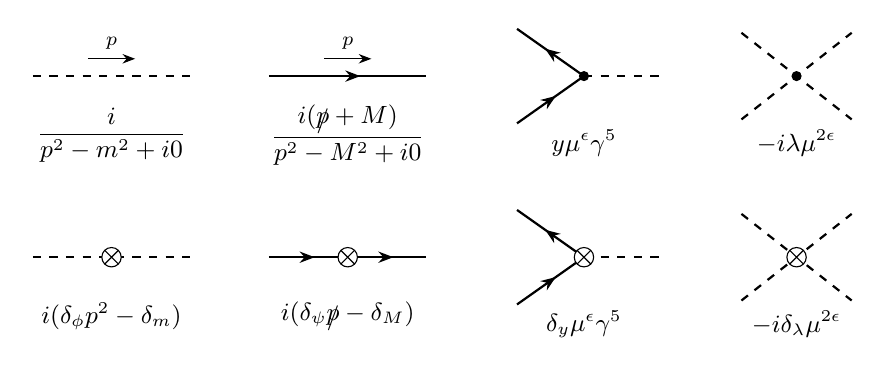
\begin{tikzpicture}
\begin{scope}[shift={(0,0)}]
  \draw[scalar] (0,0) -- (2,0);
  \draw[mom] (0.7,0.22) -- (1.3,0.22) node[midway,above,font=\scriptsize] {$p$};
  \node[lab] at (1,-0.75) {$\dfrac{i}{p^2-m^2+i0}$};
\end{scope}
\begin{scope}[shift={(3.0,0)}]
  \draw[fermion] (0,0) -- (2,0);
  \draw[mom] (0.7,0.22) -- (1.3,0.22) node[midway,above,font=\scriptsize] {$p$};
  \node[lab] at (1,-0.75) {$\dfrac{i(\slashed p+M)}{p^2-M^2+i0}$};
\end{scope}
\begin{scope}[shift={(7.0,0)}]
  \draw[fermion] (-0.85,-0.6) -- (0,0);
  \draw[fermion] (0,0) -- (-0.85,0.6);
  \draw[scalar] (0,0) -- (0.95,0);
  \node[vtx] at (0,0) {};
  \node[lab] at (0,-0.85) {$y\mu^{\epsilon}\gamma^5$};
\end{scope}
\begin{scope}[shift={(9.7,0)}]
  \draw[scalar] (-0.7,0.55) -- (0.7,-0.55) (-0.7,-0.55) -- (0.7,0.55);
  \node[vtx] at (0,0) {};
  \node[lab] at (0,-0.85) {$-i\lambda\mu^{2\epsilon}$};
\end{scope}
\begin{scope}[shift={(0,-2.3)}]
  \draw[scalar] (0,0) -- (2,0);
  \node[ctv] at (1,0) {};
  \node[lab] at (1,-0.75) {$i(\delta_\phi p^2-\delta_m)$};
\end{scope}
\begin{scope}[shift={(3.0,-2.3)}]
  \draw[fermion] (0,0) -- (1,0);
  \draw[fermion] (1,0) -- (2,0);
  \node[ctv] at (1,0) {};
  \node[lab] at (1,-0.75) {$i(\delta_\psi\slashed p-\delta_M)$};
\end{scope}
\begin{scope}[shift={(7.0,-2.3)}]
  \draw[fermion] (-0.85,-0.6) -- (0,0);
  \draw[fermion] (0,0) -- (-0.85,0.6);
  \draw[scalar] (0,0) -- (0.95,0);
  \node[ctv] at (0,0) {};
  \node[lab] at (0,-0.85) {$\delta_y\mu^{\epsilon}\gamma^5$};
\end{scope}
\begin{scope}[shift={(9.7,-2.3)}]
  \draw[scalar] (-0.7,0.55) -- (0.7,-0.55) (-0.7,-0.55) -- (0.7,0.55);
  \node[ctv] at (0,0) {};
  \node[lab] at (0,-0.85) {$-i\delta_\lambda\mu^{2\epsilon}$};
\end{scope}
\end{tikzpicture}
\caption{式~\eqref{eq:L} から導いた Feynman 則（\ref{app:rules}）。破線は $\phi$、矢印の付いた実線は $\psi$ で、矢印はフェルミオン数の流れの向きである。上の段は左から $\phi$ と $\psi$ の伝播関数、湯川の頂点、4点頂点。下の段はそれぞれの対抗項で、$\otimes$ は対抗項の挿入を表す。ループ運動量 $k$ ごとに $\int\dd^Dk/(2\pi)^D$ を掛け、対称性因子で割る。閉じたフェルミオンのループには $-1$ とトレースが付く。}
\label{fig:rules}
\end{figure}

\begin{figure}[tbp]
\centering
\begin{tikzpicture}
% row 1
\begin{scope}[shift={(0,0)}]
  \draw[scalar] (-1.5,0) -- (-0.55,0) (0.55,0) -- (1.5,0);
  \draw[fermion] (0.55,0) arc (0:180:0.55);
  \draw[fermion] (-0.55,0) arc (180:360:0.55);
  \node[vtx] at (-0.55,0) {}; \node[vtx] at (0.55,0) {};
  \node[lab] at (0,-0.95) {(a) $V_\phi$：$y^2$};
  \node[lab,font=\footnotesize] at (0,-1.4) {$1$（$-1$ とトレース）};
\end{scope}
\begin{scope}[shift={(4.4,-0.3)}]
  \draw[scalar] (-1.2,0) -- (1.2,0);
  \draw[scalar] (0,0.5) circle (0.5);
  \node[vtx] at (0,0) {};
  \node[lab] at (0,-0.65) {(b) $V_\phi$：$\lambda$};
  \node[lab,font=\footnotesize] at (0,-1.1) {$1/2$};
\end{scope}
\begin{scope}[shift={(8.8,-0.3)}]
  \draw[fermion] (-1.5,0) -- (-0.7,0);
  \draw[fermion] (-0.7,0) -- (0.7,0);
  \draw[fermion] (0.7,0) -- (1.5,0);
  \draw[scalar] (0.7,0) arc (0:180:0.7);
  \node[vtx] at (-0.7,0) {}; \node[vtx] at (0.7,0) {};
  \node[lab] at (0,-0.65) {(c) $V_\psi$：$y^2$};
  \node[lab,font=\footnotesize] at (0,-1.1) {$1$};
\end{scope}
% row 2
\begin{scope}[shift={(0,-3.4)}]
  \draw[fermion] (-1.5,0) -- (-0.75,0);
  \draw[fermion] (-0.75,0) -- (0,0);
  \draw[fermion] (0,0) -- (0.75,0);
  \draw[fermion] (0.75,0) -- (1.5,0);
  \draw[scalar] (0.75,0) arc (0:180:0.75);
  \draw[scalar] (0,0) -- (0,-0.8);
  \node[vtx] at (-0.75,0) {}; \node[vtx] at (0,0) {}; \node[vtx] at (0.75,0) {};
  \node[lab] at (0,-1.2) {(d) $V_y$：$y^3$};
  \node[lab,font=\footnotesize] at (0,-1.65) {$1$};
\end{scope}
\begin{scope}[shift={(4.4,-3.4)}]
  \draw[scalar] (-0.55,0) -- (-1.2,0.6) (-0.55,0) -- (-1.2,-0.6) (0.55,0) -- (1.2,0.6) (0.55,0) -- (1.2,-0.6);
  \draw[scalar] (0,0) circle (0.55);
  \node[vtx] at (-0.55,0) {}; \node[vtx] at (0.55,0) {};
  \node[lab] at (0,-1.2) {(e) $V_4$：$\lambda^2$（3通り）};
  \node[lab,font=\footnotesize] at (0,-1.65) {$1/2$};
\end{scope}
\begin{scope}[shift={(8.8,-3.4)}]
  \draw[fermion] (-0.55,-0.55) -- (0.55,-0.55);
  \draw[fermion] (0.55,-0.55) -- (0.55,0.55);
  \draw[fermion] (0.55,0.55) -- (-0.55,0.55);
  \draw[fermion] (-0.55,0.55) -- (-0.55,-0.55);
  \draw[scalar] (-0.55,0.55) -- (-1.0,1.0) (0.55,0.55) -- (1.0,1.0) (-0.55,-0.55) -- (-1.0,-1.0) (0.55,-0.55) -- (1.0,-1.0);
  \node[vtx] at (-0.55,0.55) {}; \node[vtx] at (0.55,0.55) {}; \node[vtx] at (-0.55,-0.55) {}; \node[vtx] at (0.55,-0.55) {};
  \node[lab] at (0,-1.2) {(f) $V_4$：$y^4$（6通り）};
  \node[lab,font=\footnotesize] at (0,-1.65) {$1$（$-1$ とトレース）};
\end{scope}
% row 3: vanishing
\begin{scope}[shift={(2.2,-6.9)}]
  \draw[scalar] (-1.1,0) -- (0,0);
  \draw[fermion] (0,0) arc (-90:270:0.5);
  \node[vtx] at (0,0) {};
  \node[lab] at (0,-0.55) {(g) 1点：$y$};
  \node[lab,font=\footnotesize] at (0,-1.0) {トレースで $0$};
\end{scope}
\begin{scope}[shift={(6.6,-6.9)}]
  \coordinate (A) at (-0.6,0); \coordinate (B) at (0.45,0.6); \coordinate (C) at (0.45,-0.6);
  \draw[fermion] (A) -- (B); \draw[fermion] (B) -- (C); \draw[fermion] (C) -- (A);
  \draw[scalar] (A) -- (-1.35,0) (B) -- (1.0,1.05) (C) -- (1.0,-1.05);
  \node[vtx] at (A) {}; \node[vtx] at (B) {}; \node[vtx] at (C) {};
  \node[lab] at (0,-1.4) {(h) 3点：$y^3$};
  \node[lab,font=\footnotesize] at (0,-1.85) {トレースで $0$};
\end{scope}
\end{tikzpicture}
\caption{1ループの1PI 図と、その対称性因子（\ref{app:rules}）。括弧は外線の付け方の数である。(a) と (f) は閉じたフェルミオンのループで、$-1$ とトレースが付く。(f) の6通りは、4本の外線をループに付ける巡回の順序（向きを区別して $3!=6$）である。(g) と (h) は $\gamma^5$ を奇数個含むトレースで0になり、パリティで禁じられた $\phi$ と $\phi^3$ の項が生じないことを表す（\ref{app:gamma5}）。}
\label{fig:oneloop}
\end{figure}

\paragraph{べき数え上げ。}外の $\phi$ 線 $E_\phi$ 本、外のフェルミオン線 $E_\psi$ 本の図の表面的な発散次数は、$d=4$ で
\begin{equation}
\omega=4-E_\phi-\frac32E_\psi
\label{eq:omega}
\end{equation}
である（\ref{app:counting}）。湯川の頂点と4点頂点はどちらも無次元の結合なので、$\omega$ は頂点の数によらない。$\omega\ge0$ となるのは、$(E_\phi,E_\psi)=(1,0),(2,0),(3,0),(4,0),(0,2),(1,2)$ の6種類である。このうち $\phi$ の1点関数と3点関数はパリティで0になる。残りの4種類が図~\ref{fig:oneloop} の $V_\phi$（$\omega=2$）、$V_4$（$\omega=0$）、$V_\psi$（$\omega=1$）、$V_y$（$\omega=0$）で、式~\eqref{eq:L} の対抗項がちょうどそれらに対応する。$\phi\phi\psi\bar\psi$ の4点関数（$\omega=-1$）と、フェルミオン4本の関数（$\omega=-2$）は有限である。

\paragraph{パリティと消える図。}1ループで $\phi$ の1点関数を作る図は、フェルミオンのループ (g) だけである。そのトレース $\mathrm{tr}[\gamma^5(\slashed k+M)]$ は0である。$\phi$ の3点関数を作る図はフェルミオンの三角形 (h) で、そのトレースは $\gamma^5$ を3つ含み、$\gamma^5$ を1つにまとめると、残りの $\gamma$ 行列は3個以下になる。$\gamma^5$ と3個以下の $\gamma$ 行列のトレースは0なので、(h) も0である（\ref{app:gamma5}）。これらが0になるのは、パリティが $\phi$ と $\phi^3$ の項を禁じることの1ループでの現れである。したがって、本模型には線形項 $Y\phi$ も3点結合も要らない。

\paragraph{1ループの1PI 関数。}伝播関数の分母を $D_a(k)\equiv k^2-m_a^2+i0$（$m_a=m$ または $M$）と書き、1点と2点のスカラー積分を
\begin{equation}
I_1^a\equiv\int\frac{\dd^Dk}{(2\pi)^D}\frac{1}{D_a(k)},\qquad
I_2^{ab}(p^2)\equiv\int\frac{\dd^Dk}{(2\pi)^D}\frac{1}{D_a(k)\,D_b(k+p)}
\label{eq:IN}
\end{equation}
と定義する。図~\ref{fig:oneloop} の図を Feynman 則で書き、トレースと $\gamma^5$ を整理して対抗項を加えると
\begin{equation}
\begin{aligned}
V_\phi(p^2)&=2y^2\mu^{2\epsilon}\bigl[p^2I_2^{MM}(p^2)-2I_1^M\bigr]+\frac{\lambda\mu^{2\epsilon}}{2}\,I_1^m+i\bigl(\delta_\phi p^2-\delta_m\bigr),\\
V_\psi(p)&=y^2\mu^{2\epsilon}\int\frac{\dd^Dk}{(2\pi)^D}\frac{\slashed k-M}{D_M(k)\,D_m(k-p)}+i\bigl(\delta_\psi\slashed p-\delta_M\bigr),\\
V_y&=-iy^3\mu^{3\epsilon}\int\frac{\dd^Dk}{(2\pi)^D}\frac{\bigl(M^2-k^2-M\slashed q-\slashed q\slashed k\bigr)\gamma^5}{D_M(k+q)\,D_M(k)\,D_m(k-p)}+\delta_y\mu^\epsilon\gamma^5,\\
V_4&=\frac{\lambda^2\mu^{4\epsilon}}{2}\sum_{x=s,t,u}I_2^{mm}(x)-y^4\mu^{4\epsilon}\sum_{(6)}\int\frac{\dd^Dk}{(2\pi)^D}\frac{T}{D_M(k_1)D_M(k_2)D_M(k_3)D_M(k_4)}-i\,\delta_\lambda\mu^{2\epsilon}
\end{aligned}
\label{eq:V}
\end{equation}
となる（\ref{app:ren}）。$V_\psi$ の $p$ は入ってくるフェルミオンの運動量である。$V_y$ では、入ってくるフェルミオンの運動量を $p$、入ってくる $\phi$ の運動量を $q$、出ていくフェルミオンの運動量を $p'=p+q$ とした。$V_4$ の $k_1,\dots,k_4$ は箱の4本の伝播関数の運動量で、トレースは $T=\mathrm{tr}[(M-\slashed k_1)(M+\slashed k_2)(M-\slashed k_3)(M+\slashed k_4)]$ である。$\gamma^5(\slashed a+M)\gamma^5=-\slashed a+M$ を使って $\gamma^5$ を消した。$V_\phi$ の第1項の符号は、閉じたフェルミオンのループの $-1$ から来る。

\paragraph{$\MSbar$ の対抗項。}$d=4$ で発散するのは、$I_1$、$I_2$、ベクトルの2点積分、および $V_y$ と $V_4$ の中で分子の運動量の2乗が分母の運動量の2乗を打ち消す項である。極を取り出すと（\ref{app:ren}）、式~\eqref{eq:V} の極を消す対抗項は
\begin{equation}
\begin{gathered}
\delta_\phi=-\frac{2y^2}{(4\pi)^2}\Delta_{\mathrm{UV}},\qquad
\delta_m=\frac{1}{(4\pi)^2}\Bigl(\frac{\lambda m^2}{2}-4y^2M^2\Bigr)\Delta_{\mathrm{UV}},\qquad
\delta_\psi=-\frac{y^2}{2(4\pi)^2}\Delta_{\mathrm{UV}},\\
\delta_M=-\frac{y^2M}{(4\pi)^2}\Delta_{\mathrm{UV}},\qquad
\delta_y=\frac{y^3}{(4\pi)^2}\Delta_{\mathrm{UV}},\qquad
\delta_\lambda=\frac{1}{(4\pi)^2}\Bigl(\frac{3\lambda^2}{2}-24y^4\Bigr)\Delta_{\mathrm{UV}}
\end{gathered}
\label{eq:ct}
\end{equation}
である。$\phi^3+\phi^4$ 理論と違って、$\phi$ の場の対抗項 $\delta_\phi$ が0でなくなる。これはフェルミオンのループ (a) の極が $p^2$ に比例する部分を持つからで、閉じたループの $-1$ のために $\delta_\phi<0$ である。$\delta_\lambda$ の $-24y^4$ はフェルミオンの箱 (f) の6つの図から来て、やはり $-1$ のために負である。$\delta_M$ の符号は、スカラーの湯川結合 $y\phi\bar\psi\psi$ の場合と逆になる。$\gamma^5$ がフェルミオンの伝播関数の質量の項の符号を反転させるからである。

\paragraph{繰り込まれた1PI 関数。}式~\eqref{eq:ct} を式~\eqref{eq:V} に入れて $\epsilon\to0$ とすると
\begin{equation}
\begin{aligned}
V_\phi(p^2)&=\frac{i}{(4\pi)^2}\Bigl[2y^2\bigl(p^2B_0^{MM}(p^2)-2A_0(M^2)\bigr)+\frac{\lambda}{2}A_0(m^2)\Bigr],\\
V_\psi(p)&=-\frac{iy^2}{(4\pi)^2}\Bigl[\slashed p\,B_1^{Mm}(p^2)+M\,B_0^{Mm}(p^2)\Bigr],\\
V_y&=-\frac{y^3}{(4\pi)^2}\Bigl[B_0^{Mm}(p'^2)+M\slashed q\,C_0+q^2C_1-\slashed q\slashed p\,C_2\Bigr]\gamma^5,\\
V_4&=\frac{i}{(4\pi)^2}\Bigl[\frac{\lambda^2}{2}\sum_{x=s,t,u}B_0^{mm}(x)-2y^4\sum_{(x,x')}\mathcal F(x,x')\Bigr]
\end{aligned}
\label{eq:VR}
\end{equation}
となる（\ref{app:ren}）。$A_0$、$B_0$、$B_1$、$C_i$ は LoopTools の規約の $\MSbar$ の有限部分で、$B_1$ は $\int\dd^Dk\,k^\mu/(D_a(k)D_b(k+p))$ の $p^\mu$ の係数、$C_i\equiv C_i(q^2,p'^2,p^2;M^2,M^2,m^2)$ である。$V_4$ は外線の $\phi$ がすべて質量殻上（$p_i^2=m^2$）のときの値で、和は $(x,x')=(s,t),(t,u),(u,s)$ についてとる。フェルミオンの箱の図の和は
\begin{equation}
\mathcal F(x,x')=(2m^4-xx')\,D_0^{M}(x,x')+2\bigl[B_0^{MM}(x)+B_0^{MM}(x')\bigr]+2(x-2m^2)\,C_0^{M}(x)+2(x'-2m^2)\,C_0^{M}(x')
\label{eq:box}
\end{equation}
となる。ここで $C_0^M(x)\equiv C_0(m^2,m^2,x;M^2,M^2,M^2)$、$D_0^M(x,x')$ は外線の質量の2乗がすべて $m^2$ で、二つのチャンネルの不変量が $x$、$x'$ の箱の積分（内線の質量はすべて $M$）である。この短い形は、トレース $T$ の中の内積 $k_i\cdot k_j$ を分母 $D_M(k_i)$、$D_M(k_j)$ と外線の不変量で書き直すと、$T$ が分母の2次式になることから得られる（\ref{app:ren}）。その際、$T$ の定数項からフェルミオンの質量 $M$ は消える。自己エネルギーは
\begin{equation*}
\Sigma_\phi=-\frac{1}{(4\pi)^2}\Bigl[2y^2\bigl(p^2B_0^{MM}(p^2)-2A_0(M^2)\bigr)+\frac{\lambda}{2}A_0(m^2)\Bigr],\qquad
\Sigma_\psi=\frac{y^2}{(4\pi)^2}\Bigl[\slashed p\,B_1^{Mm}(p^2)+M\,B_0^{Mm}(p^2)\Bigr]
\end{equation*}
である。

\paragraph{繰り込み群。}裸の量が $\mu$ によらないことから
\begin{equation}
\begin{gathered}
\beta_y=\frac{5y^3}{(4\pi)^2},\qquad
\beta_\lambda=\frac{3\lambda^2+8\lambda y^2-48y^4}{(4\pi)^2},\qquad
\gamma_m=\frac{\lambda m^2+4y^2m^2-8y^2M^2}{(4\pi)^2},\\
\gamma_M=-\frac{y^2M}{(4\pi)^2},\qquad
\gamma_\phi=\frac{2y^2}{(4\pi)^2},\qquad
\gamma_\psi=\frac{y^2}{2(4\pi)^2}
\end{gathered}
\label{eq:rge}
\end{equation}
を得る（\ref{app:rg}）。$\beta_y$ の係数5は、頂点 (d) の $2$ と、場の繰り込みからの $2\gamma_\psi+\gamma_\phi$ の $3$ の和である。$\beta_\lambda$ の三つの項は、$\phi$ の泡 (e)（$3\lambda^2$）、外線4本の場の繰り込み（$4\gamma_\phi\lambda=8\lambda y^2$）、フェルミオンの箱 (f)（$-48y^4$）から来る。$\gamma_M$ が負であることも、スカラーの湯川結合（$+3y^2M/(4\pi)^2$）と違う点である。$M=0$ では、カイラル回転 $\psi\to e^{i\pi\gamma^5/4}\psi$ で擬スカラーの湯川結合はスカラーの湯川結合に移るので、質量によらない $\beta_y$、$\beta_\lambda$、$\gamma_\phi$、$\gamma_\psi$ は両者で同じである（\ref{app:gamma5}）。

1ループでは、比 $r\equiv\lambda/y^2$ の流れが解析的に解ける（\ref{app:rg}）。$\dd r/\dd\ln\mu=y^2(3r^2-2r-48)/(4\pi)^2$ で、その零点は $r_\pm=(1\pm\sqrt{145})/3$（$r_+=4.3472$、$r_-=-3.6805$）である。$\mu=\mu_0$ での値を $r_0$、$y_0$ とすると
\begin{equation}
\frac{r-r_+}{r-r_-}=\frac{r_0-r_+}{r_0-r_-}\Bigl(\frac{y^2}{y_0^2}\Bigr)^{\sqrt{145}/5},\qquad
\frac{y^2}{y_0^2}=\frac{1}{1-10y_0^2\ln(\mu/\mu_0)/(4\pi)^2}
\label{eq:rflow}
\end{equation}
となる。$y^2$ は $\mu$ とともに増え、$\ln(\mu_{\mathrm L}/\mu_0)=(4\pi)^2/(10y_0^2)$ で Landau 極に達する。$r_0<r_+$ なら $r$ は減り続けて0を横切り、Landau 極で $r_-$ に近づく。すなわち、$\lambda$ は $y$ の Landau 極より先に負になる。$r_0>r_+$ なら $r$ は増え続け、$\lambda$ のほうが先に発散する。$r=r_+$ は低エネルギーで引きつける固定点である。基準点 $y_0=\lambda_0=1$、$\mu_0=m$ では、$\lambda$ は $\mu=19.49\,m$ で0になり、$y$ の Landau 極は $\mu_{\mathrm L}=7.2\times10^6\,m$ にある。$\lambda$ が負になることは、次の有効ポテンシャルが大きな場で下に有界でなくなることを意味し、手順 (9)、(10) で調べる真空の不安定性の出発点になる。

\paragraph{有効ポテンシャル。}$\MSbar$ の1ループの有効ポテンシャルは
\begin{equation}
\begin{gathered}
V_{\mathrm{eff}}(\phi)=\Lambda+\frac12m^2\phi^2+\frac{\lambda}{24}\phi^4
+\frac{1}{64\pi^2}\Bigl[m_\phi^4\Bigl(\ln\frac{m_\phi^2}{\mu^2}-\frac32\Bigr)-4M_\psi^4\Bigl(\ln\frac{M_\psi^2}{\mu^2}-\frac32\Bigr)\Bigr],\\
m_\phi^2(\phi)=m^2+\frac{\lambda}{2}\phi^2,\qquad M_\psi^2(\phi)=M^2+y^2\phi^2
\end{gathered}
\label{eq:cw}
\end{equation}
である（Coleman と Weinberg~\cite{cw}、導出は\ref{app:rg}）。$\Lambda$ は真空のエネルギーである。フェルミオンの項の係数 $-4$ は、Dirac フェルミオンの自由度4と、Grassmann 数の積分の符号から来る。擬スカラーの湯川結合では、場に依存する質量は $M_\psi^2=M^2+y^2\phi^2$ で、$\phi$ の1次の項を持たない（スカラーの湯川結合では $(M+y\phi)^2$）。$V_{\mathrm{eff}}$ の $\mu$ 依存が、係数の走りと場の異常次元で打ち消される条件から、式~\eqref{eq:rge} の $\beta_\lambda$ と $\gamma_m$ が再び得られ、真空のエネルギーの走り $\dd\Lambda/\dd\ln\mu=(m^4-4M^4)/(2(4\pi)^2)$ も決まる。木のポテンシャルの極小は $\phi=0$ だけだが、大きな $\phi$ ではフェルミオンの項 $-4y^4\phi^4\ln(y^2\phi^2/\mu^2)/(64\pi^2)$ が効き、$\mu\sim\phi$ での $\lambda$ が負なら $V_{\mathrm{eff}}$ は下に有界でなくなる。

\paragraph{木の散乱振幅。}三つの過程を考える（図~\ref{fig:tree}、\ref{app:tree}）。$\phi(p_1)\phi(p_2)\to\phi(k_1)\phi(k_2)$ は、3点結合がないので接触項だけである。$\psi(p_1)\bar\psi(p_2)\to\phi(k_1)\phi(k_2)$ は $t$ と $u$ チャンネルのフェルミオンの交換で、$s$ チャンネルの図はない。$\psi(p_1)\bar\psi(p_2)\to\psi(p_3)\bar\psi(p_4)$ は $s$ と $t$ チャンネルの $\phi$ の交換で、二つの図の相対符号は $-1$ である。振幅とスピン和は
\begin{equation}
\begin{aligned}
\mathcal M_A^{(0)}&=-\lambda,\\
\mathcal M_B^{(0)}&=y^2\,\bar v(p_2)\Bigl[\frac{\slashed k_1}{t-M^2}+\frac{\slashed k_2}{u-M^2}\Bigr]u(p_1),\qquad
\sum|\mathcal M_B^{(0)}|^2=\frac{2y^4\bigl[(t-M^2)(u-M^2)-m^4\bigr](t-u)^2}{(t-M^2)^2(u-M^2)^2},\\
\sum|\mathcal M_C^{(0)}|^2&=4y^4\Bigl[\frac{s^2}{(s-m^2)^2}+\frac{t^2}{(t-m^2)^2}+\frac{st}{(s-m^2)(t-m^2)}\Bigr]
\end{aligned}
\label{eq:Mtree}
\end{equation}
である（\ref{app:tree}）。$\mathcal{M}_B$ では、質量殻上の $\bar v(p_2)$ と $u(p_1)$ に挟まれて、交換されるフェルミオンの運動量 $\slashed p_1$ と質量 $M$ の項が消えた。重心系で $\psi$ と $\phi$ の運動量の大きさを $p$、$k$、散乱角を $\theta$ とすると、$t-u=4pk\cos\theta$、$(t-M^2)(u-M^2)-m^4=k^2(s-4p^2\cos^2\theta)$ なので
\begin{equation*}
\sum|\mathcal M_B^{(0)}|^2=\frac{32y^4p^2k^4\cos^2\theta\,(s-4p^2\cos^2\theta)}{(t-M^2)^2(u-M^2)^2}
\end{equation*}
となる（\ref{app:tree}）。$p^2$ に比例するので、$\psi\bar\psi$ の閾値（$p\to0$）の近くでは、$\psi\bar\psi\to\phi\phi$ は p 波から始まり、$\sigma v\propto v^2$ である。これは、S 波の $\psi\bar\psi$（${}^1S_0$ と ${}^3S_1$）のパリティがどちらも負で、同種の擬スカラー2つの状態（軌道角運動量が偶数なのでパリティが正）に移れないことの現れである。ただし、$\psi\bar\psi$ の閾値で $\phi\phi$ を作れるのは $m<M$ のときだけである。基準点のように $m>M$ では、断面積は $\phi\phi$ の閾値（$k\to0$）から始まり、$\sum|\mathcal M_B|^2\propto k^4$、すなわち $\sigma_B\propto k^5$ と、終状態が D 波であるようにふるまう。$\sum|\mathcal M_C|^2$ には $M$ が陽に現れない。$\bar\psi\gamma^5\psi$ の型の双一次形式の2乗のスピン和が、$2s$、$-2t$、$-2st$ のように質量によらない形になるからで、$M$ は運動学（$s+t+u=4M^2$）を通してだけ入る。

\begin{figure}[tbp]
\centering
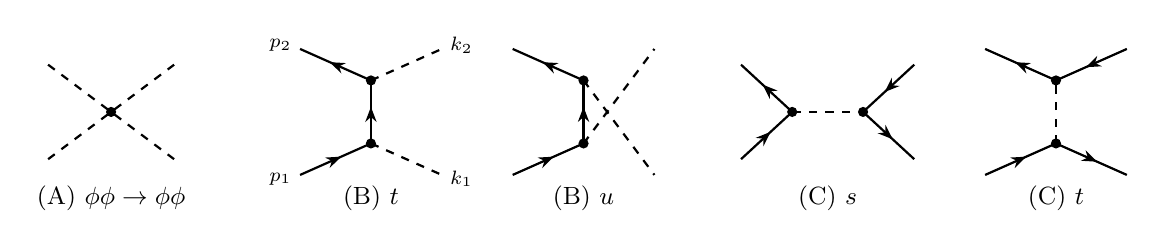
\begin{tikzpicture}
\begin{scope}[shift={(0,0)}]
  \draw[scalar] (-0.8,0.6) -- (0.8,-0.6) (-0.8,-0.6) -- (0.8,0.6);
  \node[vtx] at (0,0) {};
  \node[lab] at (0,-1.1) {(A) $\phi\phi\to\phi\phi$};
\end{scope}
\begin{scope}[shift={(3.3,0)}]
  \draw[fermion] (-0.9,-0.8) -- (0,-0.4);
  \draw[fermion] (0,-0.4) -- (0,0.4);
  \draw[fermion] (0,0.4) -- (-0.9,0.8);
  \draw[scalar] (0,-0.4) -- (0.9,-0.8) (0,0.4) -- (0.9,0.8);
  \node[vtx] at (0,-0.4) {}; \node[vtx] at (0,0.4) {};
  \node[font=\scriptsize] at (-1.15,-0.85) {$p_1$}; \node[font=\scriptsize] at (-1.15,0.85) {$p_2$};
  \node[font=\scriptsize] at (1.15,-0.85) {$k_1$}; \node[font=\scriptsize] at (1.15,0.85) {$k_2$};
  \node[lab] at (0,-1.1) {(B) $t$};
\end{scope}
\begin{scope}[shift={(6.0,0)}]
  \draw[fermion] (-0.9,-0.8) -- (0,-0.4);
  \draw[fermion] (0,-0.4) -- (0,0.4);
  \draw[fermion] (0,0.4) -- (-0.9,0.8);
  \draw[scalar] (0,-0.4) -- (0.9,0.8) (0,0.4) -- (0.9,-0.8);
  \node[vtx] at (0,-0.4) {}; \node[vtx] at (0,0.4) {};
  \node[lab] at (0,-1.1) {(B) $u$};
\end{scope}
\begin{scope}[shift={(9.1,0)}]
  \draw[fermion] (-1.1,-0.6) -- (-0.45,0);
  \draw[fermion] (-0.45,0) -- (-1.1,0.6);
  \draw[fermion] (1.1,0.6) -- (0.45,0);
  \draw[fermion] (0.45,0) -- (1.1,-0.6);
  \draw[scalar] (-0.45,0) -- (0.45,0);
  \node[vtx] at (-0.45,0) {}; \node[vtx] at (0.45,0) {};
  \node[lab] at (0,-1.1) {(C) $s$};
\end{scope}
\begin{scope}[shift={(12.0,0)}]
  \draw[fermion] (-0.9,-0.8) -- (0,-0.4);
  \draw[fermion] (0,-0.4) -- (0.9,-0.8);
  \draw[fermion] (0.9,0.8) -- (0,0.4);
  \draw[fermion] (0,0.4) -- (-0.9,0.8);
  \draw[scalar] (0,-0.4) -- (0,0.4);
  \node[vtx] at (0,-0.4) {}; \node[vtx] at (0,0.4) {};
  \node[lab] at (0,-1.1) {(C) $t$};
\end{scope}
\end{tikzpicture}
\caption{木の図。(A) $\phi\phi\to\phi\phi$ の接触項。(B) $\psi(p_1)\bar\psi(p_2)\to\phi(k_1)\phi(k_2)$ の $t$、$u$ チャンネルのフェルミオンの交換。(C) $\psi\bar\psi\to\psi\bar\psi$ の $s$、$t$ チャンネルの $\phi$ の交換（相対符号 $-1$）。時間は左から右に流れる。}
\label{fig:tree}
\end{figure}

全断面積は、重心系の始状態と終状態の運動量の大きさを $p$、$k$ として
\begin{equation}
\sigma_A=\frac{\lambda^2}{32\pi s},\qquad
\sigma_B=\frac12\,\frac{k}{64\pi^2sp}\int\!\dd\Omega\,\frac14\sum|\mathcal M_B^{(0)}|^2,\qquad
\sigma_C=\frac{1}{64\pi^2s}\int\!\dd\Omega\,\frac14\sum|\mathcal M_C^{(0)}|^2
\label{eq:sigma}
\end{equation}
である（\ref{app:tree}）。$\frac14$ は始状態のスピンの平均、$\sigma_A$ と $\sigma_B$ の $\frac12$ は終状態の同種の $\phi$ の因子である。$\psi\bar\psi\to\psi\bar\psi$ の終状態の $\psi$ と $\bar\psi$ は区別できるので、$\frac12$ は付かない。

\paragraph{1ループの $\phi\phi\to\phi\phi$ と S 行列要素。}3点結合がないので、$\phi\phi\to\phi\phi$ の1ループの振幅（外線の補正を除く）は1PI の4点関数だけで、$i\mathcal M_A^{(1)}=V_4$ である。式~\eqref{eq:VR} から
\begin{equation}
(4\pi)^2\,\mathcal M_A^{(1)}=\frac{\lambda^2}{2}\sum_{x=s,t,u}B_0^{mm}(x)-2y^4\sum_{(x,x')}\mathcal F(x,x')
\label{eq:M1}
\end{equation}
を得る。虚部は $s$ チャンネルのユニタリー性
\begin{equation}
\mathrm{Im}\,\mathcal M_A^{(1)}(s,t)=\frac{\lambda^2p}{16\pi\sqrt s}
+\frac12\,\frac{p_\psi}{16\pi^2\sqrt s}\int\!\dd\Omega_q\sum_{\mathrm{spins}}\mathcal M(\phi_1\phi_2\to\psi\bar\psi)\,\mathcal M^*(\phi_3\phi_4\to\psi\bar\psi)
\label{eq:unit}
\end{equation}
を満たす（\ref{app:scat}）。第1項は $\phi\phi$ の中間状態（同種粒子の $\frac12$ を含む）、第2項は $\psi\bar\psi$ の中間状態で、$p_\psi=\sqrt{s/4-M^2}$、$\phi_3\phi_4$ は終状態の $\phi(k_1)\phi(k_2)$ である。$m<2M$ でも $s\ge4m^2>4M^2$ なので、物理的な領域では $\psi\bar\psi$ の中間状態がいつも開いている。前方 $t=0$ では、これは光学定理 $\mathrm{Im}\,\mathcal M_A^{(1)}(s,0)=2p\sqrt s\,[\sigma_A+\sigma(\phi\phi\to\psi\bar\psi)]$ になる。$\sum|\mathcal M(\phi\phi\to\psi\bar\psi)|^2$ は式~\eqref{eq:Mtree} の $\sum|\mathcal M_B^{(0)}|^2$ と同じ関数である。

$\MSbar$ の質量 $m$ は伝播関数の極ではなく、外線の留数も1ではない。$\phi$ の極質量と留数は
\begin{equation}
m_{\mathrm p}^2=m^2-\frac{1}{(4\pi)^2}\Bigl[2y^2\bigl(m^2B_0^{MM}(m^2)-2A_0(M^2)\bigr)+\frac\lambda2A_0(m^2)\Bigr],\qquad
R_\phi=1-\frac{2y^2}{(4\pi)^2}\Bigl[B_0^{MM}(m^2)+m^2B_0^{MM\prime}(m^2)\Bigr]
\label{eq:mpole}
\end{equation}
である（\ref{app:scat}）。$\phi^3+\phi^4$ 理論と違い、フェルミオンのループのために $R_\phi$ は $y^2$ の次数で1からずれ、$\mu$ にも依存する（$\mu\,\dd R_\phi/\dd\mu=-2\gamma_\phi$）。木の振幅 $-\lambda$ は質量によらないので、S 行列要素 $R_\phi^2(\mathcal M_A^{(0)}+\mathcal M_A^{(1)})$ は
\begin{equation}
\mathcal M_{A,\mathrm{phys}}=-\lambda+\frac{4\lambda y^2}{(4\pi)^2}\Bigl[B_0^{MM}(m_{\mathrm p}^2)+m_{\mathrm p}^2B_0^{MM\prime}(m_{\mathrm p}^2)\Bigr]+\mathcal M_A^{(1)}\big|_{m\to m_{\mathrm p}}
\label{eq:Mphys}
\end{equation}
となる。結合を固定して $\mu$ を変えると $\mu\,\partial\mathcal M_{A,\mathrm{phys}}/\partial\mu=(3\lambda^2+8\lambda y^2-48y^4)/(4\pi)^2=\beta_\lambda$ で、これは木の振幅の $-\lambda(\mu)$ の走りとちょうど打ち消し合う（\ref{app:scat}）。$3\lambda^2$ は $\phi$ の泡、$-48y^4$ はフェルミオンの箱、$8\lambda y^2$ は外線の留数から来るので、$\phi\phi\to\phi\phi$ の S 行列要素の $\mu$ 依存だけで $\beta_\lambda$ の三つの項がすべて読み取れる。

フェルミオンの極質量と留数は、$\Sigma_\psi=\slashed p\,\Sigma_V(p^2)+M\Sigma_S(p^2)$（$\Sigma_V=y^2B_1^{Mm}/(4\pi)^2$、$\Sigma_S=y^2B_0^{Mm}/(4\pi)^2$）から
\begin{equation}
M_{\mathrm p}=M\Bigl[1+\frac{y^2}{(4\pi)^2}\bigl(B_0^{Mm}+B_1^{Mm}\bigr)\Bigr],\qquad
R_\psi=1+\frac{y^2}{(4\pi)^2}\Bigl[B_1^{Mm}+2M^2\bigl(B_0^{Mm\prime}+B_1^{Mm\prime}\bigr)\Bigr]
\label{eq:Mpole}
\end{equation}
である（\ref{app:scat}）。$B$ はすべて $p^2=M^2$ での値である。$M_{\mathrm p}$ は $\mu$ によらず（$\mu\,\partial(B_0+B_1)/\partial\mu=1$ と $\gamma_M$ が打ち消す）、外線のフェルミオン1本ごとに S 行列要素に $R_\psi^{1/2}$ が掛かる。これらは $\psi\bar\psi\to\phi\phi$ の1ループの S 行列要素（手順 (5)）で使う。

\paragraph{1ループの $\psi\bar\psi\to\phi\phi$。}外線にフェルミオンを持つ過程の1ループの振幅も、手で閉じた形に書ける。外線の補正を除いた1ループの図は、内線のフェルミオンの自己エネルギー（$t$、$u$ チャンネルに1つずつ）、頂点の補正（4つ）、箱（2つ）、$\phi$ の2本の内線が4点頂点で終わる三角形（$\lambda$ の三角形、1つ）、$s$ チャンネルの $\phi$ にフェルミオンの三角形が付いた図（2つ）の11個である。最後の2つはトレースが $\gamma^5$ と3個以下の $\gamma$ 行列しか含まないので0になる。Dirac 方程式と $k_2=p_1+p_2-k_1$ を使うと、どの図も二つのスピノルの構造 $\bar v(p_2)u(p_1)$ と $\bar v(p_2)\slashed k_1u(p_1)$ だけで書ける（$\bar v(p_2)(\slashed p_1+\slashed p_2)u(p_1)=0$ なので $\bar v\slashed k_2u=-\bar v\slashed k_1u$）。木の振幅は $b^{(0)}\bar v\slashed k_1u$、$b^{(0)}=y^2[1/(t-M^2)-1/(u-M^2)]$ である。$\MSbar$ で繰り込んだ1ループの振幅は
\begin{equation}
\begin{aligned}
(4\pi)^2\mathcal M_B^{(1)}={}&a\,\bar v(p_2)u(p_1)+b\,\bar v(p_2)\slashed k_1u(p_1),\\
a={}&\lambda y^2M\,C^\lambda_1+y^4M\sum_{x=t,u}\Bigl\{\frac{B_0(x)+B_1(x)}{x-M^2}-\bigl[C^{(1)}_0+C^{(1)}_2+C^{(2)}_0+C^{(2)}_2\bigr](x)\\
&\qquad-(x-M^2)\bigl[D_1+D_2+D_3\bigr](x)+C^s_1+C^s_2\Bigr\},\\
b={}&y^4\sum_{x=t,u}\sigma_x\Bigl\{\frac{(x+M^2)B_1(x)+2M^2B_0(x)}{(x-M^2)^2}-\frac{B_0(x)+m^2C^{(1)}_1(x)+2M^2\bigl[C^{(1)}_0+C^{(1)}_2\bigr](x)}{x-M^2}\\
&\qquad-\frac{B_0(M^2)+m^2C^{(2)}_1(x)+2M^2C^{(2)}_0(x)+(x+M^2)C^{(2)}_2(x)}{x-M^2}\\
&\qquad+m^2D_0(x)+C_0^M(s)+(x-M^2)D_2(x)\Bigr\}
\end{aligned}
\label{eq:M1B}
\end{equation}
である（\ref{app:scatB}）。$\sigma_t=1$、$\sigma_u=-1$ で、積分は LoopTools の規約の $\MSbar$ の有限部分である。$B_n(x)\equiv B_n(x;M^2,m^2)$、頂点の積分は $C^{(1)}_n(x)\equiv C_n(m^2,x,M^2;M^2,M^2,m^2)$（$\psi(p_1)$ の側）と $C^{(2)}_n(x)\equiv C_n(m^2,M^2,x;M^2,M^2,m^2)$（$\bar\psi(p_2)$ の側）、箱は $D_n(x)\equiv D_n(M^2,m^2,m^2,M^2,x,s;m^2,M^2,M^2,M^2)$、箱から $\phi$ 以外の内線を1本除いた三角形は $C^s_n\equiv C_n(M^2,s,M^2;m^2,M^2,M^2)$ と $C_0^M(s)$、$\lambda$ の三角形は $C^\lambda_1\equiv C_1(M^2,M^2,s;m^2,M^2,m^2)$ である。$a$ の各項は順に、$\lambda$ の三角形、自己エネルギー、二つの頂点の補正、箱から来る。$\lambda$ の三角形は $\bar vu$ の構造だけを持つ。箱は、分子の $\slashed\ell$ を Dirac 方程式と伝播関数の分母で消すと、テンソル積分を経ずに $D_0$、$D_{1,2,3}$、三角形の積分で書ける（\ref{app:scatB}）。虚部は $s$ チャンネルのユニタリー性
\begin{equation}
\begin{aligned}
\frac{\mathrm{Im}\,a\,\bar vu+\mathrm{Im}\,b\,\bar v\slashed k_1u}{(4\pi)^2}
={}&\frac12\frac{p}{16\pi^2\sqrt s}\int\!\dd\Omega_q\sum_{\mathrm{spins}}\mathcal M_C(\psi\bar\psi\to\psi_q\bar\psi_q)\,\mathcal M^*(\phi\phi\to\psi_q\bar\psi_q)\\
&+\frac14\frac{k}{16\pi^2\sqrt s}\int\!\dd\Omega_q\,\mathcal M_B^{(0)}(\psi\bar\psi\to\phi_q\phi_q)\,(-\lambda)
\end{aligned}
\label{eq:unitB}
\end{equation}
を満たす（\ref{app:scatB}）。右辺の第1項は $\psi\bar\psi$ の中間状態（$|\boldsymbol q|=p$）、第2項は $\phi\phi$ の中間状態（$|\boldsymbol q|=k$、同種粒子の $\frac12$）で、外線のスピンを固定した等式である。

S 行列要素は、外線の運動量とスピノルを極質量で定め、LSZ の簡約公式で外線ごとに留数の平方根 $R_\psi^{1/2}$、$R_\phi^{1/2}$ を掛けて得る。$\phi\phi\to\phi\phi$ では木の振幅が質量によらないので式~\eqref{eq:Mphys} になったが、$\psi\bar\psi\to\phi\phi$ では木の振幅の中のフェルミオンの質量が二か所で効く。交換されるフェルミオンの伝播関数の分母と、Dirac 方程式で消した項 $(M-\slashed p_1)u$ である。後者は外線のスピノルが極質量 $M_{\mathrm p}$ を持つので $(M-M_{\mathrm p})u$ として残り、新しい構造 $\bar vu$ を作る。式~\eqref{eq:Mpole} を使ってまとめると（\ref{app:scatB}）
\begin{equation}
\begin{aligned}
(4\pi)^2\mathcal M_{B,\mathrm{phys}}={}&(4\pi)^2b^{(0)}\big|_{M\to M_{\mathrm p}}\,\bar v\slashed k_1u+a_{\mathrm{phys}}\,\bar vu+b_{\mathrm{phys}}\,\bar v\slashed k_1u,\\
a_{\mathrm{phys}}={}&a-y^4M\bigl[B_0+B_1\bigr](M^2)\Bigl[\frac{1}{t-M^2}+\frac{1}{u-M^2}\Bigr],\\
b_{\mathrm{phys}}={}&b+y^2\Bigl\{\bigl[B_1+2M^2(B_0'+B_1')\bigr](M^2)-2\bigl[B_0^{MM}+m^2B_0^{MM\prime}\bigr](m^2)\Bigr\}b^{(0)}\\
&-2M^2y^4\bigl[B_0+B_1\bigr](M^2)\Bigl[\frac{1}{(t-M^2)^2}-\frac{1}{(u-M^2)^2}\Bigr]
\end{aligned}
\label{eq:MphysB}
\end{equation}
となる。$B_n(M^2)\equiv B_n(M^2;M^2,m^2)$ で、1ループの項の中の質量は極質量としてよい。$a_{\mathrm{phys}}$ の補正はフェルミオンの質量のずれ（Dirac 方程式の項）、$b_{\mathrm{phys}}$ の第2項は二つの留数、第3項は伝播関数の分母の質量のずれから来る。$\phi$ の質量は木の伝播関数に現れないので、運動学を通してしか入らない。結合を固定して $\mu$ を変えると $\partial a_{\mathrm{phys}}/\partial\ln\mu=0$、$\partial b_{\mathrm{phys}}/\partial\ln\mu=-10y^2b^{(0)}$ で、木の振幅 $b^{(0)}\propto y^2$ の $y(\mu)$ の走り（$\dd y^2/\dd\ln\mu=10y^4/(4\pi)^2$）とちょうど打ち消し合う。

\paragraph{全断面積。}$\phi\phi$ 散乱の全断面積を、木の次の次数まで求める。$\lambda$ を $y^2$ と同じ次数と数えると、木の断面積は $y^4$ の次数である。$y^6$ の次数には、1ループの S 行列要素と木の振幅の干渉と、新しく開く $\phi\phi\to\phi\psi\bar\psi$ が寄与する。$\phi\phi\to\phi\phi\phi$ の木の図はない。$\phi$ だけを外線に持つ木の図は4点頂点だけでできていて、外線の数が偶数になるからである（\ref{app:sigmatot}）。$\phi\phi\to\psi\bar\psi$ を $\bar B$ と書くと
\begin{equation}
\begin{aligned}
\sigma_{\mathrm{tot}}={}&\sigma_A^{(0)}+\sigma_{\bar B}^{(0)}+\sigma_A^{(1)}+\sigma_{\bar B}^{(1)}+\sigma_3,\\
\sigma_A^{(1)}={}&-\frac{\lambda}{64\pi^2s}\int\!\dd\Omega\,\mathrm{Re}\,\mathcal M_{A,\mathrm{phys}}^{(1)},\qquad
\sigma_3=\frac{1}{4p\sqrt s}\int\!\dd\Phi_3\sum|\mathcal M_3|^2,\\
\sigma_{\bar B}^{(0)}+\sigma_{\bar B}^{(1)}={}&\frac{p_\psi}{64\pi^2s\,p}\int\!\dd\Omega\,\Bigl[\sum|\mathcal M_B^{(0)}|^2+\sum2\,\mathrm{Re}\bigl(\mathcal M_B^{(0)*}\mathcal M_{B,\mathrm{phys}}^{(1)}\bigr)\Bigr]
\end{aligned}
\label{eq:sigmatot}
\end{equation}
である（\ref{app:sigmatot}）。$p=\sqrt{s/4-m^2}$ と $p_\psi=\sqrt{s/4-M^2}$ は重心系の $\phi$ と $\psi$ の運動量の大きさ、$\sigma_A^{(0)}=\lambda^2/(32\pi s)$ と $\sigma_{\bar B}^{(0)}$ は木の断面積、$\mathcal M_{A,\mathrm{phys}}^{(1)}$ は式~\eqref{eq:Mphys} の1ループの部分（$\mathcal M_{A,\mathrm{phys}}+\lambda$）、$\mathcal M_{B,\mathrm{phys}}^{(1)}$ は式~\eqref{eq:MphysB} の1ループの部分である。$\sigma_A^{(1)}$ では、同種粒子の因子 $\frac12$ と $2\,\mathrm{Re}$ の2が打ち消し合い、$\mathcal M_A^{(0)}=-\lambda$ が掛かっている。$\phi\phi\to\psi\bar\psi$ のスピン和は、時間反転の不変性から、同じ運動量の $\psi\bar\psi\to\phi\phi$ のスピン和に等しい（$t$ は $\psi$ と1番目の $\phi$ の運動量の差の2乗）。$\phi(p_1)\phi(p_2)\to\phi(k)\psi(q_1)\bar\psi(q_2)$ の木の図は、フェルミオンの線に三つの $\phi$ が付く6個（付く順番の数 $3!$）と、4点頂点から出た $\phi$ が $\psi\bar\psi$ になる1個で、振幅は
\begin{equation}
i\mathcal M_3=-\bar u(q_1)\Bigl[y^3\sum_{\sigma\in S_3}\frac{(M-\slashed r_1)(\slashed r_2+M)}{(r_1^2-M^2)(r_2^2-M^2)}-\frac{\lambda y}{(q_1+q_2)^2-m^2}\Bigr]\gamma^5v(q_2)
\label{eq:M3}
\end{equation}
である（\ref{app:sigmatot}）。$(a_1,a_2,a_3)=(k,-p_1,-p_2)$ は三つの $\phi$ の出ていく運動量、$\sigma$ は $\phi$ がフェルミオンの線に付く順番の置換で、$r_1=q_1+a_{\sigma(1)}$、$r_2=r_1+a_{\sigma(2)}$ は伝播関数の運動量である。スピン和は $\sum|\mathcal M_3|^2=\mathrm{tr}[(\slashed q_1+M)\Gamma(\slashed q_2-M)\bar\Gamma]$（$\Gamma$ は $\bar u(q_1)$ と $v(q_2)$ に挟まれた行列、$\bar\Gamma=\gamma^0\Gamma^\dagger\gamma^0$）である。粒子はすべて質量を持ち、$m<2M$ なので伝播関数の分母は物理的な領域で0にならない。よって各項は別々に有限である。ただし、$\psi$ または $\bar\psi$ がビームの向きに出るところで $\sum|\mathcal M_3|^2$ はフェルミオンの伝播関数による高い山を持ち、その幅はエネルギーとともに狭くなる。基準点では、全断面積は木の値より $\sqrt s=2.5m$ で $8\%$、$20m$ で $23\%$ 大きい（手順 (6)）。

\section{検算の計画}\label{sec:plan}

第~\ref{sec:results} 節の各量を、どの手段で計算して突き合わせるかを表~\ref{tab:plan} に示す。手計算（付録）を基準とし、ツールの出力がそれと一致するかを確かめる。ツールの版と配置は計算環境の記録~\cite{env} にあり、これまでのノートで使ったものと同じである。ノートを書く前に、式~\eqref{eq:V} のトレースと $\gamma^5$ の整理、式~\eqref{eq:ct} の極、式~\eqref{eq:VR} の $V_y$ の形、式~\eqref{eq:box} のもとになるトレースの書き直し、式~\eqref{eq:Mtree} のスピン和は、FeynCalc で予備的に確かめた。正式な検算は手順 (2)、(3) で行う。

\begin{table}[tbp]
\centering\small
\caption{各量と、それを計算して突き合わせる手段。「—」はその手段を使わないことを表す。「後で」は、その手順で導出を付録に加えることを表す。}
\label{tab:plan}
\begin{tabularx}{\linewidth}{>{\raggedright\arraybackslash}p{3.4cm}>{\raggedright\arraybackslash}p{1.5cm}>{\raggedright\arraybackslash}X>{\raggedright\arraybackslash}p{1.8cm}>{\raggedright\arraybackslash}p{1.7cm}>{\raggedright\arraybackslash}p{2.0cm}}
\toprule
\textbf{量} & \textbf{手計算} & \textbf{FeynCalc（+ FeynArts）} & \textbf{Package-X} & \textbf{LoopTools、COLLIER} & \textbf{MadGraph} \\
\midrule
Feynman 則・対称性因子 & \ref{app:rules} & 書き出した FeynArts 模型の係数と、図の対称性因子 & — & — & UFO の頂点と図の数 \\
木の振幅とスピン和 \eqref{eq:Mtree} & \ref{app:tree} & 記号として一致 & — & — & 断面積 \\
1PI 関数の極と対抗項 \eqref{eq:ct} & \ref{app:ren} & PaVe 関数に簡約し、極を抽出。$\gamma^5$ の処方（NDR と BMHV）の比較 & 解析式 & — & — \\
1PI 関数の有限部分 \eqref{eq:VR}、\eqref{eq:box} & \ref{app:ren} & 対抗項を加える & 解析式 & 数値 & — \\
1ループの $\phi\phi\to\phi\phi$ \eqref{eq:M1}、S 行列要素 \eqref{eq:Mphys}、$\psi\bar\psi\to\phi\phi$ & \ref{app:scat}、後で & 記号として比べる（FormCalc でも） & 数値 & 数値 & MadLoop \\
全断面積（$2\to3$ を含む）\eqref{eq:sigmatot} & \ref{app:sigmatot} & — & — & COLLIER & MadLoop、$2\to3$ \\
繰り込み群 \eqref{eq:rge}、\eqref{eq:rflow} & \ref{app:rg}、\ref{app:rgfit} & $\mu$ を変えて評価 & 数値 & 数値 & MadLoop の $\mu_R$ \\
部分波とユニタリー性の限界 \eqref{eq:pw} & \ref{app:pw} & — & — & COLLIER & — \\
有効ポテンシャル \eqref{eq:cw} と $\lambda<0$ の bounce & \ref{app:rg}、後で & — & — & — & — \\
フェルミオンの行列式を含む崩壊率 & 後で & — & — & — & — \\
\bottomrule
\end{tabularx}
\end{table}

\paragraph{一致の基準。}発散部分と対抗項は、$1/\epsilon$ の係数が記号として完全に一致することを求める。有限部分は、基準点で、ツールどうしと手計算の数値が倍精度の丸め誤差の範囲（相対 $10^{-12}$ 程度）で一致することを求める。FeynCalc の PaVe 関数の $\epsilon^0$ の係数は $\MSbar$ の値から $-(\gamma_E+\ln\pi)$ だけずれるので、これまでのノートと同じく本ノートの $V$ に直してから比べる。MadGraph の断面積は、自分で数値積分した値と統計誤差の範囲で一致することを求める。

\paragraph{手順。}次の順に進める。(1) 模型ファイル \texttt{PsYukawa.fr} を作り、FeynArts の模型と UFO を書き出して、Feynman 則と MadGraph の図を確かめる。(2) 三つの過程の木の振幅とスピン和を FeynCalc で、断面積を MadGraph で確かめる。(3) 1ループの1PI 関数 $V_\phi$、$V_\psi$、$V_y$、$V_4$ の極と対抗項を FeynCalc・Package-X で確かめ、有限部分を Package-X・LoopTools・COLLIER で比べる。$\gamma^5$ を BMHV の処方で扱ったときの違いも調べる。(4) 1ループの $\phi\phi\to\phi\phi$ と $\psi\bar\psi\to\phi\phi$ を FeynCalc と FormCalc の二つの経路で求め、数値をツールどうしで比べ、虚部をフェルミオンの中間状態を含むユニタリー性で確かめる。(5) $\phi$ と $\psi$ の極質量と留数で S 行列要素に直し、NLOCT で作った UFO の MadLoop と比べる。(6) 全断面積を、1ループの補正と $2\to3$ の過程を含めて求める。(7) S 行列要素の $\mu$ 依存から $\beta_y$、$\beta_\lambda$、$\gamma_m$、$\gamma_M$ を読み取り、式~\eqref{eq:rge} と文献の値と比べ、比 $\lambda/y^2$ の流れ（式~\eqref{eq:rflow}）を描く。(8) $\phi\phi$ と $\psi\bar\psi$ のヘリシティの状態を合わせた部分波のユニタリー性から、$(y,\lambda)$ の限界を出す。(9) 繰り込み群で改良した有効ポテンシャルで $\lambda$ が負になる尺度を求め、$\lambda<0$ の bounce（大きさを決めない instanton）の作用を求める。(10) フェルミオンの揺らぎの行列式を含む崩壊率の1ループの前因子を求め、$(y,\lambda)$ の真空の準安定性の限界を出す。

\section{検算}\label{sec:checks}

第~\ref{sec:plan} 節の手順を順に行う。スクリプトはすべて \texttt{Src/} にあり、手順 (1) は \texttt{run\_model\_check.sh} で、手順 (2) は \texttt{run\_tree\_check.sh} で、手順 (3) は \texttt{run\_oneloop\_check.sh} で、手順 (4) は \texttt{run\_scat\_check.sh} で、手順 (5) は \texttt{generate\_PsYukawa\_NLO.sh} と \texttt{run\_madloop\_check.sh} で、手順 (6) は \texttt{run\_xsec\_check.sh} で再実行できる。

\paragraph{手順 (1)：模型ファイル。}FeynRules の模型ファイル \texttt{Src/PsYukawa.fr} を作った。ラグランジアンは式~\eqref{eq:L} から対抗項を除いた部分である。パラメータの名前と MadGraph の結合の次数の決め方は\ref{app:details} に示す。FeynRules のチェック（エルミート性、運動項の規格化、質量スペクトル）はすべて通った。頂点は二つで、$\bar\psi\psi\phi$ の頂点は $\texttt{yps}\,\gamma^5$、4点頂点は $-i\,\texttt{lamphi}$ となり、図~\ref{fig:rules} の $y\gamma^5$、$-i\lambda$ と一致した。パリティで禁じられた $\phi^3$ の頂点やスカラーの湯川の頂点は現れない。FeynArts の模型では、湯川の頂点はカイラルな射影 $\omega_\pm=(1\pm\gamma^5)/2$ の係数の組 $\{c_L,c_R\}=\{-\texttt{yps},\texttt{yps}\}$ として書かれ、$c_L\omega_-+c_R\omega_+=\texttt{yps}\,\gamma^5$ である。UFO では、頂点の Lorentz 構造が \texttt{Gamma5}、結合が \texttt{yps} である。FeynArts の模型と UFO は \texttt{Src/generated/} に書き出した。MadGraph 3.8.1 は、その UFO から表~\ref{tab:diagrams} の数の図を生成し、すべて手で数えた数と一致した。スクリプトは \texttt{generate\_PsYukawa.wl}（FeynRules）と \texttt{model\_mg5.mg5}（MadGraph）である。

\begin{table}[tbp]
\centering\small
\caption{MadGraph が生成した木の図の数と、その内訳。}
\label{tab:diagrams}
\begin{tabular}{lrl}
\toprule
過程 & 図の数 & 内訳 \\
\midrule
$\phi\phi\to\phi\phi$ & 1 & 接触項（$\phi^3$ がないので交換の図はない） \\
$\psi\bar\psi\to\phi\phi$ & 2 & $t$、$u$ チャンネルのフェルミオンの交換 \\
$\psi\bar\psi\to\psi\bar\psi$ & 2 & $s$、$t$ チャンネルの $\phi$ の交換 \\
$\psi\psi\to\psi\psi$ & 2 & $t$、$u$ チャンネルの $\phi$ の交換 \\
$\psi\bar\psi\to\phi\phi\phi$ & 7 & フェルミオンの線から3つの $\phi$ を出す順序 $3!=6$、$\psi\bar\psi\to\phi^*\to\phi\phi\phi$（$\lambda$）1 \\
$\phi\phi\to\phi\psi\bar\psi$ & 7 & 上の過程の交差（フェルミオンの線に3つの $\phi$ を付ける順序6、$\lambda$ を通る図1） \\
\bottomrule
\end{tabular}
\end{table}

\paragraph{手順 (2)：木の振幅とスピン和。}\texttt{Src/generated/PsYukawa\_FA} の FeynArts 模型から木の図を作り、FeynCalc で振幅を組み立ててスピンについて和をとった。図の数は表~\ref{tab:diagrams} と同じだった。(A) の振幅は $-\lambda$ と記号として一致した。(B) では振幅そのものも比べた。FeynCalc の振幅と式~\eqref{eq:Mtree} の $\mathcal M_B^{(0)}$ の差の絶対値の2乗をスピンについて和をとると、記号として0になった。これは、すべてのスピンの組で二つの振幅が全体の符号まで一致することを意味する。(B) と (C) のスピン和も、式~\eqref{eq:Mtree} と記号として一致した。(C) の干渉項は二つの図の相対符号で決まるので、FeynArts のフェルミオンの符号の規則が手計算の $-1$ と一致したことになる。

同種のフェルミオンの符号も確かめるため、四つ目の過程として (D) $\psi(p_1)\psi(p_2)\to\psi(p_3)\psi(p_4)$ を加えた。これは $t$ と $u$ チャンネルの $\phi$ の交換で、二つの図の相対符号は $-1$ である。スピン和は
\begin{equation}
\sum|\mathcal M_D^{(0)}|^2=4y^4\Bigl[\frac{t^2}{(t-m^2)^2}+\frac{u^2}{(u-m^2)^2}+\frac{tu}{(t-m^2)(u-m^2)}\Bigr]
\label{eq:MtreeD}
\end{equation}
である（\ref{app:tree}）。これは (C) の式で $s$ と $u$ を入れ替えたもので、交差の関係と合う。FeynCalc のスピン和はこれとも記号として一致した。

これとは独立に、Python で Dirac 行列とスピノルを陽に作り（Dirac 表示）、トレースを使わずに、Feynman 則のままの振幅の2乗をすべてのスピンの組について足した。(B) では、Dirac 方程式で項を消す前の振幅を使った。式~\eqref{eq:Mtree}、\eqref{eq:MtreeD} と第~\ref{sec:results} 節の重心系の式は、$\sqrt s=2.1$〜$10$、$\cos\theta=-0.9$〜$0.77$ の20点で、相対 $3\times10^{-15}$ 以内で一致した。$\sqrt s=5$、$\cos\theta=0.3$ での値は (B) $0.711692751300461$、(C) $11.21332568891513$、(D) $10.01693737249565$ で、FeynCalc で評価した値と表示した桁まで一致した。

断面積は、UFO を MadGraph 3.8.1 に読み込ませて求め、式~\eqref{eq:sigma} の数値積分と比べた（(D) は終状態の同種粒子の因子 $\frac12$ を付け、$\sigma_C$ と同じ式で求めた）。表~\ref{tab:tree} に示すように、四つの過程と三つのエネルギーの12点すべてで、差は誤差の1.4倍以内だった。(A) は $|\mathcal M|^2$ が定数なので MadGraph の積分の誤差がほぼ0で、比べられるのは MadGraph が出力する桁までである（\ref{app:details}）。スクリプトは \texttt{tree\_feyncalc.wl}（FeynCalc）、\texttt{tree\_mg5.mg5}（MadGraph）、\texttt{tree\_sigma.py}（陽なスピノルの計算、数値積分、比較）である。

\begin{table}[tbp]
\centering\small
\caption{木の全断面積（$m=1$、$M=0.7$、$y=\lambda=1$、単位は GeV、$1~\mathrm{GeV}^{-2}=0.3893794\times10^{9}$~pb）。「解析式」は式~\eqref{eq:sigma}（(D) は式~\eqref{eq:MtreeD} と因子 $\frac12$）の数値積分（相対精度 $10^{-12}$）、「誤差」は MadGraph のモンテカルロ積分の統計誤差、「実効誤差」はそれと MadGraph の出力の最後の桁の半分の大きい方である。}
\label{tab:tree}
\begin{tabular}{lrrrrrr}
\toprule
過程 & $\sqrt{s}$ [GeV] & 解析式 [pb] & MadGraph [pb] & 誤差 [pb] & 実効誤差 [pb] & 差／実効誤差 \\
\midrule
(A) $\phi\phi\to\phi\phi$ & 2.5 & $6.19717\times10^{5}$ & $6.197\times10^{5}$ & $1.4\times10^{-3}$ & $50$ & $-0.33$ \\
 & 5.0 & $1.54929\times10^{5}$ & $1.549\times10^{5}$ & $3.1\times10^{-4}$ & $50$ & $-0.58$ \\
 & 10.0 & $3.87323\times10^{4}$ & $3.873\times10^{4}$ & $1.1\times10^{-5}$ & $5$ & $-0.46$ \\
(B) $\psi\bar\psi\to\phi\phi$ & 2.5 & $1.58555\times10^{5}$ & $1.585\times10^{5}$ & $290$ & $290$ & $-0.19$ \\
 & 5.0 & $2.81465\times10^{5}$ & $2.814\times10^{5}$ & $685$ & $685$ & $-0.09$ \\
 & 10.0 & $1.27316\times10^{5}$ & $1.276\times10^{5}$ & $207$ & $207$ & $+1.37$ \\
(C) $\psi\bar\psi\to\psi\bar\psi$ & 2.5 & $3.17031\times10^{6}$ & $3.171\times10^{6}$ & $1360$ & $1360$ & $+0.50$ \\
 & 5.0 & $8.51663\times10^{5}$ & $8.522\times10^{5}$ & $654$ & $654$ & $+0.82$ \\
 & 10.0 & $2.24601\times10^{5}$ & $2.246\times10^{5}$ & $172$ & $172$ & $-0.01$ \\
(D) $\psi\psi\to\psi\psi$ & 2.5 & $7.26136\times10^{5}$ & $7.261\times10^{5}$ & $857$ & $857$ & $-0.04$ \\
 & 5.0 & $3.51095\times10^{5}$ & $3.510\times10^{5}$ & $472$ & $472$ & $-0.20$ \\
 & 10.0 & $1.06122\times10^{5}$ & $1.062\times10^{5}$ & $110$ & $110$ & $+0.71$ \\
\bottomrule
\end{tabular}
\end{table}

\paragraph{手順 (3)：1ループの1PI 関数。}FeynArts の模型から1ループの1PI 図を作ると、$\phi$ の1点関数が1個、$\phi$ の3点関数が2個（向きが逆のフェルミオンの三角形）、$V_\phi$ が2個、$V_\psi$ が1個、$V_y$ が1個、$V_4$ が9個（$\phi$ の泡3個とフェルミオンの箱6個）で、図~\ref{fig:oneloop} と一致した。FeynCalc でトレースと $\gamma^5$ を NDR で整理し、TID でテンソル積分をスカラー積分 $A_0$、$B_0$、$C_0$、$D_0$ に簡約した。$\phi$ の1点関数と3点関数はトレースで0になった。$V_\phi$、$V_\psi$、$V_y$、$V_4$ は、式~\eqref{eq:V} を $(2\pi)^D$ 倍したものと記号として一致した。比べるときは、手計算の式の $B_1$、$C_1$、$C_2$ も同じくスカラー積分に簡約した。$V_4$ は外線を質量殻上に置いて比べ、式~\eqref{eq:box} の $\mathcal F$ で書いた形と一致した。式~\eqref{eq:box} のもとになるトレースの書き直し（\ref{app:ren}）も、外線の運動量が質量殻上にない一般の場合に、記号として確かめた。Package-X で極を取り出すと、六つの対抗項はすべて式~\eqref{eq:ct} と一致した。$V_y$ の $\gamma^5$ 以外の三つの Dirac 構造は紫外有限だった。

有限部分は、基準点の48個の値で比べた（表~\ref{tab:oneloop}）。Package-X と LoopTools は FeynCalc の振幅を評価し、COLLIER はノートの式~\eqref{eq:VR}、\eqref{eq:box} を評価した。2点関数だけでできた $V_\phi$ と $V_\psi$ は、Feynman パラメータの積分 $B_0^{ab}=-\int_0^1\dd x\,\ln(\Delta_x-i0)$、$B_1^{ab}=\int_0^1\dd x\,x\ln(\Delta_x-i0)$ を mpmath で30桁で数値積分した値とも比べた。これはどのツールにもよらない基準である。表~\ref{tab:oneloop} に示すように、一点を除いて、すべての値が相対 $5\times10^{-12}$ 以内で一致した。Package-X の $C_0$、$D_0$ を含む値の差 $10^{-12}$ の程度は、$\phi^3+\phi^4$ のノートと同じく Package-X の数値の精度の限界である。除いた一点は $V_y$ の $(p^2,k^2,p'^2)=(M^2,m^2,M^2)$ で、LoopTools の $C_0(m^2,M^2,M^2;M^2,M^2,m^2)$ が $-21.747+9.691i$ を返した（正しい値は Package-X と COLLIER の $-1.10566$）。これは $\phi^3$ のノートで見つけた LoopTools の $C_0$ の誤りと同じ種類で、LoopTools は自分で ``Discrepancy in C0'' と表示し、内部の別の実装（版 a）では正しい値を出しながら、誤った値を返す（\ref{app:details}）。スクリプトは \texttt{oneloop\_feyncalc.wl}（FeynCalc、Package-X、LoopTools）、\texttt{oneloop\_collier.f90}（COLLIER）、\texttt{oneloop\_numeric.py}（mpmath と比較）である。

\begin{table}[tbp]
\centering\small
\caption{1ループの1PI 関数の有限部分の比較（$m=\mu=1$、$M=0.7$、$y=\lambda=1$）。値は式~\eqref{eq:VR} の括弧（$b=(4\pi)^2V/i$、$V_y$ は $(4\pi)^2V_y$ の各 Dirac 構造の係数）で、差は同じ点の括弧の絶対値の最大で割った。「基準」は比べる相手で、$V_\phi$、$V_\psi$ では mpmath の Feynman パラメータの積分、$V_y$、$V_4$ では COLLIER（ノートの式）である。$V_y$ の LoopTools の値は、誤った $C_0$ を返す一点を除く。}
\label{tab:oneloop}
\begin{tabular}{llllll}
\toprule
関数 & 点 & 基準 & Package-X & LoopTools & COLLIER \\
\midrule
$V_\phi$ & $p^2=-5$〜$10$ の6点 & mpmath & $<10^{-16}$ & $2.6\times10^{-14}$ & $1.2\times10^{-14}$ \\
$V_\psi$（$\slashed p$、1） & $p^2=-5$〜$10$ の6点 & mpmath & $<10^{-16}$ & $1.2\times10^{-15}$ & $1.1\times10^{-15}$ \\
$V_y$（4構造） & $(p^2,k^2,p'^2)$ の6点 & COLLIER & $2.6\times10^{-12}$ & $3.6\times10^{-15}$ & — \\
$V_4$ & $\sqrt s=2.5,5,10$、$\cos\theta=0.3,0.9$ & COLLIER & $5.4\times10^{-12}$ & $3.1\times10^{-15}$ & — \\
\bottomrule
\end{tabular}
\end{table}

\paragraph{手順 (3) の続き：$\gamma^5$ の処方。}本ノートは $\gamma^5$ を $D$ 次元で反可換とする NDR の処方をとる（前提 5）。比べるため、同じ図を Breitenlohner--Maison--'t Hooft--Veltman（BMHV）の処方でも計算した。BMHV では、$\gamma^5$ は4次元の $\gamma$ 行列とだけ反可換で、$D-4$ 次元の部分とは可換である。ループ運動量を4次元の部分と $D-4$ 次元の部分に $q=\bar q+\hat q$ と分けると、$\gamma^5(\slashed q+M)\gamma^5=-\bar{\slashed q}+\hat{\slashed q}+M$ となる。したがって NDR との違いは、$\gamma^5$ に挟まれた伝播関数の中の $\hat q$ の符号だけである。外線の運動量は4次元とした。結果は次の通りである。四つの1PI 関数のどれでも、極は二つの処方で同じで、差は有限だった。差は外線の運動量と質量の多項式（局所的な項）で、括弧の単位で
\begin{equation*}
\Delta b_\phi=y^2\Bigl(\frac43p^2-8M^2\Bigr),\qquad \Delta b_\psi=0,\qquad \Delta b_y=-y^3\ (\gamma^5\ \text{の係数}),\qquad \Delta b_4=-64y^4
\end{equation*}
である（$\Delta b\equiv b_{\mathrm{BMHV}}-b_{\mathrm{NDR}}$）。これらは、差が $\hat q^2$ の項から $(D-4)\times$極として生じることを使って、手でも導ける（\ref{app:bmhv}）。$V_\phi$、$V_\psi$、$V_y$ は FeynCalc の BMHV の処方でそのまま計算し、手で導いた値と一致した。$V_4$ では、$\gamma^5$ を4個含むトレースで FeynCalc の BMHV の計算が止まり、$\hat q$ を含む箱のテンソル積分の簡約も10分で終わらなかった。そこで、BMHV の規則 $\gamma^5(\slashed k+M)\gamma^5=-\bar{\slashed k}+\hat{\slashed k}+M$ で $\gamma^5$ を除いたトレースを FeynCalc で計算し、差のうち紫外で効く $q$ の4次の項だけを積分した。これは\ref{app:bmhv} の議論を FeynCalc で行ったもので、$V_y$ に使うと FeynCalc の BMHV の計算と同じ値を与え、$V_4$ では $-64y^4$ を与えた。差が局所的なので、BMHV で NDR と同じ繰り込まれた1PI 関数を得るには、有限の対抗項 $\delta_\phi'=-\frac{4y^2}{3(4\pi)^2}$、$\delta_m'=-\frac{8y^2M^2}{(4\pi)^2}$、$\delta_y'=\frac{y^3}{(4\pi)^2}$、$\delta_\lambda'=-\frac{64y^4}{(4\pi)^2}$ を加えればよい。極が同じなので1ループの $\beta$ 関数は処方によらず、物理量は、パラメータを物理的な入力で決めれば一致する。ただし、二つの処方の $\overline{\mathrm{MS}}$ のパラメータは有限の量だけ異なる。スクリプトは \texttt{oneloop\_bmhv.wl} である。

\paragraph{手順 (4)：1ループの散乱振幅。}二つの過程の1ループの振幅（外線の補正を除き、$\MSbar$ で繰り込んだもの）を、FeynCalc と FormCalc の二つの経路で求めた。$\phi\phi\to\phi\phi$ の FeynArts の図は9個（$\phi$ の泡3個とフェルミオンの箱6個）で、3点結合がないので可約な図はない。振幅は FeynCalc でも FormCalc でも式~\eqref{eq:M1} と記号として一致した。$\psi\bar\psi\to\phi\phi$ の図は11個で、内訳は第~\ref{sec:results} 節で述べた通りである。FeynCalc で各図を基底 $\bar vu$、$\bar v\slashed k_1u$ に分け、自己エネルギー、頂点の補正、箱、$\lambda$ の三角形、フェルミオンの三角形の五つの組ごとに式~\eqref{eq:M1B} の対応する項と比べると、すべて記号として一致した。フェルミオンの三角形は0だった。紫外の極は、式~\eqref{eq:ct} から作った対抗項の図（頂点の $\delta_y$ と、内線の $\delta_\psi$、$\delta_M$）とちょうど打ち消し合った。FormCalc の経路では、FeynCalc の手を加えない FeynArts と、FormCalc 自身のテンソル積分の簡約を使った。振幅は二つのスピノルの鎖 $\langle1|1|2\rangle$、$\langle1|\slashed k_1|2\rangle$ だけで書かれ、$\gamma^5$ を含む鎖は現れなかった。FormCalc の鎖はフェルミオンの線の向きが逆なので、ベクトルの鎖の符号だけが変わる。木の振幅で全体の位相を合わせると、二つの係数はそれぞれ $-a$、$b$ にあたる（\ref{app:details}）。$\Delta$ を変えたときの FormCalc の振幅の変化は、対抗項から予想される量と倍精度で一致した。

数値は、基準点の6点（$\sqrt s=2.5,5,10$、$\cos\theta=0.3,0.9$）で、FeynCalc と Package-X、FeynCalc と LoopTools、FormCalc と LoopTools の値を、式~\eqref{eq:M1}、\eqref{eq:M1B} を COLLIER で評価した値と比べた（表~\ref{tab:scat}）。すべて相対 $10^{-9}$ 以内で、Package-X 以外は $3\times10^{-13}$ 以内で一致した。Package-X の差がほかより大きいのは、質量の違う内線を持つ箱の $D_0$ の数値の精度による。虚部は、式~\eqref{eq:unit}、\eqref{eq:unitB} のユニタリー性と比べた。右辺の木の振幅は Dirac 表示の行列で作り、中間状態のスピンの和は完全性の関係でとり、中間状態の向きについて $240\times240$ 点の求積で積分した。$\phi\phi\to\phi\phi$ では $\psi\bar\psi$ の中間状態を含む虚部が、$\psi\bar\psi\to\phi\phi$ では外線の4つのスピンの組のそれぞれで、相対 $10^{-13}$ 以内で一致した。$\psi\bar\psi\to\phi\phi$ の虚部では、$\psi\bar\psi$ の中間状態と $\phi\phi$ の中間状態の寄与が同じ程度の大きさで逆の符号を持つ（例えば $\sqrt s=5$、$\cos\theta=0.3$ のあるスピンの組で $9.895\times10^{-3}$ と $-5.256\times10^{-3}$、和が $4.639\times10^{-3}$）。図~\ref{fig:scat} に、$\sqrt s=5m$ での角度依存性を示す。スクリプトは \texttt{scat\_feyncalc.wl}（FeynCalc、Package-X、LoopTools）、\texttt{scat\_formcalc.wl}（FormCalc、LoopTools）、\texttt{scat\_collier.f90}（COLLIER）、\texttt{scat\_numeric.py}（比較、ユニタリー性、図）である。

\begin{table}[tbp]
\centering\small
\caption{1ループの散乱振幅の比較（$m=\mu=1$、$M=0.7$、$y=\lambda=1$、$\sqrt s=2.5,5,10$、$\cos\theta=0.3,0.9$ の6点の最大）。左の3列は、COLLIER で評価したノートの式（式~\eqref{eq:M1}、\eqref{eq:M1B}）からの相対的なずれで、$\phi\phi\to\phi\phi$ は $|\mathcal M^{(1)}|$、$\psi\bar\psi\to\phi\phi$ は $|a|+|b|$ で割った。右の列は、虚部とユニタリー性の積分（式~\eqref{eq:unit}、\eqref{eq:unitB}）の相対的なずれで、$\psi\bar\psi\to\phi\phi$ は4つのスピンの組の最大である。}
\label{tab:scat}
\begin{tabular}{llllll}
\toprule
過程 & 量 & FeynCalc+Package-X & FeynCalc+LoopTools & FormCalc+LoopTools & ユニタリー性 \\
\midrule
$\phi\phi\to\phi\phi$ & $(4\pi)^2\mathcal M^{(1)}$ & $5.4\times10^{-12}$ & $3.8\times10^{-15}$ & $1.6\times10^{-13}$ & $2.4\times10^{-14}$ \\
$\psi\bar\psi\to\phi\phi$ & $a$、$b$ & $8.4\times10^{-10}$ & $1.7\times10^{-14}$ & $2.8\times10^{-13}$ & $9.4\times10^{-14}$ \\
\bottomrule
\end{tabular}
\end{table}

\begin{figure}[tbp]
\centering
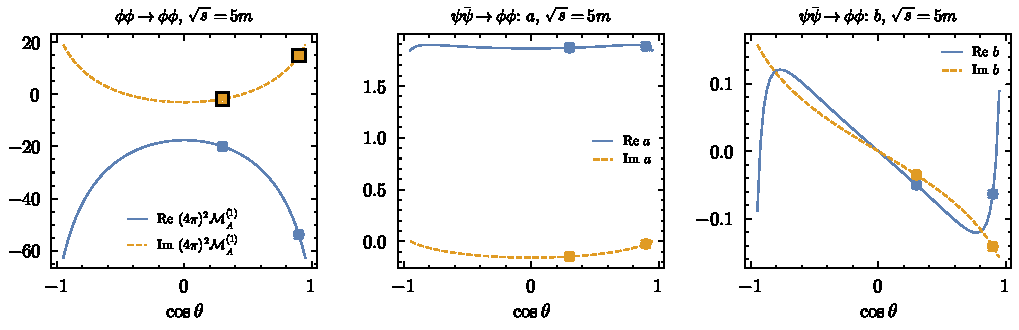
\includegraphics[width=\linewidth]{../figs/scat_d4.pdf}
\caption{$\sqrt s=5m$ での1ループの振幅の角度依存性（$m=\mu=1$、$M=0.7$、$y=\lambda=1$）。左は $\phi\phi\to\phi\phi$ の $(4\pi)^2\mathcal M^{(1)}$、中と右は $\psi\bar\psi\to\phi\phi$ の係数 $a$、$b$（式~\eqref{eq:M1B}）。線は COLLIER で評価したノートの式（実線が実部、破線が虚部）、丸は FeynCalc と Package-X、バツは FormCalc と LoopTools、左の四角はユニタリー性の積分（式~\eqref{eq:unit}）による虚部である。$a$ は $\cos\theta$ について偶、$b$ は奇で、$t\leftrightarrow u$ の対称性を表す。}
\label{fig:scat}
\end{figure}

\paragraph{手順 (5)：S 行列要素と MadLoop。}FeynRules と NLOCT で、場と質量を on-shell で、結合を $\MSbar$ で繰り込む対抗項と、R2 の頂点を求めた。NLOCT の on-shell の対抗項 $\delta Z_\phi$、$2m\,\delta m$、$\delta Z_\psi$、$\delta M$ と、湯川の頂点と4点頂点の対抗項は、\ref{app:scat}、\ref{app:scatB} の自己エネルギーから作った手計算の値と、$1/\epsilon$ の係数も有限部分も数値で30桁一致した。$\delta Z_\psi$ と $\delta M$ は $\Sigma_\psi=\slashed p\Sigma_V+M\Sigma_S$ から $\delta Z_\psi=\Sigma_V+2M^2(\Sigma_V'+\Sigma_S')$、$\delta M=-M(\Sigma_V+\Sigma_S)$（$p^2=M^2$）で、フェルミオンの対抗項に $\gamma^5$ の項は現れなかった。R2 の頂点は $\phi\phi$、$\phi\bar\psi\psi$、$\phi^4$ の3つで、値は $iy^2(6M^2-p^2)/(24\pi^2)$、$y^3\gamma^5/(32\pi^2)$、$\frac54iy^4/\pi^2$ だった。これは、NDR の $D$ 次元の分子と4次元の分子の差として手で導いた値と一致する（\ref{app:bmhv}）。したがって、NLOCT の R2 はノートと同じ NDR の処方に対応する。

続いて、on-shell の対抗項を持つ UFO と、対抗項の極だけを持つ $\MSbar$ の UFO を書き出し、MadLoop で二つの過程の1ループの振幅を計算した。on-shell の UFO の値は S 行列要素（式~\eqref{eq:Mphys}、\eqref{eq:MphysB}）と、$\MSbar$ の UFO の値は外線の補正を除いた振幅（式~\eqref{eq:M1}、\eqref{eq:M1B}）と比べた。比べる量は、始状態のスピンの平均と終状態の同種粒子の因子 $\frac12$ を含む MadLoop の Born と、1ループの有限部分 $2\,\mathrm{Re}(\mathcal M^{(0)*}\mathcal M^{(1)})$ である。$\psi\bar\psi\to\phi\phi$ では、木の振幅との干渉のスピン和が $\sum(\bar v\slashed k_1u)^*\bar vu=2M(t-u)$、$\sum|\bar v\slashed k_1u|^2=2[(t-M^2)(u-M^2)-m^4]$ で決まり、$a$ と $b$ の両方が効く。表~\ref{tab:madloop} に示すように、手順 (4) の6点と、$\sqrt s=5$、$\cos\theta=0.3$ で $\mu_R=m/2,\,2m,\,5m$ とした3点で、Born は丸め誤差の範囲で、有限部分は相対 $2\times10^{-11}$ 以内で一致し、$1/\epsilon$ と $1/\epsilon^2$ の係数は0だった。相対的なずれが最も大きい点は有限部分が打ち消し合って小さい点で、差そのものは $3\times10^{-13}$ 以下である。$\mu_R$ を変えたときの on-shell の値の変化は、$\phi\phi\to\phi\phi$ では $\beta_\lambda$ の三つの項、$\psi\bar\psi\to\phi\phi$ では $-10y^2b^{(0)}$ で、どちらも予想と一致した。これで、式~\eqref{eq:MphysB} の質量のずれと留数の扱いと、手順 (4) の振幅が、MadLoop とも確かめられた。スクリプトは \texttt{generate\_PsYukawa\_NLO.sh}（\texttt{nlo\_renormalize.wl}、\texttt{nlo\_nloct.wl}、\texttt{nlo\_ufo.wl}）、\texttt{run\_madloop\_check.sh}、\texttt{madloop\_numeric.py} である。

\begin{table}[tbp]
\centering\small
\caption{MadLoop と予想の比較（$m=\mu=1$、$M=0.7$、$y=\lambda=1$、各9点の最大）。「図」は MadGraph が生成した Born、ループ、R2、UV の対抗項の図の数である。UV の図の数は、MadGraph が対抗項の結合を $1/\epsilon$ の部分と有限部分、ループの中の粒子ごとに別々に数えたもので、on-shell の対抗項は有限部分を持つので多くなる。対抗項を入れる場所（$\phi\phi\to\phi\phi$ では4点頂点1か所、$\psi\bar\psi\to\phi\phi$ では内線のフェルミオン2か所と湯川の頂点4か所）は二つの処方で同じである。有限部分のずれは予想に対する相対値、$1/\epsilon$ は有限部分に対する比である。}
\label{tab:madloop}
\begin{tabular}{llllll}
\toprule
過程 & 対抗項 & 図（Born、ループ、R2、UV） & Born & 有限部分 & $1/\epsilon$ \\
\midrule
$\phi\phi\to\phi\phi$ & on-shell & 1, 9, 1, 3 & $<10^{-15}$ & $1.5\times10^{-12}$ & $3.7\times10^{-15}$ \\
 & $\MSbar$ & 1, 9, 1, 2 & $<10^{-15}$ & $1.2\times10^{-12}$ & $3.3\times10^{-15}$ \\
$\psi\bar\psi\to\phi\phi$ & on-shell & 2, 11, 4, 20 & $1.1\times10^{-15}$ & $2.1\times10^{-11}$ & $1.3\times10^{-12}$ \\
 & $\MSbar$ & 2, 11, 4, 10 & $1.1\times10^{-15}$ & $1.9\times10^{-11}$ & $3.0\times10^{-12}$ \\
\bottomrule
\end{tabular}
\end{table}

\paragraph{手順 (6)：全断面積。}式~\eqref{eq:sigmatot} の各項を、極質量 $m_{\mathrm p}=1$、$M_{\mathrm p}=0.7$ と $\MSbar$ の $y=\lambda=1$（$\mu=m$）で求めた（単位は GeV）。$\mathcal M_A^{(1)}$ と $a$、$b$ は手順 (4) と同じく COLLIER で求め、式~\eqref{eq:Mphys}、\eqref{eq:MphysB} の変換の項を足して $\cos\theta$ について積分した。$\phi\phi\to\psi\bar\psi$ の被積分関数は、高いエネルギーで $\cos\theta=\pm1$ の近くに $t$、$u$ チャンネルの伝播関数の山を持つ。そこで $\cos\theta$ の区間の半分ずつで山を平らにする変数を使い（\ref{app:sigmatot}）、Gauss--Legendre の24点ずつで積分した。分点を倍にした値との差は相対 $3\times10^{-14}$ 以下だった。同じ分点で MadLoop（on-shell の対抗項、$\mu_R=m$）を走らせて積分すると、表~\ref{tab:xsec} の5つのエネルギーで、$\sigma_{\bar B}^{(0)}$ は相対 $10^{-15}$、$\sigma_A^{(1)}$ は $6\times10^{-11}$、$\sigma_{\bar B}^{(1)}$ は $2\times10^{-10}$ 以内で一致した。$\sigma_A^{(1)}$ のずれが最も大きいのは、$\sigma_A^{(1)}$ が符号を変える $\sqrt s\approx8m$ に近い $10m$ の点である。$\phi\phi\to\psi\bar\psi$ の MadLoop はこの過程の図をそのまま計算するので、時間反転の段階も確かめられた。

$\sigma_3$ のスピン和は、Dirac 表示の行列で式~\eqref{eq:M3} の $\Gamma$ を作り、トレースをとって求めた。これは MadGraph の standalone の出力の行列要素と、求積の分点から選んだ69点で相対 $6\times10^{-14}$ 以内で一致した。位相空間の積分では、$\sum|\mathcal M_3|^2$ を $\psi$ の山と $\bar\psi$ の山に応じて二つに分けた。それぞれ、そのフェルミオンを単独の粒子とし、その角度の山を平らにする変数で、4変数の Gauss--Legendre の求積を行った（\ref{app:sigmatot}）。各変数32点の値と24点の値の差は、$\sqrt s\le5m$ で相対 $2\times10^{-9}$ 以下、$10m$ で $5\times10^{-6}$、$20m$ で $1.4\times10^{-4}$ だった。山を平らにしない求積（$\phi$ を単独の粒子とする）は、$\sqrt s\le5m$ では $5\times10^{-7}$ 以内で一致したが、$20m$ では $1.9\%$ ずれた。独立な検算として、Dalitz の変数と終状態の向きの一様な回転によるモンテカルロ積分（200万点）を行うと、5つのエネルギーで統計誤差の0.7倍以内で一致した。

MadGraph の木の断面積は、$\phi\phi\to\psi\bar\psi$ では $\sqrt s=3m,\,5m,\,10m$ で統計誤差の1.1倍以内で一致した。$\phi\phi\to\phi\psi\bar\psi$ では、MadGraph の値が $0.4\%$、$0.9\%$、$2.4\%$ 小さかった（統計誤差の2.1倍、4.7倍、12倍）。スピン和は一致しているので、ずれは MadGraph の位相空間の積分から来る。$\sqrt s=10m$ で図を分けると、$\lambda y$ の図だけの断面積は $0.02\%$（誤差の0.4倍）で一致し、$y^3$ の図6個だけの断面積は10万事象で $1.8\%$ 小さかった。$\psi$ の向きの分布をモンテカルロ積分（600万点）と比べると、ずれの約4分の1は $|\cos\theta_\psi|>0.999$ の2つのビン（断面積の $1.9\%$）にあり、そこで MadGraph の値は自前の値の $65\%$ と $84\%$ だった。残りのずれは他のビンに広く分かれている（どのビンも誤差の2.5倍以内）。$\phi^3$、$\phi^3+\phi^4$ のノートの $\phi\phi\to\phi\phi\phi$ で見た MadGraph のずれ（$\sqrt s=10m$ で $0.8\%$、$0.3\%$）と同じ向きで、ここでは前方の狭い山のために大きく出たと考えられる。MadGraph の積分の設定を変えても、ずれは残った（\ref{app:details}）。

結果を表~\ref{tab:xsec} と図~\ref{fig:xsec} に示す。全断面積の補正 $\sigma_{\mathrm{tot}}/\sigma_{\mathrm{tot}}^{(0)}-1$ は $\sqrt s\approx2.5m$ で最小の $+7.8\%$ になり、そこから高いエネルギーでは $\sigma_3$ のために増えて、$20m$ で $+22.6\%$ に達する。$\sigma_3/\sigma_{\mathrm{tot}}^{(0)}$ は $\sqrt s=3m$ で $8\%$、$20m$ で $27\%$ である。$\sqrt s=10m$ から $20m$ で、$s\sigma_3$ は1.87倍になり、$s\sigma_{\mathrm{tot}}^{(0)}$（1.39倍）より速く増える。1ループの干渉は、$\phi\phi\to\psi\bar\psi$ では $\sigma_{\bar B}^{(0)}$ の $-8.6\%$（$\sqrt s=2.5m$）から $-2.8\%$（$20m$）である。$\phi\phi\to\phi\phi$ では $\sigma_A^{(0)}$ の $+65\%$（$2.5m$）から $-55\%$（$20m$）まで変わり、$\sqrt s\approx8m$ で符号を変える。$\phi\phi$ の閾値の近くでは $\sigma_A$ が全断面積の大部分を占め（$\sqrt s=2.05m$ で $82\%$）、その1ループの補正（$\sigma_A^{(0)}$ の $+75\%$）のために、全断面積の補正は $+56\%$ になる。$y=\lambda=1$ では、閾値の近くと高いエネルギーで、$y^6$ の次数の補正は小さくない。スクリプトは \texttt{xsec\_collier.f90}（COLLIER）、\texttt{xsec\_mg5.mg5}（MadGraph）、\texttt{run\_xsec\_check.sh}（MadLoop と MadGraph の standalone の出力の準備）、\texttt{xsec\_numeric.py}（積分、MadLoop、比較、図）である。

\begin{table}[tbp]
\centering\footnotesize
\setlength{\tabcolsep}{4pt}
\caption{$\phi\phi$ 散乱の全断面積の内訳（$m_{\mathrm p}=1$、$M_{\mathrm p}=0.7$、$\MSbar$ の $y=\lambda=1$（$\mu=m$）、単位は GeV、断面積は pb）。$\sigma_{\mathrm{tot}}^{(0)}=\sigma_A^{(0)}+\sigma_{\bar B}^{(0)}$ は木の全断面積で、最後の列は $\sigma_{\mathrm{tot}}/\sigma_{\mathrm{tot}}^{(0)}-1$ である。$2\to2$ は Gauss--Legendre の $2\times24$ 点（相対精度 $10^{-13}$）、$\sigma_3$ は各変数32点の求積（相対精度 $10^{-4}$ より良い）による。$\phi\phi\to\phi\psi\bar\psi$ は $\sqrt s>m+2M=2.4m$ で開く。}
\label{tab:xsec}
\begin{tabular}{rrrrrrrrr}
\toprule
$\sqrt s/m$ & $\sigma_A^{(0)}$ & $\sigma_{\bar B}^{(0)}$ & $\sigma_A^{(1)}$ & $\sigma_{\bar B}^{(1)}$ & $\sigma_3$ & $\sigma_{\mathrm{tot}}^{(0)}$ & $\sigma_{\mathrm{tot}}$ & 補正 \\
\midrule
2.5 & $6.197\times10^{5}$ & $2.418\times10^{6}$ & $4.040\times10^{5}$ & $-2.091\times10^{5}$ & $4.303\times10^{4}$ & $3.038\times10^{6}$ & $3.276\times10^{6}$ & $+7.8\%$ \\
3 & $4.304\times10^{5}$ & $3.162\times10^{6}$ & $2.434\times10^{5}$ & $-2.316\times10^{5}$ & $3.020\times10^{5}$ & $3.592\times10^{6}$ & $3.906\times10^{6}$ & $+8.7\%$ \\
5 & $1.549\times10^{5}$ & $2.470\times10^{6}$ & $4.621\times10^{4}$ & $-1.448\times10^{5}$ & $3.666\times10^{5}$ & $2.625\times10^{6}$ & $2.893\times10^{6}$ & $+10.2\%$ \\
10 & $3.873\times10^{4}$ & $1.040\times10^{6}$ & $-4.578\times10^{3}$ & $-4.575\times10^{4}$ & $2.149\times10^{5}$ & $1.079\times10^{6}$ & $1.243\times10^{6}$ & $+15.3\%$ \\
20 & $9.683\times10^{3}$ & $3.657\times10^{5}$ & $-5.326\times10^{3}$ & $-1.042\times10^{4}$ & $1.006\times10^{5}$ & $3.754\times10^{5}$ & $4.603\times10^{5}$ & $+22.6\%$ \\
\bottomrule
\end{tabular}
\end{table}

\begin{figure}[tbp]
\centering
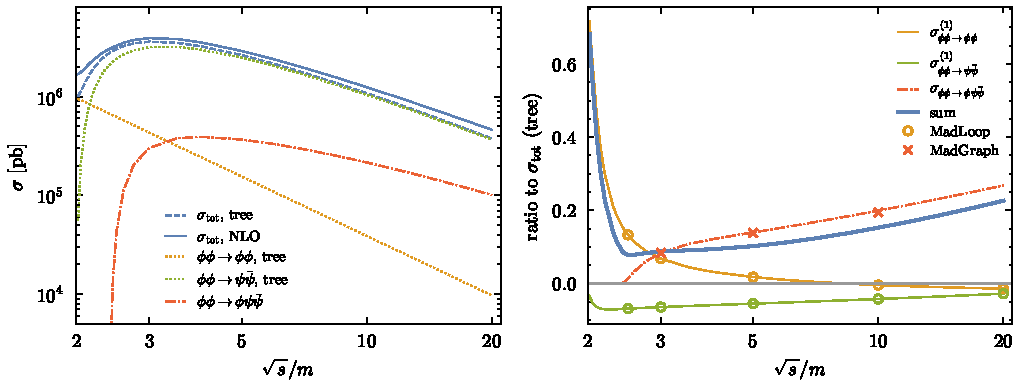
\includegraphics[width=\linewidth]{../figs/xsec_d4.pdf}
\caption{$\phi\phi$ 散乱の全断面積（パラメータは表~\ref{tab:xsec} と同じ）。左は木の全断面積 $\sigma_{\mathrm{tot}}^{(0)}$（破線）、$y^6$ の次数までの $\sigma_{\mathrm{tot}}$（実線）、木の $\sigma_A^{(0)}$、$\sigma_{\bar B}^{(0)}$（点線）と $\sigma_3$（一点鎖線）。右は $y^6$ の次数の各項とその和の $\sigma_{\mathrm{tot}}^{(0)}$ に対する比で、丸は同じ分点で積分した MadLoop の $\sigma_A^{(1)}$、$\sigma_{\bar B}^{(1)}$、バツは MadGraph の $\sigma_3$ である。閾値の近くの立ち上がりは $\sigma_A^{(1)}$ から来る。}
\label{fig:xsec}
\end{figure}

\FloatBarrier
\section{繰り込み群}\label{sec:rg}

この節では、S 行列要素と極質量の $\mu$ 依存から $\beta_\lambda$、$\beta_y$、$\gamma_M$、$\gamma_m$ をツールの数値で読み取り、式~\eqref{eq:rge} と比べる（手順 (7)）。さらに、一般の理論の1ループの公式（文献の値）と比べ、確かめた係数で比 $\lambda/y^2$ の流れを描く。結論を先に述べると、四つの係数は、二つの処方（$\MSbar$ の質量と極質量）の四つのツールすべてで、手計算と相対 $4\times10^{-12}$ 以内で一致した。Machacek と Vaughn の一般の公式は、式~\eqref{eq:rge} の六つの係数を記号として再現した。スクリプトは \texttt{run\_rg\_check.sh} で再実行できる。

\paragraph{手順 (7)：繰り込み群。}物理量は、それをどのパラメータで書いても $\mu$ によらない。質量のパラメータ（$\MSbar$ の $m(\mu)$、$M(\mu)$、または極質量）と $\MSbar$ の結合 $y(\mu)$、$\lambda(\mu)$ で書いた物理量を「木の値（パラメータの関数）$+\,\mathcal Y(\mu)$」とする。$\mathcal Y$ は、パラメータを固定したときの1ループの部分である。木の値をパラメータで微分すると、$\mu$ によらない条件は
\begin{equation}
\mu\frac{\partial\mathcal Y_A}{\partial\mu}=\beta_\lambda,\qquad
\mu\frac{\partial\mathcal Y_a}{\partial\mu}=0,\qquad
\mu\frac{\partial\mathcal Y_b}{\partial\mu}=-(4\pi)^2\Bigl[\frac{2b^{(0)}}{y}\,\beta_y+2My^2\Bigl(\frac{1}{(t-M^2)^2}-\frac{1}{(u-M^2)^2}\Bigr)\gamma_M\Bigr]
\label{eq:rgfit}
\end{equation}
となる（\ref{app:rgfit}）。$\mathcal Y_A$ は $\phi\phi\to\phi\phi$（木の値 $-\lambda$）の、$\mathcal Y_a$、$\mathcal Y_b$ は $\psi\bar\psi\to\phi\phi$ の二つのスピノルの構造（式~\eqref{eq:M1B} と同じく $(4\pi)^2$ を掛けたもの）の1ループの部分である。$\mathcal Y_b$ の右辺の二つの関数は角度依存が違うので、6点から $\beta_y$ と $\gamma_M$ が別々に決まる。二つの場合を調べた。(i) $\MSbar$ の質量。$\mathcal Y_A=\mathcal M_A^{(1)}+4\lambda y^2[B_0^{MM}+m^2B_0^{MM\prime}](m^2)/(4\pi)^2$、$\mathcal Y_a=a_{\mathrm{phys}}$、$\mathcal Y_b=b+(4\pi)^2(\delta R_\psi+\delta R_\phi)b^{(0)}$ で、式~\eqref{eq:MphysB} の質量のずれの項は木の値 $b^{(0)}(M)$ に移る。予想は式~\eqref{eq:rge} の三つの係数である。(ii) 極質量。$\mathcal Y_A$ は (i) と同じ、$(\mathcal Y_a,\mathcal Y_b)=(a_{\mathrm{phys}},b_{\mathrm{phys}})$（式~\eqref{eq:MphysB}）で、$M_{\mathrm p}$ は走らないので予想は $\gamma_M=0$ である。$\phi$ の質量は、どちらの過程でも木の値に運動学を通してしか入らないので、これらの S 行列要素からは $\gamma_m$ が読めない。そこで $\gamma_m$ は、物理量である $\phi$ の極質量 $m_{\mathrm p}^2=m^2+\Sigma_\phi(m^2)$ が $\mu$ によらないことから $\gamma_m=-\mu\,\partial\Sigma_\phi/\partial\mu$ として読む。同じく $M_{\mathrm p}=M[1+\Sigma_V(M^2)+\Sigma_S(M^2)]$ から、$\gamma_M$ をもう一度読む（式~\eqref{eq:mpole}、\eqref{eq:Mpole}）。

数値は、手順 (4) の6点で $\mu=m/2,\,m,\,2m$ として求めた。Package-X と LoopTools は手順 (4) と同じ FeynCalc の振幅と、手順 (3) と同じ自己エネルギーを評価し、COLLIER は式~\eqref{eq:M1}、\eqref{eq:M1B} と極質量の積分を組み立てた。MadLoop は、(i) では極だけの $\MSbar$ の対抗項、(ii) では NLOCT の on-shell の対抗項を使い、$\mu_R=\mu$ として走らせた。$\MSbar$ の MadLoop と FeynCalc、COLLIER の値には、留数と質量のずれの項を Feynman のパラメータの積分から足した。on-shell の MadLoop はそれらを NLOCT の対抗項として含むので、対抗項の $\mu$ 依存の検算にもなる。$\psi\bar\psi\to\phi\phi$ は、MadLoop の有限部分と同じ木の振幅との干渉 $\frac14\mathrm{Re}\sum\mathcal M^{(0)*}\mathcal M^{(1)}$ で当てはめた（\ref{app:rgfit}）。18点の値の COLLIER との相対的なずれは、LoopTools で $1.9\times10^{-13}$、MadLoop で $1.1\times10^{-10}$、Package-X で $9.2\times10^{-10}$ 以内で、on-shell の MadLoop は式~\eqref{eq:Mphys}、\eqref{eq:MphysB} と $3.4\times10^{-11}$ 以内で一致した。虚部は $\mu$ によらず全桁が同じだった。パラメータを固定すると $\mathcal Y$ は $\ln\mu$ の1次式なので、傾きは $\mu=2m$ と $m/2$ の値の差を $2\ln2$ で割って求め、$\mu=m$ の値が両端の平均と一致することを確かめた。FeynCalc の振幅と自己エネルギーの $\mu$ 依存は、Package-X の記号的なスケールで、\ref{app:rgfit} の式と記号としても一致した。

結果を表~\ref{tab:rg} に示す。二つの場合の四つのツールすべてで、$\beta_\lambda$ は相対 $1.2\times10^{-15}$、$\beta_y$ は $2.6\times10^{-13}$、$\gamma_M$ は $3.8\times10^{-12}$ 以内で予想と一致し、(ii) の $\gamma_M$ は $(4\pi)^{-2}$ を単位として $3\times10^{-12}$ 以下だった。$\mathcal Y_a$ の傾きは $5\times10^{-15}$ 以下で0だった。極質量からの $\gamma_m$、$\gamma_M$ は、三つのツールで相対 $9\times10^{-16}$ 以内で一致した。さらに、$\beta_\lambda$ の三つの項を別々に確かめた。COLLIER の $\phi$ の泡の部分の傾きは $3\lambda^2$、フェルミオンの箱の部分は $-48y^4$、on-shell と $\MSbar$ の MadLoop の差（$\phi$ の留数）は $8\lambda y^2$ で、いずれも相対 $10^{-15}$ で一致した。$\phi^3+\phi^4$ のノートと同じく、この一致は数値の精度というより、対抗項、振幅、S 行列要素への変換、各ツールの $\mu$ の約束が整合していることの検算である。ここでは、フェルミオンの質量の走り $\gamma_M$ と、外線のフェルミオンの留数がこの整合に加わる。

\paragraph{一般の公式との比較。}実のスカラー場と2成分のフェルミオンからなる一般の理論の1ループの $\beta$ 関数と異常次元は、Machacek と Vaughn の公式~\cite{mv1,mv2,mv3} で与えられる。質量は、伝播しない「ダミー」のスカラー場との結合とみなして同じ公式から得る~\cite{luo}。Dirac 場を $\psi=(\chi,\eta^\dagger)$ と2成分に分けると、質量は $m_{ij}=M\sigma_1$、擬スカラーの湯川結合は $Y_{ij}=-iy\sigma_1$ と、湯川の行列の位相 $-i$ として現れる。この位相は $Y^\dagger Y$ の形の項には効かず、$Ym^\dagger Y$ とトレースの項の符号だけを変える（\ref{app:rgfit}）。公式に入れると、式~\eqref{eq:rge} の $\beta_y$、$\beta_\lambda$、$\gamma_m$、$\gamma_M$、$\gamma_\phi$、$\gamma_\psi$ の六つがすべて記号として再現された（\texttt{rg\_general.py}）。同じ公式でスカラーの湯川結合（$Y=y\sigma_1$）を調べると、$\gamma_M$ は $5y^2M/(4\pi)^2$ になる。このうち $2y^2M/(4\pi)^2$ はフェルミオンのループのタドポールの項で、それを除いた $3y^2M/(4\pi)^2$ が第~\ref{sec:results} 節で述べたスカラーの湯川結合の値である。擬スカラーではタドポールの項はトレースが0で消え、$Ym^\dagger Y$ の項が符号を変えて $\gamma_M=-y^2M/(4\pi)^2$ になる。質量によらない $\beta_y=5y^3/(4\pi)^2$ と $\beta_\lambda=(3\lambda^2+8\lambda y^2-48y^4)/(4\pi)^2$ は、スカラーの湯川結合の教科書の値~\cite{srednicki} と同じで、第~\ref{sec:results} 節のカイラル回転の議論と合う。

図~\ref{fig:rg} は、$\sqrt s=5m$、$\cos\theta=0.3$ で、(i) のパラメータで書いた $\mathcal M_A$ と $\sum|\mathcal M_B|^2$ の $\mu$ を $m/4$ から $4m$ まで変えたものである。パラメータを固定すると、$\mu=m$ からのずれは最大 $30\%$ と $19\%$ になる。$y$、$\lambda$、$M$ を1ループの解（式~\eqref{eq:rflow} と $M\propto y^{-1/5}$）で走らせると、ずれは $5.5\%$ と $2.8\%$ に縮む。この残りは、木の値を $\ln\mu$ について2次まで展開した項 $\frac12\ddot{\mathcal M}^{(0)}\ln^2(\mu/m)$ である（\ref{app:rgfit}）。その予想値 $-4.98\times10^{-2}$、$+2.51\times10^{-2}$ は、両端の平均 $-5.01\times10^{-2}$、$+2.54\times10^{-2}$ と $\ln^4$ の項の範囲で一致する。残りが $\phi^3+\phi^4$ 理論（$5\times10^{-4}$）より大きいのは、$\beta_\lambda$ がフェルミオンの箱の $-48y^4$ のために大きく、その走りの2次の項も大きいからである。

図~\ref{fig:rgflow} は、確かめた係数による $(y^2,\lambda)$ の流れである。式~\eqref{eq:rflow} の閉じた形は、数値積分と $10^{-12}$ で一致した。半直線 $\lambda=r_\pm y^2$ は流れで保たれる。赤外（$y^2\to0$）では、すべての軌道が $\lambda=r_+y^2$ に沿って原点に向かう。紫外では、$r<r_+$ の軌道は $\lambda=0$ を横切って $\lambda=r_-y^2$ に近づき、$r>r_+$ の軌道は $y$ より先に $\lambda$ の Landau 極に達する。基準点（$\mu=m$ で $y=\lambda=1$）の軌道は、$\mu=19.49m$（$y^2=1.232$）で $\lambda=0$ を横切る。$y$ の Landau 極は $\mu=7.2\times10^6m$ にある。$\lambda$ が0を横切ること自体は物理的な出来事ではない。$\lambda(\mu)$ は $\MSbar$ の結合で、0になるスケールは処方を変えれば $O(1)$ の因子で変わり、S 行列要素は $\mu$ によらない。意味を持つのは、大きな場 $\phi\gg m,M$ での有効ポテンシャルである。繰り込み群で改良すると $V\approx\lambda(\mu\approx\phi)\phi^4/4!$ で、$\lambda<0$ ではこれが負になり、$\phi=0$ は最低エネルギーの状態ではなくなる（偽の真空）。$V$ が負になる場の値そのものは、1ループの補正を含めた結合で決まるので、$19.49m$ とは $O(1)$ の因子で違う。それが問題になるかどうかは真空の崩壊率で決まり、手順 (9)、(10) で調べる。目安として、質量のない理論の bounce の作用 $16\pi^2/|\lambda|$（\ref{app:rgfit}）に走る $\lambda$ を入れると、$\mu=30m$、$100m$、$10^3m$ で $757$、$175$、$56$ である。$\lambda$ は0を過ぎても下がり続けるので、小さい bounce ほど作用が小さい。

\begin{table}[tbp]
\centering\small
\caption{S 行列要素と極質量の $\mu$ 依存から式~\eqref{eq:rgfit} で読み取った係数（$m=1$、$M=0.7$、$y=\lambda=1$、$\mu=m$）。ツールは Package-X、LoopTools、COLLIER、MadLoop（(i) は極だけの $\MSbar$ の対抗項、(ii) は on-shell の対抗項。(ii) は $\MSbar$ の MadLoop に変換の項を足したものも含む）。極質量は MadLoop を除く三つ。「ずれ」はツールの間の最大値で、予想が0でないものは相対的なずれ、(ii) の $\gamma_M$ は $(4\pi)^2|\gamma_M|$ である。}
\label{tab:rg}
\setlength{\tabcolsep}{4pt}
\begin{tabular}{lllll}
\toprule
場合 & 量 & 予想 & 予想の値 & ずれ \\
\midrule
(i) $\MSbar$ の質量 & $\beta_\lambda$ & $(3\lambda^2+8\lambda y^2-48y^4)/(4\pi)^2$ & $-2.3430523717\times10^{-1}$ & $1.2\times10^{-15}$ \\
 & $\beta_y$ & $5y^3/(4\pi)^2$ & $3.1662869888\times10^{-2}$ & $2.6\times10^{-13}$ \\
 & $\gamma_M$ & $-y^2M/(4\pi)^2$ & $-4.4328017844\times10^{-3}$ & $3.8\times10^{-12}$ \\
(ii) 極質量 & $\beta_\lambda$ & 同上 & $-2.3430523717\times10^{-1}$ & $1.2\times10^{-15}$ \\
 & $\beta_y$ & 同上 & $3.1662869888\times10^{-2}$ & $2.6\times10^{-13}$ \\
 & $\gamma_M$ & $0$ & $0$ & $2.7\times10^{-12}$ \\
極質量 & $\gamma_m$ & $(\lambda m^2+4y^2m^2-8y^2M^2)/(4\pi)^2$ & $6.8391798959\times10^{-3}$ & $8.9\times10^{-16}$ \\
 & $\gamma_M$ & $-y^2M/(4\pi)^2$ & $-4.4328017844\times10^{-3}$ & $2.0\times10^{-16}$ \\
\bottomrule
\end{tabular}
\end{table}

\begin{figure}[tbp]
\centering
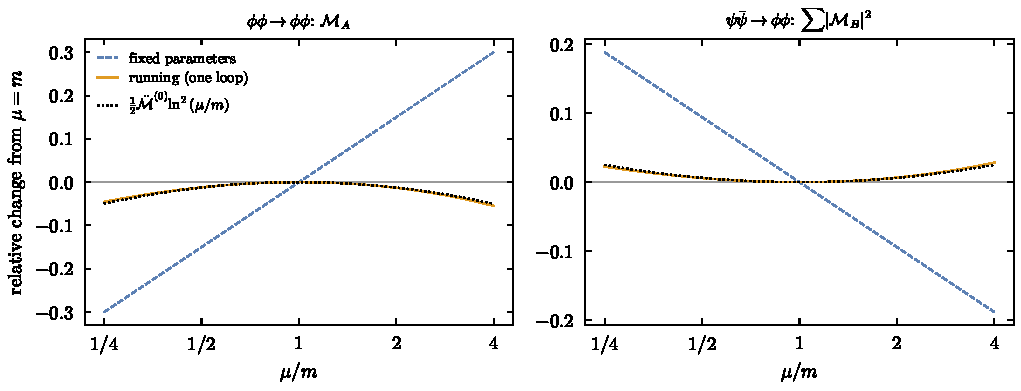
\includegraphics[width=\linewidth]{../figs/rg_d4.pdf}
\caption{$\sqrt s=5m$、$\cos\theta=0.3$ での、$\MSbar$ のパラメータで書いた $\phi\phi\to\phi\phi$ の S 行列要素（左）と $\psi\bar\psi\to\phi\phi$ のスピン和 $\sum|\mathcal M_B|^2$（右、木と1ループの干渉まで）の $\mu$ 依存（$\mu=m$ からの相対的な変化、$\mu=m$ で $m=1$、$M=0.7$、$y=\lambda=1$）。破線はパラメータを固定したもの、実線は $y$、$\lambda$、$M$ を1ループの解で走らせたもの、点線は残りの予想 $\frac12\ddot{\mathcal M}^{(0)}\ln^2(\mu/m)$ である。1ループの部分は COLLIER の値である。}
\label{fig:rg}
\end{figure}

\begin{figure}[tbp]
\centering
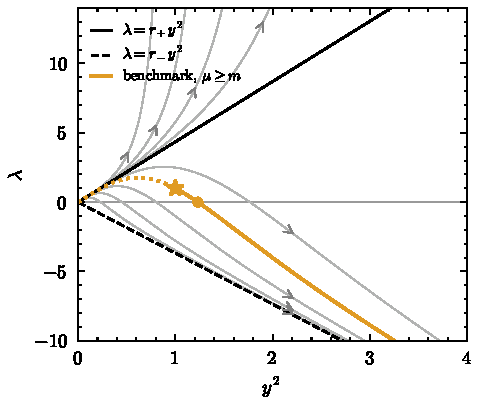
\includegraphics[width=0.55\linewidth]{../figs/rgflow.pdf}
\caption{$(y^2,\lambda)$ の繰り込み群の流れ（1ループ、$\MSbar$）。矢印は紫外（$\mu$ が大きくなる向き）を向く。灰色の線は式~\eqref{eq:rflow} の軌道、黒の実線と破線は流れで保たれる半直線 $\lambda=r_+y^2$ と $\lambda=r_-y^2$、橙の線は基準点（星印、$\mu=m$ で $y=\lambda=1$）を通る軌道（点線は $\mu<m$）、丸は $\lambda=0$ になる点（$\mu=19.49m$）である。}
\label{fig:rgflow}
\end{figure}

\FloatBarrier
\section{摂動論の限界と真空の安定性}\label{sec:pheno}

この節では、この模型の物理の二つの限界を調べる。一つは、結合が大きくなると摂動論とユニタリー性が破れることである。もう一つは、第~\ref{sec:rg} 節で見た $\lambda<0$ による真空の不安定性である。手順は次の三つである。(8) $\phi\phi$ と $\psi\bar\psi$ のヘリシティの状態を合わせた部分波のユニタリー性から、$(y,\lambda)$ の限界を出す。(9) 繰り込み群で改良した有効ポテンシャルで $\lambda<0$ の bounce の作用を求める。(10) フェルミオンの行列式を含む崩壊率の前因子を求め、真空の準安定性の限界を出す。現時点では手順 (8) まで終わっている。結論を先に述べると、木のユニタリー性は、結合を固定すると $y<\sqrt{8\pi/3}=2.89$ と $|\lambda|<16\pi$ を与え、許される領域はほぼこの長方形である。結合の走りを入れて理論を $\sqrt s=E$ まで使うことを求めると、$E=10m$ で $y(m)\le1.94$、$E=100m$ で $y(m)\le1.56$ になる。基準点はこれらを $10^6m$ まで満たすので、基準点を制限するのはユニタリー性ではなく、手順 (9)、(10) の真空の安定性である。スクリプトは \texttt{run\_pw\_check.sh} で再実行できる。

\paragraph{手順 (8)：部分波のユニタリー性。}外線にフェルミオンがあるので、部分波はヘリシティの状態で定義する~\cite{jw}。重心系で $z$ 軸に沿う2体の状態 $|\lambda_1\lambda_2\rangle$（$\lambda=\lambda_1-\lambda_2$）とその回転を使い、
\begin{equation}
a^J_{fi}(s)=\frac{\sqrt{\beta_i\beta_f}\,S_iS_f}{32\pi}\int_{-1}^{1}\!\dd c\;d^J_{\lambda_i\lambda_f}(\theta)\,\mathcal M_{fi}(s,\theta),\qquad
\mathrm{Abs}\,a^J=a^Ja^{J\dagger},\qquad|\mathrm{Re}\,a^J_{(k)}|\le\frac12
\label{eq:pw}
\end{equation}
と定義する（\ref{app:pw}）。$\beta=2|\boldsymbol p|/\sqrt s$、$S=1/\sqrt2$（$\phi\phi$）または1、$a^J_{(k)}$ は行列 $a^J$ の固有値である。$\phi\phi$ の部分波 $a_\ell$ は $\phi^3+\phi^4$ のノートと同じ規約になる。$J=0$ では、$\phi\phi$ と、$\lambda_1=\lambda_2$ の $\psi\bar\psi(++)$、$\psi\bar\psi(--)$ の三つの状態が混ざる。パリティから、$\phi\phi$（$0^+$）は $\psi\bar\psi$ の一つの組み合わせ（${}^3P_0$）とだけ混ざり、もう一つの組み合わせ（${}^1S_0$、$0^-$）は $s$ チャンネルの $\phi$ と結合する。$J=1/2$、$3/2$ では $\psi\phi$ の状態が、$J=1$、$2$ では $\psi\bar\psi$ の4つのヘリシティの状態（$J=2$ では $\phi\phi$ も）が混ざる。木の振幅は Dirac 表示ではなくカイラル表示の行列とヘリシティのスピノルで陽に作り、$\psi\bar\psi\to\phi\phi$、$\psi\bar\psi\to\psi\bar\psi$ のスピン和は手順 (2) の値を全桁で再現した。行列 $a^J$ はエルミートで（$10^{-18}$）、角度の求積は分点を倍にしても $10^{-16}$ しか変わらなかった。

高エネルギーでは、木の部分波は閉じた形になる（\ref{app:pw}）。質量を無視すると、$\psi\bar\psi(\lambda\lambda)\to\phi\phi$ はカイラリティのために0になり、$\phi\phi$ と $\psi\bar\psi(\lambda\lambda)$ の混合は $|a^0|=\sqrt2\,\frac{y^2}{16\pi}\frac{M}{\sqrt s}[\ln(s/M^2)-2]$ のように消える。$\psi\bar\psi\to\psi\bar\psi$ は、$s$ チャンネルが $(++)$、$(--)$ のどの組でも $-y^2$、$t$ チャンネルがヘリシティを反転させる組でだけ $-y^2$ を与え、
\begin{equation*}
a^0\to\mathrm{diag}\Bigl(-\frac{\lambda}{32\pi}\Bigr)\oplus\frac{y^2}{16\pi}\begin{pmatrix}-1&-2\\-2&-1\end{pmatrix},\qquad
a^0_{(k)}\to-\frac{\lambda}{32\pi},\ -\frac{3y^2}{16\pi}\ ({}^1S_0),\ +\frac{y^2}{16\pi}\ ({}^3P_0)
\end{equation*}
となる。$\sqrt s=10^4m$ で、数値の行列の要素はこれらと $2\times10^{-7}$ で、5つの角度のヘリシティの振幅は質量なしの形（\ref{app:pw}）と $4\times10^{-7}$ で一致し、混合は上の式と $4\times10^{-9}$ で一致した（$\ln s$ の係数は $\sqrt s=10^5$〜$10^6m$ で $1.41421$）。$J=1/2$ では二つのヘリシティがともに $-3y^2/(32\pi)$ に近づく。$y=1$ の木の固有値の最大は、$16\pi$ を単位として、$J=0$ が3（$s\to\infty$）、$J=1/2$ が $1.89$（$\sqrt s=4.4m$）、$J=1$ が $0.50$、$J=3/2$ が $0.67$、$J=2$ が $0.91$ で、$J=0$ が最も強い。

限界は三つの基準で求めた（表~\ref{tab:pw}、図~\ref{fig:pw} 上）。
\begin{itemize}
\item (A) 木のユニタリー性：結合を固定して、すべての $s$（$2M<\sqrt s\le10^4m$）と $J\le2$ で $|\mathrm{Re}\,a^J_{(k)}|\le\frac12$。
\item (B) 走る結合での木のユニタリー性：$m\le\mu\le E$ で $y(\mu)$、$\lambda(\mu)$ が (A) の高エネルギーの限界を満たす。
\item (C) 1ループのユニタリー性：$\phi\phi$ を含む要素について、$2m<\sqrt s\le4m$ で $|\mathrm{Re}\,a^0_{\phi\phi,\phi\phi}|\le\frac12$、$|a^0_{\phi\phi,\psi\bar\psi}|\le\frac12$。
\end{itemize}
$a^J=y^2P_J(s)+\lambda Q_J(s)$ は $(y^2,\lambda)$ の1次式なので、(A) の領域は凸で、$(y^2,\lambda)$ の平面の半直線に沿って求まる。(A) は高エネルギーの極限で決まり、$\lambda=0$ では $y^2\le8\pi/3$（${}^1S_0$）、$y=0$ では $|\lambda|\le16\pi$（$\phi\phi$）である。上限は $s\to\infty$ でだけ達し、質量はこれを強めない。領域はほぼ長方形 $y^2\le8\pi/3$、$|\lambda|\le16\pi$ で、角（$|\lambda|\approx16\pi$、$y^2\gtrsim5$）でだけ、$\phi\phi$ と ${}^3P_0$ の混合のために最大 $1.2\%$ 内側に入る（$\sqrt s=14$〜$33m$ で決まる）。$\lambda<0$ の角で縮みが大きいのは、二つの正の固有値 $-\lambda/(32\pi)$ と $y^2/(16\pi)$ が近づき、混合で押し広げられるからである。$y$ の限界は Allwicher らの一般の湯川理論の限界~\cite{allwicher} の、実のスカラーと Dirac フェルミオン1つの場合（$N=1$）の $y^2<8\pi/(2N+1)$ と一致する。彼らの $J=0$ の行列 $\frac{y^2}{16\pi}\bigl(\begin{smallmatrix}-1&2\\2&-1\end{smallmatrix}\bigr)$ とは非対角の符号が違うが、これは $(--)$ の状態の位相の取り方（$|--\rangle\to-|--\rangle$）の違いで、固有値は同じである。$J=1/2$ の高エネルギーの極限の $y^2<16\pi/3$ も一致する。$J=1/2$ では質量の効果で $\sqrt s=4.4m$ の固有値が極限より大きく、結合を固定した限界は $y\le3.65$ になるが、$J=0$ より弱い。質量のない極限では、擬スカラーの結合はカイラル回転でスカラーの結合に移るので（第~\ref{sec:results} 節）、高エネルギーの限界は両者で同じである。$\lambda$ の限界は $\phi^3+\phi^4$ のノートの $16\pi$ と同じである。

(B) では、結合が走るので、限界は理論を使うエネルギー $E$ に依存する。$y$ の条件は閉じた形で $y(m)^2\le(8\pi/3)/[1+\frac{5}{3\pi}\ln(E/m)]$ になり（\ref{app:pw}）、$E=10m$、$100m$ でそれぞれ $y(m)\le1.94$、$1.56$ である。$\lambda$ の上限は、$y=0$ で $\lambda(m)\le16\pi/[1+\frac3\pi\ln(E/m)]$、すなわち $15.7$、$9.3$ で、$y$ が大きいと $-48y^4$ が $\lambda$ の増加を抑えるので少し緩む。$\lambda(m)<0$ の側は、$y$ が小さいと $\lambda$ が0に向かって走るので、$-16\pi$ 近くまで許される。基準点（$\mu=m$ で $y=\lambda=1$）は $E=1.1\times10^6m$ まで (B) を満たす。

(C) では、手順 (4)〜(6) の COLLIER の1ループの振幅を結合の構造（$\lambda^2$、$y^4$、$\lambda y^2$）に分けて S 行列要素（式~\eqref{eq:Mphys}、\eqref{eq:MphysB}）を作り、射影した。$\psi\bar\psi\to\psi\bar\psi$ の1ループは計算していないので、$\phi\phi$ を含む要素だけを使う。射影は、部分波のユニタリー性 $\mathrm{Abs}\,a^{0(1)}_{\phi\phi,i}=(a^{0(0)}a^{0(0)})_{\phi\phi,i}$（$i=\phi\phi$、$\psi\bar\psi(\pm\pm)$）で確かめた。$\phi$ の運動量 $p\ge0.1m$ では相対 $3\times10^{-10}$、閾値のすぐ近く（$p=0.04m$）では両辺がともに小さく $1\times10^{-8}$ で成り立った（図~\ref{fig:pw} 下）。$\mu=m$ では、$\lambda=0$ で $y\le3.79$、$y=1$ で $-71\le\lambda\le48.6$ である。$\mu$ を $m/2$ から $2m$ まで変えると（結合は1ループの解で走らせる）、$y$ の限界は $4.91$ から $2.78$ まで、$\lambda$ の上限は $69.9$ から $43.5$ まで動く。木の限界の近くでは $y^4$ のフェルミオンの箱が大きく、1ループの限界は $\mu$ の選び方に強く依存する。木のユニタリー性の限界は、摂動論が破れ始めるところとほぼ重なり、(C) は (A) より確かな限界にはならない。スクリプトは \texttt{pw\_collier.f90}（COLLIER）と \texttt{pw\_numeric.py}（部分波と限界）である。

\begin{table}[tbp]
\centering\small
\caption{部分波のユニタリー性から求めた限界（$m=1$、$M=0.7$ は極質量、$y$、$\lambda$ は $\MSbar$ の値で、(A) は結合を固定した値、(B)、(C) は $\mu=m$ の値）。(C) の括弧は、$\mu$ を $m/2$ から $2m$ まで変えたときの範囲である。}
\label{tab:pw}
\setlength{\tabcolsep}{4pt}
\begin{tabular}{llll}
\toprule
基準 & 条件 & $y$ の上限 & $\lambda$ の範囲 \\
\midrule
(A) 木、$J=0$ & $|\mathrm{Re}\,a^0_{(k)}|\le\frac12$（$s\to\infty$） & $\sqrt{8\pi/3}=2.894$ & $|\lambda|\le16\pi=50.27$ \\
(A) 木、$J=1/2$ & 同上（$\sqrt s=4.4m$ で最大） & $3.65$（$s\to\infty$ では $\sqrt{16\pi/3}=4.09$） & — \\
(B) $E=10m$ まで & 走る結合で (A) & $1.94$（$\lambda(m)=1$） & $\lambda(m)\le15.7$（$y=0$） \\
(B) $E=100m$ まで & 同上 & $1.56$（$\lambda(m)=1$） & $\lambda(m)\le9.3$（$y=0$） \\
(C) 1ループ、$\mu=m$ & $\phi\phi$ を含む要素 & $3.79$（$2.78$〜$4.91$） & $-71\le\lambda\le48.6$（$y=1$） \\
\bottomrule
\end{tabular}
\end{table}

\begin{figure}[tbp]
\centering
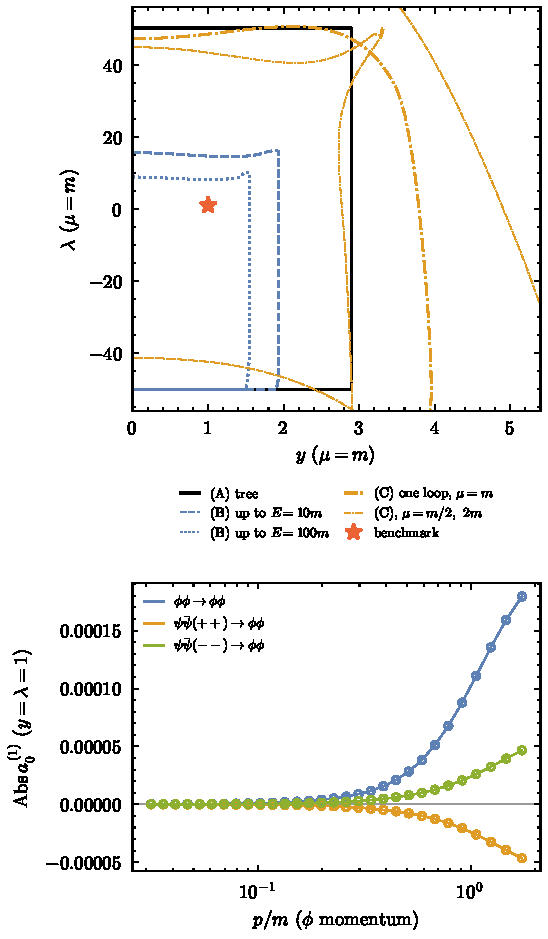
\includegraphics[width=0.55\linewidth]{../figs/pw_d4.pdf}
\caption{部分波のユニタリー性による限界。上：$(y,\lambda)$ の平面（$\mu=m$ の値）。黒の実線は (A) の長方形（角の $1.2\%$ 以下の縮みは見えない）、青の破線と点線は (B) で $E=10m$、$100m$ まで求めたもの、橙の一点鎖線は (C)（太線が $\mu=m$、細線が $\mu=m/2$ と $2m$）の境界で、それぞれ境界の内側（$y$ が小さい側）が許される。星印は基準点である。下：部分波ごとのユニタリー性（$y=\lambda=1$、$\mu=m$）。線は $\phi\phi$ を含む要素の $\mathrm{Abs}\,a^{0(1)}$、白丸は木の積 $(a^{0(0)}a^{0(0)})_{\phi\phi,i}$。横軸は $\phi$ の運動量 $p$（$\sqrt s=2\sqrt{m^2+p^2}$）。}
\label{fig:pw}
\end{figure}

\FloatBarrier
\section{議論と今後}\label{sec:discussion}

\paragraph{手計算で分かったこと。}フェルミオンを入れたことで、スカラー理論にはなかった三つの特徴が現れた。一つ目は、閉じたフェルミオンのループの符号 $-1$ で、これが $\delta_\phi<0$ と $\beta_\lambda$ の $-48y^4$ を与える。二つ目は、$\gamma^5$ がフェルミオンの伝播関数の質量の項の符号を変えることで、$\delta_M$ と $\gamma_M$ の符号がスカラーの湯川結合と逆になる。三つ目は、フェルミオンの箱の図の簡単さで、トレースを分母で書き直すと、テンソル積分を経ずに $B_0$、$C_0$、$D_0$ だけで書ける。物理としては、比 $\lambda/y^2$ の流れが1ループで解析的に解け、$\lambda$ が負になる尺度か、$\lambda$ が発散する尺度のどちらかが、$y$ の Landau 極より手前に必ず現れる。

\paragraph{今後。}次は手順 (9) で、繰り込み群で改良した有効ポテンシャルで $\lambda$ が負になる尺度を求め、$\lambda<0$ の bounce の作用を求める。

\appendix

\section{Feynman 則と対称性因子の導出}\label{app:rules}

\paragraph{伝播関数。}$\phi$ の伝播関数 $i/(p^2-m^2+i0)$ の導出は $\phi^3$ のノート~\cite{phi3note} の付録~A と同じである。$\psi$ の運動項 $\bar\psi(i\slashed\partial-M)\psi$ は、運動量空間（$\psi\propto e^{-ip\cdot x}$）で $\bar\psi(\slashed p-M)\psi$ となる。伝播関数はその逆行列の $i$ 倍で、$(\slashed p-M)(\slashed p+M)=\slashed p\slashed p-M^2=p^2-M^2$ から $i(\slashed p-M)^{-1}=i(\slashed p+M)/(p^2-M^2+i0)$ である。

\paragraph{頂点と対抗項。}頂点の因子は「$i\times(\mathcal{L}_{\mathrm{int}}$ の係数$)\times($同種の場の付け方の数$)$」である。湯川の項 $-iy\mu^\epsilon\phi\bar\psi\gamma^5\psi$ では、$\phi$、$\bar\psi$、$\psi$ はどれも1つずつで付け方は1通りなので、頂点は $i\cdot(-iy\mu^\epsilon\gamma^5)=y\mu^\epsilon\gamma^5$ である。$\gamma^5$ はスピンの添字を持つ行列で、フェルミオンの線に沿って伝播関数と並べて掛ける。4点頂点 $-i\lambda\mu^{2\epsilon}$ の導出は $\phi^3+\phi^4$ のノート~\cite{phi34note} の付録~A と同じである。対抗項も同じ規則に従う。$\frac12\delta_\phi(\partial\phi)^2-\frac12\delta_m\phi^2$ は、2本の線の付け方2通りが $\frac12$ を打ち消して $i(\delta_\phi p^2-\delta_m)$ になる。$\delta_\psi\bar\psi i\slashed\partial\psi-\delta_M\bar\psi\psi$ は運動量空間で $\bar\psi(\delta_\psi\slashed p-\delta_M)\psi$ なので $i(\delta_\psi\slashed p-\delta_M)$、湯川の対抗項は $i\cdot(-i\delta_y\mu^\epsilon\gamma^5)=\delta_y\mu^\epsilon\gamma^5$、4点の対抗項は $-i\delta_\lambda\mu^{2\epsilon}$ である。

\paragraph{閉じたフェルミオンのループ。}湯川の頂点2つを結ぶループを例にとる。$\langle(\bar\psi\Gamma\psi)_x(\bar\psi\Gamma\psi)_y\rangle$（$\Gamma=\gamma^5$）を成分で書くと $\bar\psi_a(x)\Gamma_{ab}\psi_b(x)\,\bar\psi_c(y)\Gamma_{cd}\psi_d(y)$ で、縮約 $\psi_b(x)\bar\psi_c(y)=S_{bc}(x-y)$ と $\psi_d(y)\bar\psi_a(x)=S_{da}(y-x)$ をとる。後者を作るには、$\psi_d(y)$ を $\bar\psi_a(x)$ の左まで動かす必要がある。$\psi_d$ は Grassmann 数の $\bar\psi_c$、$\psi_b$、$\bar\psi_a$ の3つを通り抜けるので、符号 $(-1)^3=-1$ が付く。こうして $-\Gamma_{ab}S_{bc}\Gamma_{cd}S_{da}=-\mathrm{tr}[\Gamma S(x-y)\Gamma S(y-x)]$ となる。頂点が $n$ 個のループでも、最後の $\psi$ を最初の $\bar\psi$ の左に動かすとき、奇数個（$2n-1$ 個）の Grassmann 数を通り抜けるので、符号はいつも $-1$ で、添字はトレースになる。

\paragraph{対称性因子の数え方。}図の値は、$\langle\cdots\frac{1}{n!}(i\int\mathcal{L}_{\mathrm{int}})^n\rangle$ の Wick の縮約のうち、その図を与えるものの数を、頂点の係数とともに数えて決める。同じ種類の頂点が $n$ 個あると $1/n!$ が付くが、どの頂点をどこに置くかの入れ替え $n!$ と打ち消す。湯川の頂点の係数（$i$ と $\mu$ の因子を除く）は $-iy\gamma^5$ で、組み合わせの因子を持たない。

(a) $\phi$ の自己エネルギーのフェルミオンのループ。湯川の頂点2つの $1/2!$ は、頂点の入れ替えの2と打ち消す。外の $\phi$ を頂点 $x$ と $y$ の $\phi$ に付ける方法は1通り、$\psi(x)\bar\psi(y)$ と $\psi(y)\bar\psi(x)$ の縮約も1通りである。よって対称性因子は1である。スカラーの泡（$\phi^3$ 理論の $1/2$）と違うのは、二つのフェルミオンの内線が、フェルミオン数の流れの向き（$x\to y$ と $y\to x$）で区別されるからである。(b) 4点頂点のタドポール型の図は $\phi^3+\phi^4$ のノートの (c) と同じで $1/2$ である。

(c) $\psi$ の自己エネルギー。湯川の頂点2つの $1/2!$ は入れ替えと打ち消す。入ってくる $\psi$ を一方の頂点の $\bar\psi$ に、出ていく $\bar\psi$ を他方の頂点の $\psi$ に付ける方法は1通りで、残りの $\psi\bar\psi$ と $\phi\phi$ の縮約もそれぞれ1通りである。よって1である。(d) 湯川の頂点の補正も同様に、頂点3つの $1/3!$ が入れ替えの $3!$ と打ち消し、残りの縮約は1通りなので1である。(e) $\lambda^2$ の泡は $\phi^3+\phi^4$ のノートの (f) と同じで $1/2$ である。

(f) フェルミオンの箱。湯川の頂点4つの $1/4!$ は、4本の外の $\phi$ を4つの頂点に割り当てる方法 $4!$ 通りと打ち消す。4つの頂点を1本の向きのあるフェルミオンのループで結ぶ縮約は、頂点1から出発して残り3つを訪れる順序の数 $3!=6$ 通りある。それぞれが一つの図で、対称性因子は1である。6つは、ループの向きだけが逆の2つずつ、すなわち外線の巡回の順序が同じ3組に分かれる。向きが逆の二つの図の値が等しいことは\ref{app:gamma5} で示す。

\section{次元とべき数え上げ}\label{app:counting}

\paragraph{次元。}$D$ 次元の作用は無次元なので、$\mathcal{L}$ の質量次元は $D$ である。運動項から $\phi$ の質量次元は $(D-2)/2=1-\epsilon$、$\psi$ の質量次元は $(D-1)/2=\frac32-\epsilon$ である。湯川の項の係数の質量次元は $D-(1-\epsilon)-2(\frac32-\epsilon)=(4-2\epsilon)-4+3\epsilon=\epsilon$、$\phi^4$ の係数の質量次元は $D-4(1-\epsilon)=2\epsilon$ である。そこで、無次元の $y$ と $\lambda$ を使って、係数を $y\mu^\epsilon$、$\lambda\mu^{2\epsilon}$ と書く。

\paragraph{発散次数。}ループ $L$ 個、$\phi$ の内線 $I_\phi$ 本、フェルミオンの内線 $I_\psi$ 本の図では、ループ運動量の積分が $4L$、$\phi$ の伝播関数が $-2$、フェルミオンの伝播関数が $-1$（分子の $\slashed k$ のため）の次数を与えるので、$\omega=4L-2I_\phi-I_\psi$ である。湯川の頂点 $V_y$ 個、4点頂点 $V_4$ 個とすると $L=I_\phi+I_\psi-V_y-V_4+1$ である。線の端の数を場ごとに数えると、$\phi$ では $V_y+4V_4=E_\phi+2I_\phi$、フェルミオンでは $2V_y=E_\psi+2I_\psi$ である。よって
\begin{equation*}
\begin{aligned}
\omega&=4(I_\phi+I_\psi-V_y-V_4+1)-2I_\phi-I_\psi=2I_\phi+3I_\psi-4V_y-4V_4+4\\
&=(V_y+4V_4-E_\phi)+\Bigl(3V_y-\frac32E_\psi\Bigr)-4V_y-4V_4+4=4-E_\phi-\frac32E_\psi
\end{aligned}
\end{equation*}
となり、式~\eqref{eq:omega} を得る。$E_\psi$ は偶数なので、$\omega\ge0$ となるのは $E_\psi=0$ で $E_\phi\le4$、$E_\psi=2$ で $E_\phi\le1$ の場合だけである。

\section{$\gamma^5$、トレース、パリティ}\label{app:gamma5}

\paragraph{$\gamma^5$ の処方。}NDR では、$D$ 次元で $\{\gamma^5,\gamma^\mu\}=0$、$(\gamma^5)^2=1$ とする。これから、任意のベクトル $a$ と数 $M$ について $\gamma^5(\slashed a+M)\gamma^5=-\slashed a\gamma^5\gamma^5+M=-\slashed a+M$ である。トレースは $\mathrm{tr}\,1=4$、奇数個の $\gamma^\mu$ のトレースは0、$\mathrm{tr}[\slashed a\slashed b]=4a\cdot b$、$\mathrm{tr}[\slashed a\slashed b\slashed c\slashed d]=4[(a\cdot b)(c\cdot d)-(a\cdot c)(b\cdot d)+(a\cdot d)(b\cdot c)]$ である。$\gamma^5$ を偶数個含むトレースは、反可換性で $\gamma^5$ を隣り合わせて $(\gamma^5)^2=1$ で消せるので、$\gamma^5$ を含まないトレースに帰着し、曖昧さはない。図 (a)、(c)、(d)、(f) はすべてこの型である（(c) と (d) はトレースではなく開いたフェルミオンの線だが、同じく反可換性だけで整理できる）。

\paragraph{奇数個の $\gamma^5$ を含むトレース。}図 (g) のトレースは $-\mathrm{tr}[\gamma^5\,i(\slashed k+M)]$ で、$\mathrm{tr}[\gamma^5]=0$ と $\mathrm{tr}[\gamma^5\gamma^\mu]=0$ から0である。図 (h) では、$\gamma^5$ を3つ含むトレースを反可換性で $\pm\mathrm{tr}[\gamma^5(\slashed a+M)(\slashed b+M)(\slashed c+M)]$ の形にでき、展開すると $\gamma^5$ と3個以下の $\gamma^\mu$ のトレースだけが残る。4次元ではそれらはすべて0である（0でない最小のものは $\mathrm{tr}[\gamma^5\gamma^\mu\gamma^\nu\gamma^\rho\gamma^\sigma]\propto\epsilon^{\mu\nu\rho\sigma}$）。$D$ 次元の NDR では $\gamma^5$ を含むトレースの値は一般に曖昧だが、ループ積分の後に残る独立なベクトルは外線の運動量2つだけで、$\epsilon^{\mu\nu\rho\sigma}$ を4つの独立なベクトルで縮約した量は作れない。したがって (h) はどの処方でも0である。

\paragraph{エルミート性。}$(\bar\psi i\gamma^5\psi)^\dagger=-i\psi^\dagger\gamma^{5\dagger}\gamma^{0\dagger}\psi=-i\psi^\dagger\gamma^5\gamma^0\psi=i\psi^\dagger\gamma^0\gamma^5\psi=\bar\psi i\gamma^5\psi$ である（$\gamma^{5\dagger}=\gamma^5$、$\gamma^{0\dagger}=\gamma^0$、$\gamma^5\gamma^0=-\gamma^0\gamma^5$ を使った）。

\paragraph{パリティ。}$\psi\to\gamma^0\psi$ のとき $\bar\psi=\psi^\dagger\gamma^0\to\psi^\dagger\gamma^0\gamma^0=\bar\psi\gamma^0$ なので、$\bar\psi\psi\to\bar\psi\gamma^0\gamma^0\psi=\bar\psi\psi$、$\bar\psi i\gamma^5\psi\to\bar\psi\gamma^0i\gamma^5\gamma^0\psi=-\bar\psi i\gamma^5\psi$ である。運動項は $\boldsymbol x\to-\boldsymbol x$ とあわせて不変である。したがって、$\phi\to-\phi$ とあわせると $\phi\bar\psi i\gamma^5\psi$ と $\phi^2$、$\phi^4$ は不変で、$\phi$、$\phi^3$、$\phi\bar\psi\psi$、$\bar\psi i\gamma^5\psi$ は符号を変える。正則化（次元正則化と、1ループの NDR）がこの対称性を保つので、後者の項は対抗項としても要らない。

\paragraph{ループの向きと荷電共役。}荷電共役の行列 $C$ は $C^{-1}\gamma^\mu C=-(\gamma^\mu)^T$、$C^{-1}\gamma^5C=(\gamma^5)^T$ を満たす。よって $(\slashed k+M)^T=C^{-1}(-\slashed k+M)C$ である。$n$ 個の湯川の頂点を持つループのトレースを転置すると
\begin{equation*}
\mathrm{tr}[\gamma^5(\slashed k_1+M)\gamma^5(\slashed k_2+M)\cdots\gamma^5(\slashed k_n+M)]
=\mathrm{tr}[(-\slashed k_n+M)\gamma^5\cdots(-\slashed k_2+M)\gamma^5(-\slashed k_1+M)\gamma^5]
\end{equation*}
となる（$\mathrm{tr}X^T=\mathrm{tr}X$、$C$ と $C^{-1}$ はトレースの中で打ち消す）。右辺は、頂点を逆の順に回り、各伝播関数の運動量の符号を変えたもの、すなわち向きが逆のループのトレースである。分母 $D_M(k_i)$ は $k_i\to-k_i$ で不変なので、向きが逆の二つの図は等しい。ベクトルの頂点 $\gamma^\mu$ なら頂点ごとに $-1$ が付いて Furry の定理になるが、$\gamma^5$ には付かない。

\paragraph{カイラル回転。}$\psi\to e^{i\theta\gamma^5}\psi$ のとき $\bar\psi\to\psi^\dagger e^{-i\theta\gamma^5}\gamma^0=\bar\psi e^{i\theta\gamma^5}$ である。運動項は $\bar\psi e^{i\theta\gamma^5}\gamma^\mu e^{i\theta\gamma^5}\psi=\bar\psi\gamma^\mu e^{-i\theta\gamma^5}e^{i\theta\gamma^5}\psi=\bar\psi\gamma^\mu\psi$ で不変で、$\bar\psi\psi\to\bar\psi e^{2i\theta\gamma^5}\psi=\cos2\theta\,\bar\psi\psi+\sin2\theta\,\bar\psi i\gamma^5\psi$ である。$\theta=\pi/4$ とすると $\bar\psi\psi\to\bar\psi i\gamma^5\psi$ となり、$M=0$ のスカラーの湯川理論 $-y\phi\bar\psi\psi$ は本模型の $M=0$ の場合に移る。したがって、質量によらない量（$\beta_y$、$\beta_\lambda$、$\gamma_\phi$、$\gamma_\psi$）は両者で等しい。質量の項 $-M\bar\psi\psi$ は回転で $-M\bar\psi i\gamma^5\psi$ に移るので、$\gamma_M$ と $\gamma_m$ の $M^2$ の項は両者で異なりうる。

\section{1PI 関数と対抗項の導出}\label{app:ren}

\paragraph{積分の規約。}$\phi^3$ のノートの付録~C と同じく、$\overline{\mathrm{MS}}$ では
\begin{equation*}
\mu^{2\epsilon}I_1^a=\frac{i}{(4\pi)^2}\bigl[m_a^2\Delta_{\mathrm{UV}}+A_0(m_a^2)\bigr],\qquad
\mu^{2\epsilon}I_2^{ab}(p^2)=\frac{i}{(4\pi)^2}\bigl[\Delta_{\mathrm{UV}}+B_0^{ab}(p^2)\bigr]
\end{equation*}
で、$A_0(m^2)=m^2(1-\ln(m^2/\mu^2))$、$B_0^{ab}(p^2)=-\int_0^1\dd x\,\ln[\Delta_x/\mu^2]$、$\Delta_x=xm_b^2+(1-x)m_a^2-x(1-x)p^2-i0$ である。ベクトルの2点積分は、Feynman のパラメータで分母を $[(k+xp)^2-\Delta_x]^2$ とまとめ、$k=\ell-xp$ とずらすと、$\ell^\mu$ の奇関数の項が消えて
\begin{equation*}
\mu^{2\epsilon}\int\frac{\dd^Dk}{(2\pi)^D}\frac{k^\mu}{D_a(k)D_b(k+p)}=-p^\mu\int_0^1\dd x\,x\,\mu^{2\epsilon}\int\frac{\dd^D\ell}{(2\pi)^D}\frac{1}{(\ell^2-\Delta_x)^2}
=\frac{i}{(4\pi)^2}\,p^\mu\Bigl[-\frac12\Delta_{\mathrm{UV}}+B_1^{ab}(p^2)\Bigr]
\end{equation*}
となる。$B_1^{ab}(p^2)=\int_0^1\dd x\,x\ln[\Delta_x/\mu^2]$ で、LoopTools の $B_1(p^2,m_a^2,m_b^2)$ の $\Delta=0$ の値である。3点と4点の積分は、LoopTools の規約で $\int\dd^Dk\,\{1,k^\mu\}/(D_{a}(k)D_{b}(k+r_1)D_{c}(k+r_2))=\frac{i}{(4\pi)^2}\{C_0,\ r_1^\mu C_1+r_2^\mu C_2\}$（$\mu^{2\epsilon}$ を含む、引数は $(r_1^2,(r_2-r_1)^2,r_2^2;m_a^2,m_b^2,m_c^2)$）と、同様の $D_0$ で表す。$C_0$、$C_i$、$D_0$ は有限である。

\paragraph{$V_\phi$。}図 (a) は、ループの $-1$、頂点2つ、伝播関数2本から
\begin{equation*}
-\int\frac{\dd^Dk}{(2\pi)^D}\mathrm{tr}\Bigl[y\mu^\epsilon\gamma^5\,\frac{i(\slashed k+M)}{D_M(k)}\,y\mu^\epsilon\gamma^5\,\frac{i(\slashed k+\slashed p+M)}{D_M(k+p)}\Bigr]
=y^2\mu^{2\epsilon}\int\frac{\dd^Dk}{(2\pi)^D}\frac{\mathrm{tr}[(-\slashed k+M)(\slashed k+\slashed p+M)]}{D_M(k)D_M(k+p)}
\end{equation*}
である（$-i^2=1$ と $\gamma^5(\slashed k+M)\gamma^5=-\slashed k+M$）。トレースは $-4k\cdot(k+p)+4M^2$ で、$k\cdot(k+p)=\frac12[D_M(k)+D_M(k+p)+2M^2-p^2]$ を使うと $2p^2-2D_M(k)-2D_M(k+p)$ になる。$D_M(k)$ と $D_M(k+p)$ はそれぞれ一方の伝播関数を消し、積分変数をずらすとどちらも $I_1^M$ を与える。よって (a) $=2y^2\mu^{2\epsilon}[p^2I_2^{MM}(p^2)-2I_1^M]$ である。図 (b) は $\phi^3+\phi^4$ のノートと同じく $\frac\lambda2\mu^{2\epsilon}I_1^m$ である。上の積分の展開を入れると
\begin{equation*}
V_\phi=\frac{i}{(4\pi)^2}\Bigl[2y^2\bigl(p^2(\Delta_{\mathrm{UV}}+B_0^{MM})-2(M^2\Delta_{\mathrm{UV}}+A_0(M^2))\bigr)+\frac\lambda2\bigl(m^2\Delta_{\mathrm{UV}}+A_0(m^2)\bigr)\Bigr]+i(\delta_\phi p^2-\delta_m)
\end{equation*}
で、$\Delta_{\mathrm{UV}}$ の係数が $p^2$ によらず0になる条件は $2y^2/(4\pi)^2+\delta_\phi/\Delta_{\mathrm{UV}}=0$ と $(-4y^2M^2+\frac\lambda2m^2)/(4\pi)^2-\delta_m/\Delta_{\mathrm{UV}}=0$ である。これが式~\eqref{eq:ct} の $\delta_\phi$、$\delta_m$ で、残りが式~\eqref{eq:VR} の $V_\phi$ である。

\paragraph{$V_\psi$。}入ってくるフェルミオンの運動量を $p$、ループのフェルミオンの運動量を $k$ とすると、$\phi$ の内線の運動量は $p-k$ で、
\begin{equation*}
\int\frac{\dd^Dk}{(2\pi)^D}\,y\mu^\epsilon\gamma^5\,\frac{i(\slashed k+M)}{D_M(k)}\,y\mu^\epsilon\gamma^5\,\frac{i}{D_m(k-p)}
=-y^2\mu^{2\epsilon}\int\frac{\dd^Dk}{(2\pi)^D}\frac{-\slashed k+M}{D_M(k)D_m(k-p)}
\end{equation*}
となり、式~\eqref{eq:V} の $V_\psi$ を得る。$k\to-k$ とすると分母は $D_M(k)D_m(k+p)$ になり、上のベクトルの積分の規約（$a=M$、$b=m$）が使えて、$\mu^{2\epsilon}\int k^\mu/(D_M(k)D_m(k-p))=-\frac{i}{(4\pi)^2}p^\mu[-\frac12\Delta_{\mathrm{UV}}+B_1^{Mm}]$ である。よって
\begin{equation*}
V_\psi=\frac{iy^2}{(4\pi)^2}\Bigl[-\slashed p\Bigl(-\frac12\Delta_{\mathrm{UV}}+B_1^{Mm}\Bigr)-M\bigl(\Delta_{\mathrm{UV}}+B_0^{Mm}\bigr)\Bigr]+i(\delta_\psi\slashed p-\delta_M)
\end{equation*}
で、極が消える条件 $y^2/(2(4\pi)^2)+\delta_\psi/\Delta_{\mathrm{UV}}=0$、$-y^2M/(4\pi)^2-\delta_M/\Delta_{\mathrm{UV}}=0$ から式~\eqref{eq:ct} の $\delta_\psi$、$\delta_M$ を得る。

\paragraph{$V_y$。}フェルミオンの線に沿って、出ていく側から書く。入ってくるフェルミオン（運動量 $p$）が $\phi$ の内線（運動量 $p-k$）を出して運動量 $k$ になり、外の $\phi$（運動量 $q$）を吸って $k+q$ になり、$\phi$ の内線を吸って $p'=p+q$ で出ていく。値は
\begin{equation*}
\int\frac{\dd^Dk}{(2\pi)^D}\,y\gamma^5\frac{i(\slashed k+\slashed q+M)}{D_M(k+q)}\,y\gamma^5\frac{i(\slashed k+M)}{D_M(k)}\,y\gamma^5\,\frac{i}{D_m(k-p)}\,\mu^{3\epsilon}
\end{equation*}
で、$i^3=-i$ と $\gamma^5(\slashed k+\slashed q+M)\gamma^5=M-\slashed k-\slashed q$ から、分子は $-iy^3(M-\slashed k-\slashed q)(M+\slashed k)\gamma^5$ になる。積を展開すると $M^2+M\slashed k-M\slashed k-\slashed k\slashed k-M\slashed q-\slashed q\slashed k=M^2-k^2-M\slashed q-\slashed q\slashed k$ で、式~\eqref{eq:V} の $V_y$ を得る。$M^2-k^2=-D_M(k)$ は伝播関数 $D_M(k)$ を消し、残る $\int1/(D_M(k+q)D_m(k-p))$ は運動量の差 $(k+q)-(k-p)=p'$ の2点積分 $I_2^{Mm}(p'^2)$ である。残りの2項は3点積分で、上の規約で $r_1=q$、$r_2=-p$、$(a,b,c)=(M,M,m)$ とすると、$\mu^{2\epsilon}\int k^\mu/(\cdots)=\frac{i}{(4\pi)^2}(q^\mu C_1-p^\mu C_2)$ なので、$\slashed q\slashed k\to\frac{i}{(4\pi)^2}(q^2C_1-\slashed q\slashed pC_2)$ である。まとめると
\begin{equation*}
V_y=-iy^3\cdot\frac{i}{(4\pi)^2}\Bigl[-\bigl(\Delta_{\mathrm{UV}}+B_0^{Mm}(p'^2)\bigr)-M\slashed q\,C_0-q^2C_1+\slashed q\slashed p\,C_2\Bigr]\gamma^5+\delta_y\gamma^5
\end{equation*}
で、$\Delta_{\mathrm{UV}}$ の項は $-y^3\Delta_{\mathrm{UV}}\gamma^5/(4\pi)^2$ である。これを打ち消す $\delta_y=y^3\Delta_{\mathrm{UV}}/(4\pi)^2$ が式~\eqref{eq:ct} で、残りが式~\eqref{eq:VR} の $V_y$ である。$M^2-k^2$ の代わりに $M^2-(k+q)^2$ を作るように整理すると、$B_0^{Mm}(p^2)$ を含む別の形になる。二つは PaVe 関数の恒等式で移り合う。

\paragraph{$V_4$ の泡。}$\lambda^2$ の泡は $\phi^3+\phi^4$ のノートと同じで $\frac{\lambda^2}{2}\sum_xI_2^{mm}(x)$、極は $\frac{3\lambda^2}{2}\frac{i}{(4\pi)^2}\Delta_{\mathrm{UV}}$ である。

\paragraph{フェルミオンの箱。}一つの図は、ループの $-1$、頂点4つ、伝播関数4本の $i^4=1$ から $-y^4\mu^{4\epsilon}\int\mathrm{tr}[\gamma^5(\slashed k_1+M)\gamma^5(\slashed k_2+M)\gamma^5(\slashed k_3+M)\gamma^5(\slashed k_4+M)]/(D_1D_2D_3D_4)$ である（$D_i\equiv D_M(k_i)$）。1番目と3番目の伝播関数の $\gamma^5$ を挟む組を $\gamma^5(\slashed k+M)\gamma^5=M-\slashed k$ で整理すると、トレースは $T=\mathrm{tr}[(M-\slashed k_1)(M+\slashed k_2)(M-\slashed k_3)(M+\slashed k_4)]$ になる。展開すると、$\gamma$ 行列0個の項 $4M^4$、2個の項 $4M^2\sum_{i<j}\sigma_{ij}\,k_i\cdot k_j$（$\sigma_{ij}$ は $k_i$、$k_j$ の前の符号の積で、$\sigma_{12}=\sigma_{14}=\sigma_{23}=\sigma_{34}=-1$、$\sigma_{13}=\sigma_{24}=+1$）、4個の項 $4[(k_1\cdot k_2)(k_3\cdot k_4)-(k_1\cdot k_3)(k_2\cdot k_4)+(k_1\cdot k_4)(k_2\cdot k_3)]$ である。

$s_{ij}\equiv(k_i-k_j)^2$ と置く。$s_{ij}$ は外線の運動量の和の2乗で、$k_i\cdot k_j=\frac12(D_i+D_j)+a_{ij}$、$a_{ij}\equiv M^2-\frac12s_{ij}$ である。これを入れて $D_i$ について整理する。2次の項は、4個の項から $\frac14[(D_1+D_2)(D_3+D_4)-(D_1+D_3)(D_2+D_4)+(D_1+D_4)(D_2+D_3)]=\frac12(D_1D_3+D_2D_4)$ だけが残る。1次の項は、2個の項から $M^2\sum\sigma_{ij}\frac12(D_i+D_j)=-\frac12M^2\sum_iD_i$、4個の項から $D_1$ の係数 $\frac12(a_{34}-a_{24}+a_{23})$（$D_2$、$D_3$、$D_4$ も同様）が来て、合わせると $D_1$ の係数は $\frac12(a_{34}-a_{24}+a_{23}-M^2)=\frac14(s_{24}-s_{23}-s_{34})$ となる。定数項は
\begin{equation*}
M^4+M^2\sum_{i<j}\sigma_{ij}a_{ij}+(a_{12}a_{34}-a_{13}a_{24}+a_{14}a_{23})
\end{equation*}
で、$\sum\sigma_{ij}a_{ij}=-2M^2+\frac12(s_{12}+s_{23}+s_{34}+s_{14}-s_{13}-s_{24})$、$a_{12}a_{34}-a_{13}a_{24}+a_{14}a_{23}=M^4-\frac12M^2(s_{12}+s_{34}+s_{14}+s_{23}-s_{13}-s_{24})+\frac14(s_{12}s_{34}-s_{13}s_{24}+s_{14}s_{23})$ を入れると、$M^4$ と $M^2$ の項はすべて打ち消し、$\frac14(s_{12}s_{34}+s_{23}s_{14}-s_{13}s_{24})$ だけが残る。4倍して
\begin{equation*}
\begin{aligned}
T={}&(s_{12}s_{34}+s_{23}s_{14}-s_{13}s_{24})+2(D_1D_3+D_2D_4)\\
&+(s_{24}-s_{23}-s_{34})D_1+(s_{13}-s_{34}-s_{14})D_2+(s_{24}-s_{14}-s_{12})D_3+(s_{13}-s_{12}-s_{23})D_4
\end{aligned}
\end{equation*}
を得る。$D_1D_3/(D_1D_2D_3D_4)=1/(D_2D_4)$ は運動量の差 $k_4-k_2$ の2点積分で $I_2^{MM}(s_{24})$ を、$D_2D_4$ の項は $I_2^{MM}(s_{13})$ を与える。$D_i$ の1次の項はその伝播関数を消して3点積分を、定数項は4点積分を与える。外線が質量殻上（$s_{12}=s_{23}=s_{34}=s_{14}=m^2$）のとき、定数項は $2m^4-s_{13}s_{24}$、$D_1$ と $D_3$ の係数は $s_{24}-2m^2$、$D_2$ と $D_4$ の係数は $s_{13}-2m^2$ である。$D_1$ を消した三角形の外線の不変量は $(s_{23},s_{34},s_{24})=(m^2,m^2,s_{24})$ で $C_0^M(s_{24})$、$D_3$ を消したものも $(s_{12},s_{14},s_{24})$ で $C_0^M(s_{24})$、$D_2$ と $D_4$ を消したものは $C_0^M(s_{13})$ である。よって一つの図は
\begin{equation*}
-\frac{iy^4}{(4\pi)^2}\Bigl[(2m^4-s_{13}s_{24})D_0^M+2\bigl(B_0^{MM}(s_{13})+B_0^{MM}(s_{24})+2\Delta_{\mathrm{UV}}\bigr)+2(s_{24}-2m^2)C_0^M(s_{24})+2(s_{13}-2m^2)C_0^M(s_{13})\Bigr]
\end{equation*}
で、$\Delta_{\mathrm{UV}}$ を除いた括弧が式~\eqref{eq:box} の $\mathcal F(s_{13},s_{24})$ である。$(s_{13},s_{24})$ は、ループで隣り合う外線の対の二通りの和の2乗で、外線の巡回の順序が同じ二つの図（向きが逆）は同じ組を与える。3組の順序は $(s,t)$、$(t,u)$、$(u,s)$ を与えるので、6つの図の和は $-\frac{2iy^4}{(4\pi)^2}\sum_{(x,x')}[\mathcal F(x,x')+4\Delta_{\mathrm{UV}}]$ である。極は $-\frac{24iy^4}{(4\pi)^2}\Delta_{\mathrm{UV}}$ で、泡の極と合わせて $-i\delta_\lambda$ が打ち消す条件から、式~\eqref{eq:ct} の $\delta_\lambda=(\frac32\lambda^2-24y^4)\Delta_{\mathrm{UV}}/(4\pi)^2$ を得る。

\section{繰り込み群と有効ポテンシャルの導出}\label{app:rg}

\paragraph{裸の量。}裸の場を $\phi_0=Z_\phi^{1/2}\phi$、$\psi_0=Z_\psi^{1/2}\psi$ とし、式~\eqref{eq:L} が裸のラグランジアン $\bar\psi_0(i\slashed\partial-M_0)\psi_0+\frac12(\partial\phi_0)^2-\frac12m_0^2\phi_0^2-iy_0\phi_0\bar\psi_0\gamma^5\psi_0-\frac{\lambda_0}{4!}\phi_0^4$ に等しいとする。各項の係数を比べると
\begin{equation*}
M_0=\frac{M+\delta_M}{Z_\psi},\qquad m_0^2=\frac{m^2+\delta_m}{Z_\phi},\qquad
y_0=\frac{\mu^\epsilon(y+\delta_y)}{Z_\psi Z_\phi^{1/2}},\qquad \lambda_0=\frac{\mu^{2\epsilon}(\lambda+\delta_\lambda)}{Z_\phi^2}
\end{equation*}
である。例えば湯川の項では $\mu^\epsilon(y+\delta_y)\phi\bar\psi\psi=y_0Z_\phi^{1/2}Z_\psi\,\phi\bar\psi\psi$ である。以下、$\Delta_{\mathrm{UV}}$ を $1/\epsilon$ と書く（定数部分は $\beta$ 関数に効かない）。式~\eqref{eq:ct} を入れて1ループの次数まで展開すると
\begin{equation*}
\begin{gathered}
\mu^{-\epsilon}y_0=y+\frac{a_y}{\epsilon},\quad a_y=\frac{1}{(4\pi)^2}\Bigl(y^3+\frac{y^3}{2}+y^3\Bigr)=\frac{5y^3}{2(4\pi)^2},\\
\mu^{-2\epsilon}\lambda_0=\lambda+\frac{a_\lambda}{\epsilon},\quad a_\lambda=\frac{1}{(4\pi)^2}\Bigl(\frac32\lambda^2-24y^4+4\lambda y^2\Bigr),\\
m_0^2=m^2+\frac{a_m}{\epsilon},\quad a_m=\frac{1}{(4\pi)^2}\Bigl(\frac{\lambda m^2}{2}-4y^2M^2+2y^2m^2\Bigr),\\
M_0=M+\frac{a_M}{\epsilon},\quad a_M=\frac{1}{(4\pi)^2}\Bigl(-y^2M+\frac{y^2M}{2}\Bigr)=-\frac{y^2M}{2(4\pi)^2}
\end{gathered}
\end{equation*}
である。$a_y$ の三つの項は $\delta_y$、$-y\delta_\psi$、$-\frac12y\delta_\phi$ から、$a_\lambda$ の最後の項は $-2\lambda\delta_\phi$ から、$a_m$ の最後の項は $-m^2\delta_\phi$ から、$a_M$ の第2項は $-M\delta_\psi$ から来る。

\paragraph{$\beta$ 関数と質量の走り。}結合 $g_i$ の裸の量を $g_{i,0}=\mu^{\rho_i\epsilon}[g_i+a_i(g)/\epsilon]$（$y$ は $\rho=1$、$\lambda$ は $\rho=2$、質量は $\rho=0$）と書く。$\ln\mu$ で微分して0と置くと $0=\rho_i\epsilon(g_i+a_i/\epsilon)+\beta_i+\sum_j(\partial_ja_i)\beta_j/\epsilon$ である。$\beta_j=-\rho_j\epsilon g_j+b_j$ と置いて $\epsilon^0$ の項を比べると、1ループの次数で
\begin{equation*}
b_i=\Bigl(\sum_j\rho_jg_j\frac{\partial}{\partial g_j}-\rho_i\Bigr)a_i
\end{equation*}
を得る（$\rho_i\epsilon g_i$ と $-\rho_i\epsilon g_i$ は打ち消す）。$a_y$ は $y$ の3次なので $b_y=(3-1)a_y=5y^3/(4\pi)^2$ である。$a_\lambda$ の各項に $2\lambda\partial_\lambda+y\partial_y-2$ を掛けると、$\lambda^2$ の項は $4-2=2$ 倍、$\lambda y^2$ の項は $2+2-2=2$ 倍、$y^4$ の項は $4-2=2$ 倍になり、$b_\lambda=2a_\lambda=(3\lambda^2+8\lambda y^2-48y^4)/(4\pi)^2$ である。質量では $\rho=0$ なので、$\gamma_m=(2\lambda\partial_\lambda+y\partial_y)a_m=(\lambda m^2+4y^2m^2-8y^2M^2)/(4\pi)^2$、$\gamma_M=y\partial_ya_M=-y^2M/(4\pi)^2$ である（質量自身の走りは $a/\epsilon$ の中では高次）。これが式~\eqref{eq:rge} である。

\paragraph{場の異常次元。}$\ln Z_\phi=-2y^2/((4\pi)^2\epsilon)$ を $\ln\mu$ で微分し、$\dd y^2/\dd\ln\mu=2y\beta_y=-2\epsilon y^2+O(y^4)$ を使うと $\dd\ln Z_\phi/\dd\ln\mu=4y^2/(4\pi)^2$、すなわち $\gamma_\phi=2y^2/(4\pi)^2$ である。同様に $\ln Z_\psi=-y^2/(2(4\pi)^2\epsilon)$ から $\gamma_\psi=y^2/(2(4\pi)^2)$ である。$b_y$ は $2\cdot\frac{y^3}{(4\pi)^2}$（$\delta_y$ の寄与の2倍）$+(2\gamma_\psi+\gamma_\phi)y$ とも書け、本文の分解を得る。

\paragraph{有効ポテンシャル。}定数の背景場 $\phi$ のまわりの1ループの有効ポテンシャルは、各場の揺らぎの演算子の行列式から決まる。$\phi$ の揺らぎの質量の2乗は $V_0''=m^2+\frac\lambda2\phi^2=m_\phi^2$ である。フェルミオンの演算子は運動量空間で $\slashed p-M-iy\phi\gamma^5$ である。$X\equiv\slashed p-iy\phi\gamma^5$ と置くと、$\slashed p$ と $\gamma^5$ の反可換性から $X^2=p^2-y^2\phi^2$ で、$\mathrm{tr}X=0$ なので $X$ の固有値は $\pm\sqrt{p^2-y^2\phi^2}$（それぞれ2重）である。よって $4\times4$ の行列式は $\det(X-M)=[(\sqrt{p^2-y^2\phi^2}-M)(-\sqrt{p^2-y^2\phi^2}-M)]^2=(p^2-M_\psi^2)^2$、$M_\psi^2=M^2+y^2\phi^2$ である。Euclid の運動量で書くと、スカラーの寄与は $+\frac12\int\frac{\dd^Dp_E}{(2\pi)^D}\ln(p_E^2+m_\phi^2)$、フェルミオンの寄与は Grassmann 数の積分が行列式を分母でなく分子に与えるので符号が逆で、$-\int\frac{\dd^Dp_E}{(2\pi)^D}\ln(p_E^2+M_\psi^2)^2=-4\cdot\frac12\int\frac{\dd^Dp_E}{(2\pi)^D}\ln(p_E^2+M_\psi^2)$ である。$\frac12\int\ln(p_E^2+X)$ を $X$ で微分すると $\frac12\int(p_E^2+X)^{-1}=-\frac{X}{2(4\pi)^2}(\Delta_{\mathrm{UV}}+1-\ln\frac{X}{\mu^2})$ で、極を $\MSbar$ の対抗項で除いてから $X$ で積分すると $\frac{X^2}{64\pi^2}(\ln\frac{X}{\mu^2}-\frac32)$ を得る（積分定数は $\Lambda$ に含める）。これで式~\eqref{eq:cw} を得る。

\paragraph{有効ポテンシャルからの確認。}$V_{\mathrm{eff}}$ は繰り込まれた場 $\phi=Z_\phi^{-1/2}\phi_0$ の関数で、裸の場を固定して $\mu$ を変えると $\dd\phi/\dd\ln\mu=-\gamma_\phi\phi$ である。よって $[\mu\partial_\mu+\sum_i\beta_i\partial_{g_i}-\gamma_\phi\phi\partial_\phi]V_{\mathrm{eff}}=0$ が成り立つ。1ループの部分の陽な $\mu$ 依存は $\mu\partial_\mu V_1=-\frac{1}{32\pi^2}(m_\phi^4-4M_\psi^4)$ で、$m_\phi^4=m^4+\lambda m^2\phi^2+\frac{\lambda^2}{4}\phi^4$、$4M_\psi^4=4M^4+8y^2M^2\phi^2+4y^4\phi^4$ である。木の部分には
\begin{equation*}
\Bigl(\sum_i\beta_i\partial_{g_i}-\gamma_\phi\phi\partial_\phi\Bigr)V_0=\frac{\dd\Lambda}{\dd\ln\mu}+\frac12(\gamma_m-2\gamma_\phi m^2)\phi^2+\frac{1}{24}(\beta_\lambda-4\gamma_\phi\lambda)\phi^4
\end{equation*}
が働く。$\phi$ の各次数で和を0とすると、$\dd\Lambda/\dd\ln\mu=(m^4-4M^4)/(32\pi^2)$、$\gamma_m=2\gamma_\phi m^2+(\lambda m^2-8y^2M^2)/(16\pi^2)$、$\beta_\lambda=4\gamma_\phi\lambda+\frac{24}{32\pi^2}(\frac{\lambda^2}{4}-4y^4)$ を得る。$\gamma_\phi=2y^2/(16\pi^2)$ と $16\pi^2=(4\pi)^2$ を入れると、式~\eqref{eq:rge} の $\gamma_m$ と $\beta_\lambda$ に一致する。$\phi^3+\phi^4$ 理論と違い、ここでは場の異常次元の項 $-\gamma_\phi\phi\partial_\phi$ がないと一致しない。$\beta_y$ は1ループの有効ポテンシャルには $\gamma_\phi$ を通してしか現れず、この方法では確かめられない。

\paragraph{比 $\lambda/y^2$ の流れ。}$t\equiv\ln(\mu/\mu_0)$ とする。$\dd y^2/\dd t=2y\beta_y=10y^4/(4\pi)^2$ を解くと $y^2=y_0^2/(1-10y_0^2t/(4\pi)^2)$ で、式~\eqref{eq:rflow} の第2式を得る。$r=\lambda/y^2$ について $\dd r/\dd t=\frac{1}{y^2}\frac{\dd\lambda}{\dd t}-\frac{\lambda}{y^4}\frac{\dd y^2}{\dd t}=\frac{y^2}{(4\pi)^2}(3r^2+8r-48-10r)=\frac{y^2}{(4\pi)^2}(3r^2-2r-48)$ である。$3r^2-2r-48=0$ の解は $r_\pm=(2\pm\sqrt{4+576})/6=(1\pm\sqrt{145})/3$ である。新しい変数 $\sigma\equiv\int_0^t y^2\,\dd t'/(4\pi)^2$ をとると、$\dd\ln y^2/\dd t=10y^2/(4\pi)^2$ から $\sigma=\frac{1}{10}\ln(y^2/y_0^2)$ で、$\dd r/\dd\sigma=3(r-r_+)(r-r_-)$ となる。部分分数で
\begin{equation*}
\frac{\dd}{\dd\sigma}\ln\frac{r-r_+}{r-r_-}=\Bigl(\frac{1}{r-r_+}-\frac{1}{r-r_-}\Bigr)3(r-r_+)(r-r_-)=3(r_+-r_-)=2\sqrt{145}
\end{equation*}
なので、$\ln\frac{r-r_+}{r-r_-}=\ln\frac{r_0-r_+}{r_0-r_-}+2\sqrt{145}\,\sigma=\ln\frac{r_0-r_+}{r_0-r_-}+\frac{\sqrt{145}}{5}\ln\frac{y^2}{y_0^2}$ となり、式~\eqref{eq:rflow} の第1式を得る。$r_-<r_0<r_+$ では左辺の比は負で、$y^2$ とともに絶対値が増え、$y^2\to\infty$（Landau 極）で $r\to r_-$ となる。$r=0$ での比は $r_+/r_-$ なので、$\lambda=0$ となるのは $(y^2/y_0^2)^{\sqrt{145}/5}=(r_+/r_-)(r_0-r_-)/(r_0-r_+)$ のときである。$r_0=y_0=1$ ではこれは $y^2/y_0^2=1.23164$、$t=(4\pi)^2(1-y_0^2/y^2)/(10y_0^2)=2.96994$、すなわち $\mu=19.4907\,\mu_0$ である（$\lambda$ と $y$ の方程式を数値で積分しても同じ値になる）。$r_0>r_+$ では比は正で増え、$1$ に達する（$r\to\infty$）のは $(y^2/y_0^2)^{\sqrt{145}/5}=(r_0-r_-)/(r_0-r_+)$ のとき、すなわち $y$ の Landau 極より手前である。$y^2\to0$（低エネルギー）では比は0に近づき、$r\to r_+$ となる。

\section{木の振幅と断面積の導出}\label{app:tree}

\paragraph{$\phi\phi\to\phi\phi$。}4点頂点1つで $i\mathcal M_A=-i\lambda$、すなわち $\mathcal M_A^{(0)}=-\lambda$ である。

\paragraph{$\psi\bar\psi\to\phi\phi$ の振幅。}入ってくる $\psi(p_1)$ は $u(p_1)$、入ってくる $\bar\psi(p_2)$ は $\bar v(p_2)$ を与え、フェルミオンの線は $\bar v(p_2)\cdots u(p_1)$ である。$t$ チャンネルでは $\psi$ が $\phi(k_1)$ を出して運動量 $p_1-k_1$ になり、$\bar\psi$ と消えて $\phi(k_2)$ を出す。$u$ チャンネルは $k_1\leftrightarrow k_2$ である。よって
\begin{equation*}
i\mathcal M_B=\bar v(p_2)\Bigl[y\gamma^5\frac{i(\slashed p_1-\slashed k_1+M)}{t-M^2}y\gamma^5+y\gamma^5\frac{i(\slashed p_1-\slashed k_2+M)}{u-M^2}y\gamma^5\Bigr]u(p_1)
\end{equation*}
で、$\gamma^5(\slashed a+M)\gamma^5=-\slashed a+M$ から $\mathcal M_B=y^2\bar v(p_2)[(M-\slashed p_1+\slashed k_1)/(t-M^2)+(M-\slashed p_1+\slashed k_2)/(u-M^2)]u(p_1)$ である。Dirac 方程式 $\slashed p_1u(p_1)=Mu(p_1)$ から $(M-\slashed p_1)u(p_1)=0$ なので、式~\eqref{eq:Mtree} の $\mathcal M_B^{(0)}$ を得る。各図の対称性因子は1である。

\paragraph{$\psi\bar\psi\to\phi\phi$ のスピン和。}$A\equiv a\slashed k_1+b\slashed k_2$（$a=1/(t-M^2)$、$b=1/(u-M^2)$）と置くと、$\bar A\equiv\gamma^0A^\dagger\gamma^0=A$ なので、$\sum_{\mathrm{spins}}|\mathcal M_B|^2=y^4\,\mathrm{tr}[(\slashed p_2-M)A(\slashed p_1+M)A]=y^4\{\mathrm{tr}[\slashed p_2A\slashed p_1A]-M^2\mathrm{tr}[AA]\}$ である（$\sum u\bar u=\slashed p+M$、$\sum v\bar v=\slashed p-M$、$\gamma$ 行列が奇数個の項は0）。運動学は $s+t+u=2M^2+2m^2$、$p_1\cdot p_2=\frac{s}{2}-M^2$、$k_1\cdot k_2=\frac s2-m^2$、$p_1\cdot k_1=p_2\cdot k_2=\frac12(M^2+m^2-t)\equiv\tau$、$p_1\cdot k_2=p_2\cdot k_1=\frac12(M^2+m^2-u)\equiv\upsilon$ である。トレースの公式から
\begin{equation*}
\begin{aligned}
\mathrm{tr}[\slashed p_2A\slashed p_1A]&=4(a^2+b^2)\Bigl[2\tau\upsilon-m^2\Bigl(\frac s2-M^2\Bigr)\Bigr]+8ab\Bigl[\tau^2+\upsilon^2-\Bigl(\frac s2-M^2\Bigr)\Bigl(\frac s2-m^2\Bigr)\Bigr],\\
M^2\,\mathrm{tr}[AA]&=4M^2\bigl[(a^2+b^2)m^2+2ab\,k_1\cdot k_2\bigr]
\end{aligned}
\end{equation*}
である。$X\equiv t-M^2$、$W\equiv u-M^2$ とすると、$M^2+m^2-t=m^2-X$、$M^2+m^2-u=m^2-W$、$s=2m^2-X-W$ である。$a^2+b^2$ の係数は $2\tau\upsilon-\frac{m^2s}{2}=\frac12[(m^2-X)(m^2-W)-m^2(2m^2-X-W)]=\frac12(XW-m^4)$、$2ab$ の係数は $\tau^2+\upsilon^2-\frac{s}{2}\bigl(\frac s2-m^2\bigr)=\frac14[(m^2-X)^2+(m^2-W)^2-(X+W)^2+2m^2(X+W)]=\frac12(m^4-XW)$ になる。よって
\begin{equation*}
\sum|\mathcal M_B|^2=4y^4(XW-m^4)\Bigl[\frac12\Bigl(\frac1{X^2}+\frac1{W^2}\Bigr)-\frac{1}{XW}\Bigr]=2y^4(XW-m^4)\frac{(W-X)^2}{X^2W^2}
\end{equation*}
で、$W-X=u-t$ から式~\eqref{eq:Mtree} を得る。重心系では $p_1=(E,\boldsymbol p)$、$p_2=(E,-\boldsymbol p)$、$k_1=(E,\boldsymbol k)$、$k_2=(E,-\boldsymbol k)$（$E=\sqrt s/2$、$p=|\boldsymbol p|$、$k=|\boldsymbol k|$、$\boldsymbol p\cdot\boldsymbol k=pk\cos\theta$）で、$t-u=-2p_1\cdot k_1+2p_1\cdot k_2=4\boldsymbol p\cdot\boldsymbol k=4pk\cos\theta$ である。また $t=M^2+m^2-2(E^2-pk\cos\theta)$ から $X=m^2-\frac s2+2pk\cos\theta$、$W=m^2-\frac s2-2pk\cos\theta$ で、$XW-m^4=(\frac s2-m^2)^2-4p^2k^2\cos^2\theta-m^4=\frac s2(\frac s2-2m^2)-4p^2k^2\cos^2\theta=k^2(s-4p^2\cos^2\theta)$ である（$k^2=\frac s4-m^2$）。よって $\sum|\mathcal M_B|^2=2y^4\cdot k^2(s-4p^2\cos^2\theta)\cdot16p^2k^2\cos^2\theta/(X^2W^2)$ で、第~\ref{sec:results} 節の重心系の式を得る。$s>4p^2$ なので、これは物理的な領域で負にならない。$p\to0$（$s\to4M^2$）は $k^2=M^2-m^2>0$、すなわち $m<M$ のときだけ物理的な領域にある。

\paragraph{$\psi\bar\psi\to\psi\bar\psi$。}$s$ チャンネルでは始状態の対が消えて $\phi$ になり、終状態の対を作る。$t$ チャンネルでは $\psi(p_1)\to\psi(p_3)$ と $\bar\psi(p_2)\to\bar\psi(p_4)$ の線が $\phi$ を交換する。フェルミオンの演算子の並べ替えから二つの図の相対符号は $-1$ で、
\begin{equation*}
\mathcal M_C=\frac{y^2}{s-m^2}[\bar v_2\gamma^5u_1][\bar u_3\gamma^5v_4]-\frac{y^2}{t-m^2}[\bar u_3\gamma^5u_1][\bar v_2\gamma^5v_4]
\end{equation*}
である（$u_1=u(p_1)$ など。$i\mathcal M$ は頂点2つの $y^2$ と伝播関数の $i$ の積）。複素共役は $(\bar a\gamma^5b)^*=\bar b\,\gamma^0\gamma^{5\dagger}\gamma^0a=-\bar b\gamma^5a$ である。$|s|^2$ の項では $\sum|\bar v_2\gamma^5u_1|^2=-\mathrm{tr}[(\slashed p_2-M)\gamma^5(\slashed p_1+M)\gamma^5]=-\mathrm{tr}[(\slashed p_2-M)(M-\slashed p_1)]=4(p_1\cdot p_2+M^2)=2s$、同様に $\sum|\bar u_3\gamma^5v_4|^2=2s$ で、$4y^4s^2/(s-m^2)^2$ となる。$|t|^2$ の項では $\sum|\bar u_3\gamma^5u_1|^2=-\mathrm{tr}[(\slashed p_3+M)(M-\slashed p_1)]=4(p_1\cdot p_3-M^2)=-2t$、$\sum|\bar v_2\gamma^5v_4|^2=-\mathrm{tr}[(\slashed p_2-M)(-M-\slashed p_4)]=4(p_2\cdot p_4-M^2)=-2t$ で、$4y^4t^2/(t-m^2)^2$ となる（$p_1\cdot p_3=p_2\cdot p_4=M^2-t/2$）。干渉項は
\begin{equation*}
2\,\mathrm{Re}\sum\mathcal M_s\mathcal M_t^*=-\frac{2y^4}{(s-m^2)(t-m^2)}\,\mathrm{tr}[(\slashed p_2-M)\gamma^5(\slashed p_1+M)\gamma^5(\slashed p_3+M)\gamma^5(\slashed p_4-M)\gamma^5]
\end{equation*}
で（二つの複素共役の $-1$ は打ち消す）、トレースは $\mathrm{tr}[(\slashed p_2-M)(\slashed p_1-M)(\slashed p_3+M)(\slashed p_4+M)]$ に等しい。4個の項は $(s-2M^2)^2-(2M^2-u)^2+(2M^2-t)^2$、2個の項は $4M^2[(p_1\cdot p_2)+(p_3\cdot p_4)-(p_1\cdot p_3)-(p_1\cdot p_4)-(p_2\cdot p_3)-(p_2\cdot p_4)]=4M^2(s+t+u-6M^2)=-8M^4$、0個の項は $4M^4$ である（$p_1\cdot p_4=p_2\cdot p_3=M^2-u/2$）。$u=4M^2-s-t$ を入れると、和は $-t(2s+t-4M^2)+t^2-4M^2t=-2st$ になる。よって干渉項は $4y^4st/((s-m^2)(t-m^2))$ で、式~\eqref{eq:Mtree} を得る。

\paragraph{$\psi\psi\to\psi\psi$。}$t$ チャンネルでは $\psi(p_1)\to\psi(p_3)$ と $\psi(p_2)\to\psi(p_4)$ の線が、$u$ チャンネルでは $\psi(p_1)\to\psi(p_4)$ と $\psi(p_2)\to\psi(p_3)$ の線が $\phi$ を交換する。二つの図は終状態のフェルミオンの入れ替えで移り合うので、相対符号は $-1$ で、
\begin{equation*}
\mathcal M_D=\frac{y^2}{t-m^2}[\bar u_3\gamma^5u_1][\bar u_4\gamma^5u_2]-\frac{y^2}{u-m^2}[\bar u_4\gamma^5u_1][\bar u_3\gamma^5u_2]
\end{equation*}
である。運動学は $p_1\cdot p_2=p_3\cdot p_4=\frac s2-M^2$、$p_1\cdot p_3=p_2\cdot p_4=M^2-\frac t2$、$p_1\cdot p_4=p_2\cdot p_3=M^2-\frac u2$ である。$|t|^2$ の項では、(C) と同じ計算で $\sum|\bar u_3\gamma^5u_1|^2=\sum|\bar u_4\gamma^5u_2|^2=-2t$ となり、$4y^4t^2/(t-m^2)^2$ を与える。$|u|^2$ の項も同様に $4y^4u^2/(u-m^2)^2$ である。干渉項は、二つの複素共役の $-1$ が打ち消して
\begin{equation*}
2\,\mathrm{Re}\sum\mathcal M_t\mathcal M_u^*=-\frac{2y^4}{(t-m^2)(u-m^2)}\,\mathrm{tr}[(\slashed p_3+M)\gamma^5(\slashed p_1+M)\gamma^5(\slashed p_4+M)\gamma^5(\slashed p_2+M)\gamma^5]
\end{equation*}
で、トレースは $\mathrm{tr}[(\slashed p_3+M)(\slashed p_1-M)(\slashed p_4+M)(\slashed p_2-M)]$ に等しい。4個の項は $(2M^2-t)^2-(s-2M^2)^2+(2M^2-u)^2$、2個の項は $4M^2[(p_3\cdot p_4)+(p_1\cdot p_2)-(p_1\cdot p_3)-(p_2\cdot p_3)-(p_1\cdot p_4)-(p_2\cdot p_4)]=4M^2(s+t+u-6M^2)=-8M^4$、0個の項は $4M^4$ である。$a\equiv2M^2-t$、$b\equiv2M^2-u$ と置くと $s-2M^2=a+b-2M^2$ で、和は $a^2+b^2-(a+b-2M^2)^2-4M^4=-2ab+4M^2(a+b)-8M^4=-2(a-2M^2)(b-2M^2)=-2tu$ になる。よって干渉項は $4y^4tu/((t-m^2)(u-m^2))$ で、式~\eqref{eq:MtreeD} を得る。

\paragraph{断面積。}重心系で、流束の因子は $4E_1E_2|v_1-v_2|=4p\sqrt s$、2体の位相空間は $\dd\Phi_2=\frac{k}{16\pi^2\sqrt s}\dd\Omega$ なので、$\sigma=\frac{k}{64\pi^2sp}\int\dd\Omega\,\overline{|\mathcal M|^2}\times S$（$S$ は終状態の同種粒子の因子）である。$\overline{|\mathcal M|^2}$ は始状態のスピンの平均で、フェルミオン2つでは $\frac14\sum$ である。$\phi\phi\to\phi\phi$ は $k=p$、$\overline{|\mathcal M|^2}=\lambda^2$、$S=\frac12$ で、$\sigma_A=\frac{1}{64\pi^2s}\cdot4\pi\lambda^2\cdot\frac12=\frac{\lambda^2}{32\pi s}$ である。$\psi\bar\psi\to\phi\phi$ は $p=\sqrt{s/4-M^2}$、$k=\sqrt{s/4-m^2}$、$S=\frac12$、$\psi\bar\psi\to\psi\bar\psi$ は $k=p$、$S=1$ で、式~\eqref{eq:sigma} を得る。

\section{1ループの $\phi\phi\to\phi\phi$ と S 行列要素の導出}\label{app:scat}

\paragraph{図の分類。}$\phi\phi\to\phi\phi$ の1ループの図で外線の補正を除いたものは、1PI の4点関数 $V_4$ と、木の図の内線や頂点に補正を付けた図である。3点結合がないので、木の図は接触項だけで内線を持たず、頂点の補正は $V_4$ そのものである。よって $i\mathcal M_A^{(1)}=V_4$ で、式~\eqref{eq:VR} から式~\eqref{eq:M1} を得る。

\paragraph{ユニタリー性。}$\phi^3$ のノートの付録~I と同じく、S 行列のユニタリー性から $2\,\mathrm{Im}\,\mathcal M(i\to f)=\sum_n\int\dd\Phi_n\,\mathcal M(i\to n)\mathcal M^*(f\to n)$ を得る（$n$ に同種粒子があればその因子を含める）。$\lambda^2$、$y^4$ の次数では中間状態は2粒子だけで、右辺の振幅は木の振幅である。$\phi\phi$ の中間状態は同種粒子の因子 $\frac12$ を持ち、$\mathcal M^{(0)}=-\lambda$ なので $\frac12\cdot\frac12\frac{p}{16\pi^2\sqrt s}\cdot4\pi\lambda^2=\frac{\lambda^2p}{16\pi\sqrt s}$ を与える。これは $\frac{\lambda^2}{2(4\pi)^2}\mathrm{Im}B_0^{mm}(s)=\frac{\lambda^2}{32\pi^2}\pi\beta$（$\beta=2p/\sqrt s$）に等しい。$\psi\bar\psi$ の中間状態では $\psi$ と $\bar\psi$ が区別できるので因子 $\frac12$ はなく、スピンについて和をとる。$\dd\Phi_2=\frac{p_\psi}{16\pi^2\sqrt s}\dd\Omega_q$ なので、式~\eqref{eq:unit} を得る。前方（$k_1=p_1$、$k_2=p_2$）では右辺は $|\mathcal M|^2$ の積分になり、$\phi\phi$ の項は $2p\sqrt s\,\sigma_A$、$\psi\bar\psi$ の項は $2p\sqrt s\,\sigma(\phi\phi\to\psi\bar\psi)$（$\sigma(\phi\phi\to\psi\bar\psi)=\frac{p_\psi}{64\pi^2sp}\int\dd\Omega\sum|\mathcal M|^2$）になる。

$\phi(k_1)\phi(k_2)\to\psi(q_1)\bar\psi(q_2)$ の振幅は、\ref{app:tree} と同じ手順で $y^2\bar u(q_1)[\slashed k_1/(t-M^2)+\slashed k_2/(u-M^2)]v(q_2)$（$t=(q_1-k_1)^2$、$u=(q_1-k_2)^2$）である。ここでは $\bar u(q_1)(M-\slashed q_1)=0$ を使った。スピン和は $y^4\,\mathrm{tr}[(\slashed q_1+M)A(\slashed q_2-M)A]$ で、トレースの巡回性から $\mathrm{tr}[(\slashed q_2-M)A(\slashed q_1+M)A]$ と同じ形なので、$\sum|\mathcal M_B^{(0)}|^2$ と同じ関数である。

\paragraph{$\phi$ の極質量と留数。}完全な伝播関数 $i/(p^2-m^2-\Sigma_\phi(p^2))$ の極は $m_{\mathrm p}^2=m^2+\Sigma_\phi(m_{\mathrm p}^2)$ で、1ループでは右辺の $\Sigma_\phi$ を $m^2$ で評価してよい。式~\eqref{eq:VR} の後の $\Sigma_\phi$ から式~\eqref{eq:mpole} の $m_{\mathrm p}^2$ を得る。極のまわりで $p^2-m^2-\Sigma_\phi\simeq(p^2-m_{\mathrm p}^2)(1-\Sigma_\phi')$ なので、留数は $R_\phi\simeq1+\Sigma_\phi'(m^2)$ で、$\Sigma_\phi'=-\frac{2y^2}{(4\pi)^2}(B_0^{MM}+p^2B_0^{MM\prime})$ から式~\eqref{eq:mpole} の $R_\phi$ を得る。$\mu\,\partial B_0/\partial\mu=2$、$\mu\,\partial A_0(M^2)/\partial\mu=2M^2$、$\mu\,\partial B_0'/\partial\mu=0$ と式~\eqref{eq:rge} の $\gamma_m$ から、$\mu\,\dd m_{\mathrm p}^2/\dd\mu=\gamma_m-\frac{1}{(4\pi)^2}[2y^2(2m^2-4M^2)+\lambda m^2]=0$ である。一方 $\mu\,\dd R_\phi/\dd\mu=-4y^2/(4\pi)^2=-2\gamma_\phi$ で、留数は $\MSbar$ の場の規格化に依存する。

\paragraph{S 行列要素。}LSZ の簡約公式から、S 行列要素は、外線を切り落とした振幅に外線の数だけ $R_\phi^{1/2}$ を掛けたものである。$\mathcal M_A^{(0)}=-\lambda$ は質量によらないので、1ループの次数で $R_\phi^2(\mathcal M_A^{(0)}+\mathcal M_A^{(1)})=-\lambda-2\lambda\Sigma_\phi'(m^2)+\mathcal M_A^{(1)}$ となる。1ループの項の中の $m$ を $m_{\mathrm p}$ に替えても違いは高次なので、式~\eqref{eq:Mphys} を得る。結合を固定して $\mu$ で微分すると、式~\eqref{eq:M1} の $B_0$ の各項が $2$ を与え、$\frac{\lambda^2}{2}\cdot3\cdot2-2y^4\cdot(4\cdot3)\cdot2=3\lambda^2-48y^4$（$\mathcal F$ の和は $B_0^{MM}$ を各チャンネルにつき4つ含む）、留数の項が $4\lambda y^2\cdot2=8\lambda y^2$ を与える。和は $(4\pi)^2\beta_\lambda$ で、$\dd(-\lambda)/\dd\ln\mu=-\beta_\lambda$ と打ち消し合い、$\mathcal M_{A,\mathrm{phys}}$ は $\mu$ によらない。

\paragraph{フェルミオンの極質量と留数。}完全な伝播関数は $i/(\slashed p-M-\Sigma_\psi)$ で、$\Sigma_\psi=\slashed p\,\Sigma_V(p^2)+M\Sigma_S(p^2)$ は $\slashed p$ と可換なので、$\slashed p$ を数のように扱える。$p^2=\slashed p^2$ と見て $\Sigma_\psi$ を $\slashed p$ の関数とみなし、極 $\slashed p=M_{\mathrm p}$ のまわりで展開すると $\slashed p-M-\Sigma_\psi(\slashed p)\simeq(\slashed p-M_{\mathrm p})(1-\Sigma_\psi'(M))$ で、$M_{\mathrm p}=M+\Sigma_\psi(M)=M[1+\Sigma_V(M^2)+\Sigma_S(M^2)]$、$\Sigma_\psi'\equiv\dd\Sigma_\psi/\dd\slashed p|_{\slashed p=M}=\Sigma_V+2M^2(\Sigma_V'+\Sigma_S')$ である（$\dd f(\slashed p^2)/\dd\slashed p=2\slashed pf'$）。留数は $R_\psi=1/(1-\Sigma_\psi')\simeq1+\Sigma_\psi'$ である。式~\eqref{eq:VR} の後の $\Sigma_\psi$ から $\Sigma_V=y^2B_1^{Mm}/(4\pi)^2$、$\Sigma_S=y^2B_0^{Mm}/(4\pi)^2$ で、式~\eqref{eq:Mpole} を得る。$\mu\,\partial B_1/\partial\mu=-1$（$B_1=\int x\ln(\Delta_x/\mu^2)$ から $-2\int x\,\dd x$）と $\mu\,\partial B_0/\partial\mu=2$ から、$\mu\,\dd M_{\mathrm p}/\dd\mu=\gamma_M+My^2/(4\pi)^2=0$ である。

\section{1ループの $\psi\bar\psi\to\phi\phi$ の導出}\label{app:scatB}

\paragraph{規約。}$i\mathcal M$ は図の和で、$(4\pi)^2\mathcal M=a\,\bar vu+b\,\bar v\slashed k_1u$（$\bar v\equiv\bar v(p_2)$、$u\equiv u(p_1)$）と書く。使う関係は、Dirac 方程式 $\slashed p_1u=Mu$、$\bar v\slashed p_2=-M\bar v$、運動量の保存 $k_2=p_1+p_2-k_1$、$p_1\cdot k_1=\frac12(M^2+m^2-t)$、それに $\gamma^5(\slashed a+M)\gamma^5=M-\slashed a$ である。$P\equiv p_1-k_1$（$P^2=t$）とすると $\bar v\slashed Pu=M\bar vu-\bar v\slashed k_1u$、$(M-\slashed P)u=\slashed k_1u$ である。$u$ チャンネルの図は $k_1\leftrightarrow k_2$、$t\leftrightarrow u$ で得られ、$\bar v\slashed k_2u=-\bar v\slashed k_1u$ なので $b$ の寄与の符号が変わる（$\sigma_u=-1$）。

\paragraph{自己エネルギー。}$i\mathcal M=\bar v(y\gamma^5)\frac{i(\slashed P+M)}{t-M^2}V_\psi(P)\frac{i(\slashed P+M)}{t-M^2}(y\gamma^5)u$ に式~\eqref{eq:VR} の $V_\psi=-\frac{iy^2}{(4\pi)^2}(\slashed PB_1+MB_0)$ を入れると、$(4\pi)^2\mathcal M=y^4\bar v\gamma^5(\slashed P+M)(\slashed PB_1+MB_0)(\slashed P+M)\gamma^5u/(t-M^2)^2$ である。$\slashed PB_1+MB_0$ は $\slashed P$ と可換なので、$(\slashed P+M)^2=t+M^2+2M\slashed P$ を使って $(\slashed P+M)(\slashed PB_1+MB_0)(\slashed P+M)=\slashed P\,X+M\,Z$、$X=(t+M^2)B_1+2M^2B_0$、$Z=(t+M^2)B_0+2tB_1$ となる。$\gamma^5$ で挟むと $-\slashed PX+MZ$ で、$\bar v(-\slashed PX+MZ)u=M(Z-X)\bar vu+X\bar v\slashed k_1u$、$Z-X=(t-M^2)(B_0+B_1)$ である。よって $a=y^4M(B_0+B_1)/(t-M^2)$、$b=y^4X/(t-M^2)^2$ を得る。

\paragraph{$\psi(p_1)$ の側の頂点の補正。}$i\mathcal M=\bar v(y\gamma^5)\frac{i(\slashed P+M)}{t-M^2}V_y\,u$ で、$V_y$ は式~\eqref{eq:VR} で入ってくるフェルミオンを $p_1$、入ってくる $\phi$ を $-k_1$、出ていくフェルミオンを $P$ としたもの、$V_y=-\frac{y^3}{(4\pi)^2}[B_0(t)+m^2C_1-M\slashed k_1C_0+\slashed k_1\slashed p_1C_2]\gamma^5$（$C_n=C^{(1)}_n(t)$）である。$u$ に作用させると $\slashed k_1\slashed p_1\gamma^5u=-\slashed k_1\gamma^5\slashed p_1u=-M\slashed k_1\gamma^5u$ なので、$V_yu=-\frac{y^3}{(4\pi)^2}(\alpha-\beta\slashed k_1)\gamma^5u$、$\alpha=B_0(t)+m^2C_1$、$\beta=M(C_0+C_2)$ である。$\gamma^5(\slashed P+M)(\alpha-\beta\slashed k_1)\gamma^5=(M-\slashed P)(\alpha+\beta\slashed k_1)$ から、$(4\pi)^2\mathcal M=-\frac{y^4}{t-M^2}\bar v(M-\slashed P)(\alpha+\beta\slashed k_1)u$ である。$\bar v(M-\slashed P)u=\bar v\slashed k_1u$（$(M-\slashed p_1)u=0$）と、$\bar v(M-\slashed p_1+\slashed k_1)\slashed k_1u=M\bar v\slashed k_1u-\bar v\slashed p_1\slashed k_1u+m^2\bar vu=2M\bar v\slashed k_1u+(t-M^2)\bar vu$（$\slashed p_1\slashed k_1=2p_1\cdot k_1-\slashed k_1\slashed p_1$）から、$a=-y^4\beta$、$b=-y^4(\alpha+2M\beta)/(t-M^2)$ を得る。

\paragraph{$\bar\psi(p_2)$ の側の頂点の補正。}$i\mathcal M=\bar vV_y\frac{i(\slashed P+M)}{t-M^2}(y\gamma^5)u$ で、$V_y$ は入ってくるフェルミオンを $P$、入ってくる $\phi$ を $-k_2$、出ていくフェルミオンを $-p_2$ としたもの、$V_y=-\frac{y^3}{(4\pi)^2}[B_0(M^2)+m^2C_1-M\slashed k_2C_0+\slashed k_2\slashed PC_2]\gamma^5$（$C_n=C^{(2)}_n(t)$）である。$\gamma^5(\slashed P+M)\gamma^5u=(M-\slashed P)u=\slashed k_1u$ なので、$(4\pi)^2\mathcal M=-\frac{y^4}{t-M^2}\bar v[\alpha'-M\slashed k_2C_0+\slashed k_2\slashed PC_2]\slashed k_1u$、$\alpha'=B_0(M^2)+m^2C_1$ である。$\slashed k_2=\slashed p_1+\slashed p_2-\slashed k_1$ と Dirac 方程式から $\bar v\slashed k_2\slashed k_1u=(M^2-t)\bar vu-2M\bar v\slashed k_1u$、$\bar v\slashed k_2\slashed P\slashed k_1u=(t+M^2)\bar v\slashed k_1u+M(t-M^2)\bar vu$ である（後者は $\slashed P\slashed k_1=\slashed p_1\slashed k_1-m^2$ と前者を使う）。よって $a=-y^4M(C_0+C_2)$、$b=-y^4[\alpha'+2M^2C_0+(t+M^2)C_2]/(t-M^2)$ を得る。

\paragraph{箱。}フェルミオンの線に沿って $u(p_1)$ から、$\phi$ の内線（運動量 $\ell$）を出し、$\phi(k_1)$、$\phi(k_2)$ を出し、$\phi$ の内線を吸う図では、伝播関数は $D_0=\ell^2-m^2$、$D_1=(\ell-p_1)^2-M^2$、$D_3=(\ell-P)^2-M^2$、$D_4=(\ell+p_2)^2-M^2$ で、$i$ の因子は $i^4=1$ である。$\gamma^5$ を整理すると、分子は $\bar v(M+\slashed p_2+\slashed\ell)(M+\slashed P-\slashed\ell)(M-\slashed p_1+\slashed\ell)u=\bar v\slashed\ell(M+\slashed P-\slashed\ell)\slashed\ell u$ となる（両端は Dirac 方程式）。$\slashed\ell\slashed P\slashed\ell=2(\ell\cdot P)\slashed\ell-\ell^2\slashed P$、$\ell^2=D_0+m^2$、$2\ell\cdot P=D_0+m^2+t-M^2-D_3$ を使うと、
\begin{equation*}
\bar v\slashed\ell(M+\slashed P-\slashed\ell)\slashed\ell u=M(D_0+m^2)\bar vu+(t-M^2-D_3)\bar v\slashed\ell u-(D_0+m^2)\bar v\slashed Pu=(D_0+m^2)\bar v\slashed k_1u+(t-M^2-D_3)\bar v\slashed\ell u
\end{equation*}
となる（$(D_0+m^2)\slashed\ell$ の項は打ち消す）。よって $i\mathcal M=y^4\{\bar v\slashed k_1u[m^2I_4+I_3^{(134)}]+(t-M^2)\bar v\gamma_\mu uI_4^\mu-\bar v\gamma_\mu uI_3^{(014)\mu}\}$ で、$I_4$、$I_4^\mu$ は4本の伝播関数の積分、$I_3^{(134)}$ は $D_0$ を除いた（フェルミオンだけの）三角形、$I_3^{(014)\mu}$ は $D_3$ を除いた三角形である。LoopTools の規約で $(r_0,\dots,r_3)=(0,-p_1,-P,p_2)$ とすると、$I_4^\mu=\frac{i}{(4\pi)^2}(-p_1^\mu D_1-P^\mu D_2+p_2^\mu D_3)$（$-P=k_1-p_1$）なので $\bar v\gamma_\mu uI_4^\mu=\frac{i}{(4\pi)^2}[-M(D_1+D_2+D_3)\bar vu+D_2\bar v\slashed k_1u]$、$I_3^{(014)\mu}=\frac{i}{(4\pi)^2}(-p_1^\mu C^s_1+p_2^\mu C^s_2)$ なので $\bar v\gamma_\mu uI_3^{(014)\mu}=-\frac{i}{(4\pi)^2}M(C^s_1+C^s_2)\bar vu$、$I_3^{(134)}=\frac{i}{(4\pi)^2}C_0^M(s)$（$\ell\to\ell+p_1$ と移すと外線の不変量は $k_1^2$、$k_2^2$、$s$）である。まとめて $a=-y^4M[(t-M^2)(D_1+D_2+D_3)-(C^s_1+C^s_2)]$、$b=y^4[m^2D_0+C_0^M(s)+(t-M^2)D_2]$ を得る。箱は紫外有限で、対抗項を持たない。

\paragraph{$\lambda$ の三角形。}$u(p_1)$ が $\phi(\ell)$ を、続いて $\phi(p_1+p_2-\ell)$ を出し、二つの $\phi$ が4点頂点で $\phi(k_1)\phi(k_2)$ になる。$i$ の因子は $(-i\lambda)i^3=-\lambda$ で、対称性因子は1である（4点頂点の4本の線の付け方 $4!$ と $1/4!$、二つの湯川の頂点の入れ替え $2$ と $1/2!$ が打ち消す）。分子は $\bar v\gamma^5(\slashed p_1-\slashed\ell+M)\gamma^5u=\bar v\slashed\ell u$ で、$\int\ell^\mu/(D_m(\ell)D_M(\ell-p_1)D_m(\ell-p_1-p_2))=-\frac{i}{(4\pi)^2}[p_1^\mu C^\lambda_1+(p_1+p_2)^\mu C^\lambda_2]$、$\bar v(\slashed p_1+\slashed p_2)u=0$ から $i\mathcal M=-\lambda y^2\cdot(-\frac{i}{(4\pi)^2})MC^\lambda_1\bar vu$、すなわち $a=\lambda y^2MC^\lambda_1$、$b=0$ である。

\paragraph{対抗項。}内線の自己エネルギーの対抗項 $i(\delta_\psi\slashed P-\delta_M)$ は、上の自己エネルギーの計算で $V_\psi$ を置き換えたもの、すなわち $B_1\to-\frac{(4\pi)^2}{y^2}\delta_\psi=\frac12\Delta_{\mathrm{UV}}$、$B_0\to\frac{(4\pi)^2}{y^2M}\delta_M=-\Delta_{\mathrm{UV}}$ で、自己エネルギーの極（$B_1$ の $-\frac12\Delta_{\mathrm{UV}}$、$B_0$ の $\Delta_{\mathrm{UV}}$）をちょうど打ち消す。頂点の対抗項は二つの頂点で木の振幅の $2\delta_y/y=2y^2\Delta_{\mathrm{UV}}/(4\pi)^2$ 倍で、頂点の補正の極を打ち消す。こうして、式~\eqref{eq:M1B} の積分を $\MSbar$ の有限部分とした式が、繰り込まれた振幅になる。

\paragraph{S 行列要素。}LSZ の簡約公式から、S 行列要素は、外線の運動量とスピノルを極質量で定めた振幅に $R_\psi^{1/2}$（外線のフェルミオン1本ごと）と $R_\phi^{1/2}$（外線の $\phi$ 1本ごと）を掛けたものである。木の振幅を Dirac 方程式で整理する前の形 $\mathcal M_B^{(0)}=y^2\bar v[(M-\slashed p_1+\slashed k_1)/(t-M^2)+(M-\slashed p_1+\slashed k_2)/(u-M^2)]u$ に戻ると、$\overline{\mathrm{MS}}$ の質量 $M$ は伝播関数と分子に現れ、外線のスピノルは $\slashed p_1u=M_{\mathrm p}u$ を満たす。よって $(M-\slashed p_1)u=(M-M_{\mathrm p})u$ で、$\bar v\slashed k_2u=-\bar v\slashed k_1u$（$\bar v(\slashed p_1+\slashed p_2)u=0$ は極質量でも成り立つ）を使うと
\begin{equation*}
\mathcal M_B^{(0)}=y^2(M-M_{\mathrm p})\Bigl[\frac{1}{t-M^2}+\frac{1}{u-M^2}\Bigr]\bar vu+y^2\Bigl[\frac{1}{t-M^2}-\frac{1}{u-M^2}\Bigr]\bar v\slashed k_1u
\end{equation*}
である。伝播関数を $\frac{1}{t-M^2}=\frac{1}{t-M_{\mathrm p}^2}+\frac{M^2-M_{\mathrm p}^2}{(t-M_{\mathrm p}^2)^2}+\cdots$ と展開し、式~\eqref{eq:Mpole} の $M_{\mathrm p}-M=My^2(B_0+B_1)/(4\pi)^2$、$M^2-M_{\mathrm p}^2=-2M^2y^2(B_0+B_1)/(4\pi)^2$ を入れる。留数は $R_\psi R_\phi\mathcal M^{(0)}=\mathcal M^{(0)}+(\delta R_\psi+\delta R_\phi)\mathcal M^{(0)}$（$\delta R=R-1$、式~\eqref{eq:mpole}、\eqref{eq:Mpole}）で、$(4\pi)^2\delta R_\psi=y^2[B_1+2M^2(B_0'+B_1')](M^2)$、$(4\pi)^2\delta R_\phi=-2y^2[B_0^{MM}+m^2B_0^{MM\prime}](m^2)$ である。これらを1ループの次数で集めると式~\eqref{eq:MphysB} を得る。$\mu$ 依存は、$\mu\,\partial(B_0+B_1)/\partial\mu=1$、$\mu\,\partial B_0/\partial\mu=2$、$\mu\,\partial B_1/\partial\mu=-1$ と式~\eqref{eq:M1B} から、$\partial a/\partial\ln\mu=y^4M[\frac{1}{t-M^2}+\frac{1}{u-M^2}]$、$\partial b/\partial\ln\mu=y^4\sum_x\sigma_x[\frac{2M^2}{(x-M^2)^2}-\frac{5}{x-M^2}]$ である。これに式~\eqref{eq:MphysB} の補正の $\mu$ 依存 $-y^4M[\cdots]$、$(-y^2-4y^2)b^{(0)}$、$-2M^2y^4[\frac{1}{(t-M^2)^2}-\frac{1}{(u-M^2)^2}]$ を足すと、$\partial a_{\mathrm{phys}}/\partial\ln\mu=0$、$\partial b_{\mathrm{phys}}/\partial\ln\mu=-10y^4\sum_x\sigma_x/(x-M^2)=-10y^2b^{(0)}$ となる。

\paragraph{ユニタリー性。}\ref{app:scat} と同じく $2\,\mathrm{Abs}\,\mathcal M(i\to f)=\sum_n\int\dd\Phi_n\,\mathcal M(i\to n)\mathcal M^*(f\to n)$ で、$y^4$、$y^2\lambda$ の次数では中間状態は $\psi\bar\psi$ と $\phi\phi$ である（$\mathrm{Abs}$ は係数の関数 $a$、$b$ の虚部をとったもの）。$\psi\bar\psi$ の中間状態は区別できる粒子なので因子 $\frac12$ を持たず、中間状態のスピンについて和をとる。$\mathcal M_C$ は\ref{app:tree} と同じ符号の規約（$s$ チャンネルが $+$、$t$ チャンネルが $-$）で、$\mathcal M(\phi\phi\to\psi_q\bar\psi_q)=y^2\bar u(q_1)[\slashed k_1/((q_1-k_1)^2-M^2)+\slashed k_2/((q_1-k_2)^2-M^2)]v(q_2)$ である。二つの振幅の状態の規約はそろえてある（Wick の縮約で $\bar v(p_2)\cdots u(p_1)$、$\bar u(q_1)\cdots v(q_2)$ が正の符号になる）。$s$ チャンネルの項はトレース $\mathrm{tr}[(\slashed q_1+M)\gamma^5(\slashed q_2-M)\Gamma]$（$\Gamma$ はベクトル2つの線形結合）が0なので寄与しない。$\phi\phi$ の中間状態は $\mathcal M^*(\phi\phi\to\phi\phi)=-\lambda$ と同種粒子の $\frac12$ を持つ。$\dd\Phi_2=\frac{|\boldsymbol q|}{16\pi^2\sqrt s}\dd\Omega_q$ を入れると式~\eqref{eq:unitB} を得る。

\section{全断面積の式の導出}\label{app:sigmatot}

\paragraph{次数の数え方。}$\lambda$ を $y^2$ と同じ次数と数える。湯川の頂点（線3本）を $V_3$ 個、4点頂点を $V_4$ 個、ループを $L$ 個持つ図は、内線を $I=V_3+V_4-1+L$ 本持つので、外線の数は $E=3V_3+4V_4-2I=V_3+2V_4+2-2L$ である。振幅の次数は $y^{V_3}\lambda^{V_4}\sim y^{V_3+2V_4}=y^{E-2+2L}$ である。よって $2\to2$ の木の振幅は $y^2$、1ループの振幅は $y^4$ の次数で、$|\mathcal M^{(0)}|^2$ は $y^4$、$2\,\mathrm{Re}(\mathcal M^{(0)*}\mathcal M^{(1)})$ は $y^6$ の次数である。木の振幅の2乗が $y^6$ の次数になるのは $E=5$、すなわち $2\to3$ の過程だけである。始状態が $\phi\phi$ なので、フェルミオン数の保存から終状態は $\phi\phi\phi$ か $\phi\psi\bar\psi$ である。$\phi\phi\phi$ の図はフェルミオンの線を持たないので、木の図では $V_3=0$ で $E=2V_4+2$ は偶数になり、5にならない。よって木の図はなく、最初の寄与はフェルミオンの5角形のループ（$L=1$、$V_3=5$、振幅は $y^5$）である。そのトレースは $\gamma^5$ を5個含み、$\mathrm{tr}[\gamma^5\gamma^\mu\gamma^\nu\gamma^\rho\gamma^\sigma]\propto\epsilon^{\mu\nu\rho\sigma}$ を通して0でなくなりうるが、断面積は $y^{10}$ の次数である。$\phi\psi\bar\psi$ の木の図はフェルミオンの線を1本持ち、$(V_3,V_4)=(3,0)$ または $(1,1)$ である。以上から、$y^6$ の次数の全断面積は式~\eqref{eq:sigmatot} の5項である。粒子はすべて質量を持つので赤外発散はなく、$\sigma_3$ は実放射の補正として1ループの項と打ち消し合うものではなく、それ自体で有限な新しい過程である。

\paragraph{$2\to2$ の断面積。}\ref{app:tree} の流束 $4p\sqrt s$ と $\dd\Phi_2=\frac{p_f}{16\pi^2\sqrt s}\dd\Omega$ から、$\dd\sigma/\dd\Omega=\frac{S}{64\pi^2s}\frac{p_f}{p}\sum|\mathcal M|^2$ である（$p$ と $p_f$ は始状態と終状態の運動量の大きさ、$S$ は同種粒子の因子）。$\phi\phi\to\phi\phi$ では $S=\frac12$、$p_f=p$ で、$|\mathcal M_{A,\mathrm{phys}}|^2=\lambda^2-2\lambda\,\mathrm{Re}\,\mathcal M^{(1)}_{A,\mathrm{phys}}+O(y^8)$ を入れると、$\sigma_A^{(0)}=\lambda^2/(32\pi s)$ と式~\eqref{eq:sigmatot} の $\sigma_A^{(1)}$ を得る。$\phi\phi\to\psi\bar\psi$ では、始状態の $\phi$ はスピンを持たず、終状態の $\psi$ と $\bar\psi$ は区別できるので、平均の因子も $S$ も付かず、$p_f=p_\psi$ である。

\paragraph{時間反転。}$\phi$ を擬スカラーとして $\phi(t,\boldsymbol x)\to-\phi(t,-\boldsymbol x)$（パリティ）、$\phi(t,\boldsymbol x)\to-\phi(-t,\boldsymbol x)$（時間反転）と変換すると、$\bar\psi i\gamma^5\psi$ はパリティと時間反転のどちらでも符号を変える~\cite{Peskin}ので、$y$ と $\lambda$ が実のとき式~\eqref{eq:L} は両方の変換で不変である。積 $PT$ は反ユニタリーで、運動量を変えずにスピンだけを反転させ、始状態と終状態を入れ替える。よって $\mathcal M(i\to f)$ と、スピンを反転させた $\mathcal M(f\to i)$ の絶対値は等しい。これは振幅全体についての関係で、結合の各次数で成り立つので、木の振幅どうし、1ループの振幅どうしの関係としても成り立つ。スピンについて和をとると、同じ運動量で $\sum|\mathcal M^{(0)}(\phi\phi\to\psi\bar\psi)|^2=\sum|\mathcal M_B^{(0)}|^2$、$\sum2\,\mathrm{Re}(\mathcal M^{(0)*}\mathcal M^{(1)})(\phi\phi\to\psi\bar\psi)=\sum2\,\mathrm{Re}(\mathcal M_B^{(0)*}\mathcal M_{B,\mathrm{phys}}^{(1)})$ である。和の中の振幅の積は $\mathcal M^{(0)*}\mathcal M^{(1)}$ の形なので、全体の位相の取り方によらない。$(s,t,u)$ は両方の過程で同じ運動量から作るので、$t$ は $\psi$ と1番目の $\phi$ の運動量の差の2乗である。$\psi\bar\psi\to\phi\phi$ のスピン和は、$(4\pi)^2\mathcal M_{B,\mathrm{phys}}^{(1)}=a_{\mathrm{phys}}\bar vu+b_{\mathrm{phys}}\bar v\slashed k_1u$（式~\eqref{eq:MphysB}）と、手順 (5) のスピン和 $\sum(\bar v\slashed k_1u)^*\bar vu=2M(t-u)$、$\sum|\bar v\slashed k_1u|^2=2[(t-M^2)(u-M^2)-m^4]$ から
\begin{equation*}
\sum2\,\mathrm{Re}\bigl(\mathcal M_B^{(0)*}\mathcal M_{B,\mathrm{phys}}^{(1)}\bigr)=\frac{2b^{(0)}}{(4\pi)^2}\Bigl\{2M(t-u)\,\mathrm{Re}\,a_{\mathrm{phys}}+2\bigl[(t-M^2)(u-M^2)-m^4\bigr]\mathrm{Re}\,b_{\mathrm{phys}}\Bigr\}
\end{equation*}
である。$b^{(0)}$ は実である。

\paragraph{$2\to3$ の振幅。}フェルミオンの線を $\bar u(q_1)$ から $v(q_2)$ に向かって書く。三つの $\phi$ がこの順に $\sigma(1)$、$\sigma(2)$、$\sigma(3)$ 番目として付くとき、$\bar u(q_1)$ に最も近い伝播関数の運動量は、頂点での運動量の保存から $r_1=q_1+a_{\sigma(1)}$、次の伝播関数の運動量は $r_2=r_1+a_{\sigma(2)}$ である（入ってくる $\phi$ の運動量 $p_i$ は、出ていく運動量 $-p_i$ として数える）。頂点の因子 $y\gamma^5$ と伝播関数 $i(\slashed r+M)/(r^2-M^2)$ から、図の値は
\begin{equation*}
\bar u(q_1)\,y\gamma^5\frac{i(\slashed r_1+M)}{r_1^2-M^2}\,y\gamma^5\frac{i(\slashed r_2+M)}{r_2^2-M^2}\,y\gamma^5v(q_2)
=-y^3\,\bar u(q_1)\frac{(M-\slashed r_1)(\slashed r_2+M)}{(r_1^2-M^2)(r_2^2-M^2)}\gamma^5v(q_2)
\end{equation*}
である。$\gamma^5\slashed r_1=-\slashed r_1\gamma^5$ と $(\gamma^5)^2=1$ から $\gamma^5(\slashed r_1+M)\gamma^5=M-\slashed r_1$ とした。付く順番は $3!=6$ 通りある。フェルミオンの線は1本なので、図どうしの間にフェルミオンの入れ替えの符号はない。4点頂点の図では、$\phi(p_1)$、$\phi(p_2)$、$\phi(k)$ と内線の $\phi$ が4点頂点に付き、内線の $\phi$（運動量 $q_1+q_2$）がフェルミオンの線に付く。図の値は $\bar u(q_1)\,y\gamma^5v(q_2)\cdot\frac{i}{(q_1+q_2)^2-m^2}\cdot(-i\lambda)=\lambda y\,\bar u(q_1)\gamma^5v(q_2)/((q_1+q_2)^2-m^2)$ である。4本の線はすべて区別できるので、4点頂点の $4!$ 通りの付け方が $1/4!$ と打ち消し合い、対称性因子はどの図も1である。和をとると式~\eqref{eq:M3} を得る。外線のスピンの和は $\sum u\bar u=\slashed q_1+M$、$\sum v\bar v=\slashed q_2-M$ と $(\bar u\Gamma v)^*=\bar v\bar\Gamma u$ から $\sum|\bar u\Gamma v|^2=\mathrm{tr}[(\slashed q_1+M)\Gamma(\slashed q_2-M)\bar\Gamma]$ である。

\paragraph{伝播関数の分母。}質量 $M$、$m$ の未来向きの時間的な運動量 $q$、$p$ では、$p$ の静止系で $q\cdot p=mE_q\ge mM$ である。よって、外の $\phi$ の運動量を $k$、入ってくる $\phi$ の運動量を $p_i$ とすると、$(q_1+k)^2=M^2+m^2+2q_1\cdot k\ge(M+m)^2$、$(q_1-p_i)^2=M^2+m^2-2q_1\cdot p_i\le(M-m)^2$ で、$r_1^2-M^2$ は $\ge m^2+2mM>0$ か $\le m^2-2mM<0$ である。後者は $m<2M$、すなわち $\phi$ が $\psi\bar\psi$ に崩壊できないことを使った。$r_2=q_1+a_{\sigma(1)}+a_{\sigma(2)}=-(q_2+a_{\sigma(3)})$ なので、$r_2^2-M^2$ も同じ評価を満たす。$\phi$ の伝播関数の分母は $(q_1+q_2)^2-m^2\ge4M^2-m^2>0$ である。したがって、物理的な領域で分母は0にならない。ただし、$\psi$ または $\bar\psi$ が始状態の $\phi$ の向きに出ると $|(q_1-p_i)^2-M^2|$ は小さくなり、高いエネルギーでは $\sum|\mathcal M_3|^2$ はそこで高い山を持つ。

\paragraph{位相空間。}終状態の3粒子は区別できるので、$\sigma_3=\frac{1}{4p\sqrt s}\int\dd\Phi_3\sum|\mathcal M_3|^2$ である。$\dd\Phi_3=(2\pi)^4\delta^4(P-k_s-a-b)\prod\frac{\dd^3p}{(2\pi)^32E}$（$k_s$ を「単独の粒子」、$a$、$b$ を「対」と呼ぶ）に $1=\int\dd^4Q\,\delta^4(Q-a-b)$ を入れ、$\dd^4Q=\dd^3Q\,\dd Q^2/(2Q^0)$ と書くと
\begin{equation*}
\dd\Phi_3=\dd\Phi_2(P;k_s,Q)\,\frac{\dd Q^2}{2\pi}\,\dd\Phi_2(Q;a,b),\qquad
\dd\Phi_2(P;k_s,Q)=\frac{|\boldsymbol k_s|}{16\pi^2\sqrt s}\dd\Omega,\qquad
\dd\Phi_2(Q;a,b)=\frac{p^*}{16\pi^2\sqrt{Q^2}}\dd\Omega^*
\end{equation*}
である（$(2\pi)^4\cdot\frac{1}{(2\pi)^3}\cdot\frac{1}{2\pi}=1$ で因子がそろう）。$\dd\Omega$ は重心系の $k_s$ の向き、$\dd\Omega^*$ は対の静止系での $a$ の向き、$p^*$ はそこでの $a$ の運動量の大きさで、$\dd\Phi_2$ は Lorentz 不変なので $a$、$b$ はそれぞれの静止系で作って重心系へ boost してよい。$\dd\Omega^*$ の軸を重心系の軸と平行にとると、終状態全体をビームの軸のまわりに回すことは $k_s$ の方位角と $a$ の方位角を同じだけずらすことなので、$\sum|\mathcal M_3|^2$ が不変であることから $k_s$ の方位角の積分は $2\pi$ を与え、$\frac{\dd Q^2}{2\pi}$ の $2\pi$ と打ち消し合う。$Q^2$ は $[(m_a+m_b)^2,(\sqrt s-m_s)^2]$ を動き、両端で $p^*$ と $|\boldsymbol k_s|$ がそれぞれ平方根で0になるので、$Q^2=Q^2_{\min}+(Q^2_{\max}-Q^2_{\min})(1-\cos v)/2$（$0\le v\le\pi$）と置く。$Q^2-Q^2_{\min}\propto\sin^2(v/2)$、$Q^2_{\max}-Q^2\propto\cos^2(v/2)$、$\dd Q^2\propto\sin v\,\dd v$ なので、被積分関数は $v$ について滑らかになる。

\paragraph{前方の山の変換。}単独の粒子がフェルミオン（エネルギー $E_q$、運動量の大きさ $q$）のとき、$E=\sqrt s/2$ として $(q-p_1)^2-M^2=m^2-2(EE_q-pqc)=-2pq(A-c)$、$A=(2EE_q-m^2)/(2pq)$ である（$c=\cos\theta$）。前の段落の評価から $A>1$ である。$c\in[0,1]$ で $c=A-e^u$ と置くと $\dd c=-e^u\dd u=-(A-c)\dd u$ なので、$1/(A-c)$ の山は $u$ について平らになる。$c\in[-1,0]$ では、$p_2$ の向きの山について $c=-(A-e^u)$ とする。$2\to2$ の $\phi\phi\to\psi\bar\psi$ でも、$t-M^2=m^2-2(E^2-pp_\psi c)=-2pp_\psi(A-c)$、$A=(2E^2-m^2)/(2pp_\psi)$、$u-M^2=-2pp_\psi(A+c)$ で、同じ変換が使える。$\sum|\mathcal M_3|^2$ には $\psi$ の山と $\bar\psi$ の山があり、一つの変数の取り方では両方を平らにできない。そこで $g(q)\equiv\sum_{i=1,2}1/|(q-p_i)^2-M^2|$ として、恒等式
\begin{equation*}
\sum|\mathcal M_3|^2=\sum|\mathcal M_3|^2\,\frac{g(q_1)}{g(q_1)+g(q_2)}+\sum|\mathcal M_3|^2\,\frac{g(q_2)}{g(q_1)+g(q_2)}
\end{equation*}
で二つに分け、第1項は $\psi$ を、第2項は $\bar\psi$ を単独の粒子として積分する。第1項は $\bar\psi$ の山では $g(q_2)$ が大きいので重みで抑えられ、主に $\psi$ の山だけを持つ（第2項も同様）。

\paragraph{モンテカルロの検算の位相空間。}$\phi$ を単独の粒子、$\psi\bar\psi$ を対とし、$m_{12}^2=Q^2=(q_1+q_2)^2$、$m_{23}^2=(q_2+k)^2$ と置く。対の静止系で $m_{23}^2$ は $\cos\theta^*$（$q_2$ と $k$ のなす角）の1次式で、$|\dd m_{23}^2/\dd\cos\theta^*|=2p^*|\boldsymbol k^*|$ である（$|\boldsymbol k^*|$ はそこでの $k$ の運動量の大きさ）。$|\boldsymbol k^*|m_{12}=|\boldsymbol k|\sqrt s$（どちらも $\lambda^{1/2}(s,m_{12}^2,m^2)/2$）を使うと
\begin{equation*}
\dd\Phi_3=\frac{\dd m_{12}^2}{2\pi}\,\frac{|\boldsymbol k|\,\dd\Omega}{16\pi^2\sqrt s}\,\frac{p^*\,\dd\phi^*\,\dd m_{23}^2}{16\pi^2m_{12}\cdot2p^*|\boldsymbol k^*|}
=\frac{\dd m_{12}^2\,\dd m_{23}^2}{1024\pi^5s}\,\dd\Omega\,\dd\phi^*
\end{equation*}
である。$(m_{12}^2,m_{23}^2)$ を固定すると終状態の3つの運動量は重心系で形の決まった三角形になり、$\dd\Omega\,\dd\phi^*$（体積 $8\pi^2$）はその向きを一様に回す回転の積分である。よって、Dalitz の領域で $(m_{12}^2,m_{23}^2)$ を一様に、向きを一様な回転で選ぶと、$\dd\Phi_3=\dd m_{12}^2\,\dd m_{23}^2/(128\pi^3s)\times(\text{向きの平均})$ である。

\section{$\gamma^5$ の処方の違いの導出}\label{app:bmhv}

\paragraph{BMHV の処方。}$D$ 次元の $\gamma^\mu$ を4次元の部分と $D-4$ 次元の部分に $\gamma^\mu=\bar\gamma^\mu+\hat\gamma^\mu$ と分ける。BMHV の処方では、$\gamma^5$ は $\bar\gamma^\mu$ と反可換、$\hat\gamma^\mu$ と可換である。ループ運動量 $q=\bar q+\hat q$ について $\gamma^5\slashed q\gamma^5=-\bar{\slashed q}\gamma^5\gamma^5+\hat{\slashed q}\gamma^5\gamma^5=-\bar{\slashed q}+\hat{\slashed q}$ なので、$\gamma^5(\slashed a+M)\gamma^5=-\slashed a+M+2\hat{\slashed q}$（$a=q+$外線の運動量、外線の運動量は4次元）となる。NDR の $-\slashed a+M$ との違いは $2\hat{\slashed q}$ である。

\paragraph{積分の規則。}外線の運動量が4次元なので、$\hat q$ を含む積分は $\hat g^{\mu\nu}$（$D-4$ 次元の計量、$\hat g^\mu{}_\mu=D-4$）でしか表せない。よって $\int\hat q^\mu f=0$、$\int\hat q^\mu\bar q^\nu f=0$ で、$\int\hat q^2f$ はテンソル積分 $\int q^\mu q^\nu f$ の $g^{\mu\nu}$ の係数の $(D-4)$ 倍になる。この係数が紫外の極 $c/\epsilon$ を持つと、$(D-4)c/\epsilon=-2c$ が有限に残る。極を持たなければ、$\epsilon\to0$ で0になる。したがって、差は紫外で最も発散の強い項だけから決まり、運動量と質量の多項式になる。以下、$(4\pi)^2$ と $i$ の因子は括弧の単位に含める。必要な極は、Feynman のパラメータで分母を $(\ell^2-\Delta)^n$ にまとめて
\begin{equation*}
\int\frac{\dd^D\ell}{(2\pi)^D}\frac{\ell^\mu\ell^\nu}{(\ell^2-\Delta)^2}\Big|_{\mathrm{pole}}=\frac{i}{(4\pi)^2}\frac{g^{\mu\nu}\Delta}{2\epsilon},\qquad
\int\frac{\dd^D\ell}{(2\pi)^D}\frac{\ell^\mu\ell^\nu}{(\ell^2-\Delta)^3}\Big|_{\mathrm{pole}}=\frac{i}{(4\pi)^2}\frac{g^{\mu\nu}}{4\epsilon}
\end{equation*}
である。2点積分では $\Delta=M^2-x(1-x)p^2$ を $x$ で積分して、$g^{\mu\nu}$ の係数 $B_{00}$ の極は $\frac{1}{2\epsilon}\int_0^1\dd x\,\Delta=\frac{6M^2-p^2}{12\epsilon}$、3点積分では Feynman のパラメータの因子 $2\int\dd F=1$ から $C_{00}$ の極は $\frac{1}{4\epsilon}$ である。

\paragraph{$V_\phi$。}FeynArts の運動量のとり方で、トレースは NDR で $\mathrm{tr}[(M-\slashed q)(M-\slashed p+\slashed q)]=4(M^2+p\cdot q-q^2)$、BMHV で $\mathrm{tr}[(M-\slashed q)(M-\slashed p+\bar{\slashed q}-\hat{\slashed q})]=4(M^2+p\cdot q-\bar q^2+\hat q^2)$ である（$q\cdot\bar q=\bar q^2$、$q\cdot\hat q=\hat q^2$）。差は $8\hat q^2$ で、$\Delta V_\phi=y^2\int8\hat q^2/(D_M(q)D_M(q-p))=8y^2\frac{i}{(4\pi)^2}(D-4)B_{00}\to8y^2\frac{i}{(4\pi)^2}(-2)\frac{6M^2-p^2}{12}$、すなわち $\Delta b_\phi=\frac43y^2(p^2-6M^2)$ である。

\paragraph{$V_\psi$。}$\gamma^5(\slashed q+M)\gamma^5$ の違いは $2\hat{\slashed q}$ で、$\hat q$ の1次なので積分すると0になる。$\Delta b_\psi=0$ である。

\paragraph{$V_y$。}分子 $\gamma^5(\slashed k+\slashed q+M)\gamma^5(\slashed q+M)\gamma^5$ の違いは $2\hat{\slashed q}(M+\slashed q)\gamma^5$ である。$\hat q$ の1次の項 $2M\hat{\slashed q}\gamma^5$ と $2\hat{\slashed q}\bar{\slashed q}\gamma^5$ は積分で0になり、$2\hat{\slashed q}\hat{\slashed q}\gamma^5=2\hat q^2\gamma^5$ だけが残る。その積分は $2(D-4)C_{00}\to2(-2)\frac14=-1$（$\frac{i}{(4\pi)^2}$ を単位として）である。$V_y=-iy^3\int(\cdots)$ なので $\Delta V_y=-iy^3\frac{i}{(4\pi)^2}(-1)\gamma^5=-\frac{y^3}{(4\pi)^2}\gamma^5$、すなわち $\Delta b_y=-y^3$ である。

\paragraph{$V_4$。}箱のトレースの1番目と3番目の伝播関数が $\gamma^5$ に挟まれるので、BMHV のトレースは $\mathrm{tr}[(A_1+\delta)B_2(A_3+\delta)B_4]$ と書ける（$A_i=M-\slashed k_i$、$B_i=M+\slashed k_i$、$\delta=2\hat{\slashed q}$）。NDR との差は $\mathrm{tr}[\delta B_2A_3B_4]+\mathrm{tr}[A_1B_2\delta B_4]+\mathrm{tr}[\delta B_2\delta B_4]$ で、紫外で効くのは $q$ の4次の項だけである（$k_i\to q$ としてよい）。それぞれ $-2\,\mathrm{tr}[\hat{\slashed q}\slashed q\slashed q\slashed q]=-8q^2\hat q^2$、$-2\,\mathrm{tr}[\slashed q\slashed q\hat{\slashed q}\slashed q]=-8q^2\hat q^2$、$4\,\mathrm{tr}[\hat{\slashed q}\slashed q\hat{\slashed q}\slashed q]=16(2\hat q^4-q^2\hat q^2)$ で、和は $-32q^2\hat q^2+32\hat q^4$ である。対称な積分で $\hat q^2\to\frac{D-4}{D}q^2$、$\hat q^4\to\frac{(D-4)(D-2)}{D(D+2)}q^4$（$\int q^\mu q^\nu q^\rho q^\sigma\propto g^{\mu\nu}g^{\rho\sigma}+g^{\mu\rho}g^{\nu\sigma}+g^{\mu\sigma}g^{\nu\rho}$ を $\hat g_{\mu\nu}\hat g_{\rho\sigma}$ で縮約）なので、差は $(D-4)\bigl[-\frac{32}{D}+\frac{32(D-2)}{D(D+2)}\bigr]q^4\to(D-4)(-\frac{16}{3})q^4$ である。$\int q^4/(q^2-M^2)^4$ の極は $\frac{i}{(4\pi)^2}\frac1\epsilon$ なので、一つの図の差は $-y^4\cdot\frac{i}{(4\pi)^2}(-2)(-\frac{16}{3})=-\frac{32}{3}\frac{iy^4}{(4\pi)^2}$、6つの図で $-64\frac{iy^4}{(4\pi)^2}$、すなわち $\Delta b_4=-64y^4$ である。$\phi$ の泡の3つの図は $\gamma^5$ を含まないので差がない。

\paragraph{R2 の項。}同じ方法で、MadLoop が使う R2 の項も手で求められる。MadLoop はループの分子を4次元で作るので、$D$ 次元の分子（NDR）との差 $\hat q$ の項を R2 の頂点として加える必要がある。$V_\phi$ では、NDR のトレース $4(M^2+p\cdot q-q^2)$ と4次元のトレース $4(M^2+p\cdot\bar q-\bar q^2)$ の差は $-4\hat q^2$ で（$p\cdot q=p\cdot\bar q$）、$y^2\int(-4\hat q^2)/(D_MD_M)=-4y^2\frac{i}{(4\pi)^2}(D-4)B_{00}\to\frac{i}{(4\pi)^2}\frac23y^2(6M^2-p^2)$、すなわち R2 の頂点は $iy^2(6M^2-p^2)/(24\pi^2)$ である。$V_y$ では、分子 $M^2-M\slashed k-\slashed k\slashed q-q^2$ の4次元版との差は $-\slashed k\hat{\slashed q}-\hat q^2$ で、$-\hat q^2$ だけが残り、$-iy^3\cdot\frac{i}{(4\pi)^2}(-(D-4)C_{00})\gamma^5\to\frac{y^3}{2(4\pi)^2}\gamma^5=\frac{y^3}{32\pi^2}\gamma^5$ である。$V_4$ では、箱のトレースの $q^4$ の項が NDR で $4q^4=4(\bar q^2+\hat q^2)^2$、4次元で $4\bar q^4$ で、差 $8\bar q^2\hat q^2+4\hat q^4=8q^2\hat q^2-4\hat q^4\to(D-4)[\frac8D-\frac{4(D-2)}{D(D+2)}]q^4\to(D-4)\frac53q^4$ から、一つの図は $-y^4\frac{i}{(4\pi)^2}(-2)\frac53$、6つの図で $\frac{20iy^4}{(4\pi)^2}=\frac54\frac{iy^4}{\pi^2}$ である。

\section{繰り込み群の検算の導出}\label{app:rgfit}

\paragraph{条件。}物理量 $P$ を、パラメータ $g_i(\mu)$（質量と結合）と $\mu$ の関数として $P=P^{(0)}(g)+\mathcal Y(g,\mu)$ と書く。$\mathcal Y$ は1ループの部分で、$\mu$ には $\ln\mu$ を通してのみ依存する。$\dd g_i/\dd\ln\mu\equiv\beta_i$（質量では $\gamma_m=\dd m^2/\dd\ln\mu$、$\gamma_M=\dd M/\dd\ln\mu$）として
\begin{equation*}
0=\frac{\dd P}{\dd\ln\mu}=\sum_i\frac{\partial P^{(0)}}{\partial g_i}\beta_i+\frac{\partial\mathcal Y}{\partial\ln\mu}+\sum_i\frac{\partial\mathcal Y}{\partial g_i}\beta_i
\end{equation*}
である。最後の項は $\mathcal Y$ と $\beta_i$ がどちらも1ループの次数なので2ループの次数で、1ループの次数では $\partial\mathcal Y/\partial\ln\mu=-\sum_i(\partial P^{(0)}/\partial g_i)\beta_i$ となる。

\paragraph{$\phi\phi\to\phi\phi$。}$P^{(0)}=-\lambda$ なので $\partial\mathcal Y_A/\partial\ln\mu=\beta_\lambda$ である。$\mathcal Y_A=\mathcal M_{A,\mathrm{phys}}+\lambda$（式~\eqref{eq:Mphys}）で、1ループの項の中の $m$ と $m_{\mathrm p}$ の違いは高次である。パラメータを固定すると $\mu$ は $\MSbar$ の $A_0$、$B_0$、$B_1$ の $\ln\mu^2$ を通してのみ入り、$\partial A_0(x)/\partial\ln\mu=2x$、$\partial B_0/\partial\ln\mu=2$、$\partial B_1/\partial\ln\mu=-1$ である（$C_0$、$D_0$ は紫外で有限で、$\mu$ によらない）。式~\eqref{eq:M1} では、泡が $\frac{\lambda^2}{2}\cdot3\cdot2=3\lambda^2$ を、各 $\mathcal F(x,x')$ が $2(2+2)=8$ を与えて箱が $-2y^4\cdot3\cdot8=-48y^4$ を、留数の項 $4\lambda y^2B_0^{MM}$ が $8\lambda y^2$ を与える。和は $(4\pi)^2\beta_\lambda$ である。

\paragraph{$\psi\bar\psi\to\phi\phi$。}(i) $\MSbar$ の質量で書く。式~\eqref{eq:MphysB} の木の値 $b^{(0)}(M_{\mathrm p})$ を $b^{(0)}(M_{\mathrm p})=b^{(0)}(M)+(\partial b^{(0)}/\partial M)(M_{\mathrm p}-M)+O(y^6)$ と展開する。$X=t-M^2$、$W=u-M^2$（$t$、$u$ は外線の運動学で決まる）として $\partial b^{(0)}/\partial M=2My^2(1/X^2-1/W^2)$ なので、$(4\pi)^2(\partial b^{(0)}/\partial M)(M_{\mathrm p}-M)=2M^2y^4[B_0+B_1](M^2)(1/X^2-1/W^2)$ で、これは $b_{\mathrm{phys}}$ の第3項とちょうど打ち消し合う。よって
\begin{equation*}
(4\pi)^2\mathcal M_{B,\mathrm{phys}}=(4\pi)^2b^{(0)}(M)\,\bar v\slashed k_1u+a_{\mathrm{phys}}\,\bar vu+\bigl[b+(4\pi)^2(\delta R_\psi+\delta R_\phi)b^{(0)}\bigr]\bar v\slashed k_1u
\end{equation*}
で、$\bar v\slashed k_1u$ の木の値は $(4\pi)^2b^{(0)}(M,y)$、$\bar vu$ の木の値は0である。$\partial b^{(0)}/\partial y=2b^{(0)}/y$ と上の $\partial b^{(0)}/\partial M$ から式~\eqref{eq:rgfit} を得る。式~\eqref{eq:rge} を入れた右辺は $-10y^2b^{(0)}+2M^2y^4(1/X^2-1/W^2)$ である。左辺は、\ref{app:scatB} の $\partial b/\partial\ln\mu=y^4\sum_x\sigma_x[2M^2/(x-M^2)^2-5/(x-M^2)]=2M^2y^4(1/X^2-1/W^2)-5y^2b^{(0)}$ と、$(4\pi)^2\partial(\delta R_\psi+\delta R_\phi)/\partial\ln\mu=-y^2-4y^2$（$B'$ は $\mu$ によらない）の和で、右辺と一致する。$\partial a_{\mathrm{phys}}/\partial\ln\mu=0$ は\ref{app:scatB} で示した。(ii) 極質量で書くと、$\mathcal Y_b=b_{\mathrm{phys}}$ の傾きは $-10y^2b^{(0)}=-(4\pi)^2(2b^{(0)}/y)\beta_y$ で、$\gamma_M$ の項はない。

\paragraph{干渉での当てはめ。}MadLoop の有限部分は、手順 (5) と同じく $F=\frac14\mathrm{Re}\sum\mathcal M^{(0)*}\mathcal M^{(1)}=\frac{b^{(0)}}{4(4\pi)^2}[2M(t-u)\,\mathrm{Re}\,\mathcal Y_a+2(XW-m^4)\,\mathrm{Re}\,\mathcal Y_b]$ である（$\frac14=\frac14\cdot\frac12\cdot2$ は始状態のスピンの平均、同種粒子の因子、$2\,\mathrm{Re}$）。$\mathcal Y_a$ の傾きは0なので、$F$ の傾きは $\frac{b^{(0)}(XW-m^4)}{2(4\pi)^2}$ に $\mathcal Y_b$ の傾きを掛けたもので、$(\beta_y,\gamma_M)$ の1次式である。6点の傾きから最小二乗で二つを決めた。$a$、$b$ を別々に持つツール（FeynCalc、COLLIER）では、$\mathcal Y_a$ の傾きが0であることも確かめた。

\paragraph{極質量。}$m_{\mathrm p}^2=m^2+\Sigma_\phi(m_{\mathrm p}^2)=m^2+\Sigma_\phi(m^2)+O(y^4)$ が $\mu$ によらないことから、1ループの次数で $\gamma_m+\partial\Sigma_\phi(m^2)/\partial\ln\mu=0$ である。式~\eqref{eq:mpole} の $(4\pi)^2\Sigma_\phi(m^2)=-[2y^2(m^2B_0^{MM}(m^2)-2A_0(M^2))+\frac\lambda2A_0(m^2)]$ に上の微分を入れると $-[2y^2(2m^2-4M^2)+\lambda m^2]=-(4\pi)^2\gamma_m$ で、式~\eqref{eq:rge} と一致する。$M_{\mathrm p}=M[1+\Sigma_V(M^2)+\Sigma_S(M^2)]$、$(4\pi)^2(\Sigma_V+\Sigma_S)=y^2[B_1+B_0](M^2)$ からは、$\gamma_M+My^2(-1+2)/(4\pi)^2=0$ を得る。

\paragraph{傾きの求め方。}パラメータを固定すると、$\mathcal Y$ の $\mu$ 依存は $\ln\mu^2$ の1次の項だけなので、$\mathcal Y(\mu)=\mathcal Y(m)+c\ln(\mu/m)$ が厳密に成り立つ。よって傾きは $[\mathcal Y(2m)-\mathcal Y(m/2)]/(2\ln2)$ で、$\mathcal Y(m)$ は両端の平均に等しい。

\paragraph{1ループの解と残り。}$t\equiv\ln(\mu/m)$ とする。$\dd y^2/\dd t=10y^4/(4\pi)^2$ から $y^2(t)=y^2/(1-10y^2t/(4\pi)^2)$、$\lambda(t)$ は式~\eqref{eq:rflow}、$\dd M/\dd t=-y^2M/(4\pi)^2$ と $\dd y^2/\dd t$ の比 $\dd\ln M/\dd y^2=-1/(10y^2)$ から $M(t)=M\,(y^2(t)/y^2)^{-1/10}$ である。木の値を走るパラメータで、$\mathcal Y$ を固定したパラメータで評価すると、$P(t)-P(0)=[P^{(0)}(t)-P^{(0)}(0)]+\mathcal Y't$ で、$\mathcal Y'=-\dot P^{(0)}(0)$ なので1次の項は消え、$P(t)-P(0)=\frac12\ddot P^{(0)}t^2+O(t^3)$ が残る。$t$ と $-t$ の平均では奇数次が消え、$\frac12\ddot P^{(0)}t^2+O(t^4)$ になる。$\phi\phi\to\phi\phi$ では $P^{(0)}=-\lambda$、$\ddot\lambda=(\partial\beta_\lambda/\partial\lambda)\beta_\lambda+(\partial\beta_\lambda/\partial y)\beta_y$ で、基準点では $(4\pi)^4\ddot\lambda=(6\lambda+8y^2)(3\lambda^2+8\lambda y^2-48y^4)+(16\lambda y-192y^3)\cdot5y^3=-1398$ である。$\psi\bar\psi\to\phi\phi$ の $\ddot P^{(0)}$ は、走るパラメータで書いた木のスピン和 $b^{(0)2}\sum|\bar v\slashed k_1u|^2$ を差分で2回微分して求めた。

\paragraph{bounce の作用の目安。}質量を無視し、$\lambda<0$ を定数とすると、Euclid の運動方程式 $\phi''+3\phi'/r=V'(\phi)=-(|\lambda|/6)\phi^3$ は $\phi=\sqrt{48/|\lambda|}\,R/(r^2+R^2)$ を解に持つ（大きさ $R$ は任意）。$A^2\equiv48/|\lambda|$、$\phi'=-2ARr/(r^2+R^2)^2$ と $\int_0^\infty u^2(u+R^2)^{-4}\dd u=1/(3R^2)$、$\int_0^\infty u(u+R^2)^{-4}\dd u=1/(6R^4)$（$u=r^2$）から、運動項は $2\pi^2\int r^3\frac12\phi'^2\dd r=\frac23\pi^2A^2=32\pi^2/|\lambda|$、ポテンシャルの項は $-\frac{|\lambda|}{24}2\pi^2\int r^3\phi^4\dd r=-|\lambda|\pi^2A^4/144=-16\pi^2/|\lambda|$ で、作用は $S=16\pi^2/|\lambda|$ である。これは $V=-g\phi^4/4$ の規約の $8\pi^2/(3g)$ で $g=|\lambda|/6$ としたものである。$R$ によらないのは質量のない理論のスケール不変性のためで、$\lambda$ が走ると、$\lambda(1/R)$ が最も負になる $R$ の bounce が崩壊率を決める。質量、$\lambda$ の走り、前因子を入れた崩壊率は手順 (9)、(10) で求める。

\paragraph{一般の公式。}実のスカラー場 $\phi_a$ と2成分のフェルミオン $\psi_i$ の理論を
\begin{equation*}
\mathcal L\supset-\tfrac12\bigl(Y^a_{ij}\phi_a\psi_i\psi_j+m_{ij}\psi_i\psi_j+\mathrm{h.c.}\bigr)-\tfrac12m^2_{ab}\phi_a\phi_b-\tfrac{1}{4!}\lambda_{abcd}\phi_a\phi_b\phi_c\phi_d
\end{equation*}
と書く。2成分のフェルミオンでは $\kappa=\frac12$ である。Machacek と Vaughn~\cite{mv1,mv2,mv3} の1ループの公式は、$(4\pi)^2$ を掛けて、$Y_2(F)=Y^{b\dagger}Y^b$、$Y_2(S)_{ab}=\frac12\mathrm{tr}(Y^{a\dagger}Y^b+Y^{b\dagger}Y^a)$ として
\begin{gather*}
\gamma^S_{ab}=2\kappa\,Y_2(S)_{ab},\qquad\gamma^F=\tfrac12Y_2(F),\\
\beta_{Y^a}=\tfrac12\bigl[Y_2(F)^TY^a+Y^aY_2(F)\bigr]+2Y^bY^{a\dagger}Y^b+2\kappa\,Y^b\,\tfrac12\mathrm{tr}(Y^{b\dagger}Y^a+Y^{a\dagger}Y^b),\\
\beta_{\lambda_{abcd}}=\Lambda^2_{abcd}-8\kappa H_{abcd}+2\kappa\Lambda^Y_{abcd},\\
\Lambda^2_{abcd}=\tfrac18\sum_{\mathrm{perm}}\lambda_{abef}\lambda_{efcd},\qquad
H_{abcd}=\tfrac14\sum_{\mathrm{perm}}\mathrm{tr}(Y^aY^{b\dagger}Y^cY^{d\dagger}),\\
\Lambda^Y_{abcd}=\sum_iY_2(S)_{ai}\lambda_{ibcd}+(b,c,d)
\end{gather*}
である（和 $\sum_{\mathrm{perm}}$ は $abcd$ の $4!$ 通りの並べ替え）。質量は、伝播しないダミーのスカラー場 $d$ を $\phi_d=1$ と置いて結合とみなす~\cite{luo}。フェルミオンの質量は $d$ の湯川結合 $Y^d=m$ で、$\beta_m$ は $\beta_{Y^a}$ の外のスカラーの位置に $m$ を入れたものである。スカラーの質量は $\lambda_{abdd}$ で、$4!$ 通りの並べ替えのうち二つの $d$ の位置の選び方 $\binom42=6$ 通りから $\frac{6}{4!}\lambda_{\phi\phi dd}\phi^2=\frac12m^2\phi^2$、すなわち $\lambda_{\phi\phi dd}=2m^2$、$\beta_{m^2}=\frac12\beta_{\lambda_{\phi\phi dd}}$ である。どちらでも、内線のスカラーの和は伝播する $\phi$ だけでとり、ダミーの外線には異常次元を付けない。

カイラル表示（$\gamma^5=\mathrm{diag}(-1,1)$）で $\psi=(\chi,\eta^\dagger)$ とすると $\bar\psi=(\eta,\chi^\dagger)$、$\bar\psi\psi=\eta\chi+\chi^\dagger\eta^\dagger$、$\bar\psi\gamma^5\psi=-\eta\chi+\chi^\dagger\eta^\dagger$ なので、$-M\bar\psi\psi-iy\phi\bar\psi\gamma^5\psi$ は基底 $(\chi,\eta)$ で $m=M\sigma_1$、$Y=-iy\sigma_1$ を与える（$-iy\phi\cdot(-\eta\chi)=-\frac12(-iy)\phi(\chi\eta+\eta\chi)$、エルミート共役の項は $Y^*=iy$）。これを入れる。$Y^\dagger Y=y^2\mathbf 1$ から $Y_2(F)=y^2\mathbf 1$、$Y_2(S)=2y^2$ で、$\gamma_\phi=2y^2$、$\gamma_\psi=y^2/2$ である。$\beta_Y$ は $y^2Y+2y^2Y+2y^2Y=5y^2Y$ で $\beta_y=5y^3$ である。$\beta_m$ は、$\frac12(y^2m+my^2)=y^2m$、$2Ym^\dagger Y=2(-iy)^2M\sigma_1=-2y^2m$、トレースの項 $Y\cdot\frac12\mathrm{tr}(Y^\dagger m+m^\dagger Y)=Y\cdot\frac12(2iyM-2iyM)=0$ の和 $-y^2m$ で、$\gamma_M=-y^2M$ である。$\beta_\lambda$ は $\Lambda^2=\frac18\cdot24\lambda^2=3\lambda^2$、$H=\frac14\cdot24\cdot\mathrm{tr}(Y Y^\dagger YY^\dagger)=12y^4$、$\Lambda^Y=4\cdot2y^2\lambda$ から $3\lambda^2-48y^4+8\lambda y^2$ である。$\beta_{\lambda_{\phi\phi dd}}$ では、$\Lambda^2$ のうち $(\phi\phi)(dd)$ の組の項が $\lambda\cdot2m^2$ を与え、$(\phi d)(\phi d)$ の組の項は3点結合 $\lambda_{\phi d\phi\phi}$ を含むので0である。$H_{\phi\phi dd}$ は、$\mathrm{tr}(AB^\dagger CD^\dagger)$ の四つの位置への $(\phi,\phi,d,d)$ の $24$ 通りの並べ方のうち、二つの $\phi$ がともに奇数番目（4通り）なら $\mathrm{tr}(YmYm)=-2y^2M^2$、ともに偶数番目（4通り）なら $\mathrm{tr}(mY^\dagger mY^\dagger)=-2y^2M^2$、奇数番目と偶数番目に一つずつ（16通り）なら $\mathrm{tr}(YY^\dagger mm^\dagger)$ と同じ巡回で $2y^2M^2$ で、$H_{\phi\phi dd}=\frac14\cdot16y^2M^2=4y^2M^2$ である。$\Lambda^Y$ は $\phi$ の2本の外線だけから $2\cdot2y^2\cdot2m^2$ である。和 $2\lambda m^2-16y^2M^2+8y^2m^2$ の半分が $\gamma_m=\lambda m^2+4y^2m^2-8y^2M^2$ である。スカラーの湯川結合 $Y=y\sigma_1$ では、$2Ym^\dagger Y=+2y^2m$ で、トレースの項は $Y\cdot2yM=2y^2m$ になる。後者は、質量を一つ挿入したフェルミオンのループが $\phi$ を通してフェルミオンの線に付く図（タドポール）で、擬スカラーではトレース $\mathrm{tr}[\gamma^5\cdots]$ が0なので消える。

\section{部分波のユニタリー性の導出}\label{app:pw}

\paragraph{規格化。}$S=1+iT$、$\langle f|T|i\rangle=(2\pi)^4\delta^4(P_f-P_i)\mathcal M_{fi}$ とする。重心系で $z$ 軸に沿う2体の状態 $|\lambda_1\lambda_2\rangle$ を回転 $R(\phi,\theta,0)$ で動かした状態を終状態にとると、角運動量の保存から $\mathcal M_{fi}(s,\theta,\phi)=\frac{16\pi}{\sqrt{\beta_i\beta_f}S_iS_f}\sum_J(2J+1)\,a^J_{fi}(s)\,e^{i(\lambda_i-\lambda_f)\phi}d^J_{\lambda_i\lambda_f}(\theta)$ と展開できる~\cite{jw}。$\int_{-1}^1\dd c\,d^J_{\lambda\lambda'}d^{J'}_{\lambda\lambda'}=2\delta_{JJ'}/(2J+1)$ から、式~\eqref{eq:pw} の逆の関係を得る。$S$ は同種粒子の状態の規格化の因子で、$\phi\phi$ の状態 $|\boldsymbol k,-\boldsymbol k\rangle$ は $\boldsymbol k$ と $-\boldsymbol k$ で同じ状態なので、位相空間を半分にする $\frac12$ を振幅の側に $1/\sqrt2$ ずつ振り分けた。2体の中間状態の和は $\sum_nS_n^2\int\dd\Phi_2$、$\dd\Phi_2=\frac{\beta_n}{32\pi^2}\dd\Omega_n$ で、ユニタリー性 $-i(T-T^\dagger)=T^\dagger T$ は $2\,\mathrm{Abs}\,\mathcal M_{fi}=\sum_nS_n^2\int\dd\Phi_2\,\mathcal M_{fn}\mathcal M^*_{in}$ になる。展開を入れ、回転の合成 $\int\dd\Omega_n\,D^{J}_{\cdot\lambda_n}(\Omega_n)^*D^{J'}_{\cdot\lambda_n}(\Omega_n)=\frac{4\pi}{2J+1}\delta_{JJ'}(\cdots)$ を使うと、各 $J$ で $\mathrm{Abs}\,a^J=a^Ja^{J\dagger}$（2体の状態の空間の行列）を得る。これは $S^J=1+2ia^J$ が（他の状態が開いていなければ）ユニタリーであることと同じで、$a^J$ の固有値は円 $|a-\frac i2|=\frac12$ の上（他の状態が開いていれば内側）にあり、$|\mathrm{Re}\,a^J_{(k)}|\le\frac12$ である。同じく、どの基底でも $|S^J_{ii}|\le1$ から $|\mathrm{Re}\,a^J_{ii}|\le\frac12$、$|S^J_{fi}|\le1$ から $|a^J_{fi}|\le\frac12$ である。$\phi\phi\to\phi\phi$ の $J=0$ では $a_0=\frac{\beta}{64\pi}\int\dd c\,\mathcal M$ で、$\phi^3+\phi^4$ のノートの $a_\ell$ と同じである。

\paragraph{状態とスピノル。}カイラル表示 $\gamma^0=\begin{pmatrix}0&1\\1&0\end{pmatrix}$、$\gamma^i=\begin{pmatrix}0&\sigma^i\\-\sigma^i&0\end{pmatrix}$、$\gamma^5=\mathrm{diag}(-1,1)$ で、$u(p,\lambda)=(\sqrt{p\cdot\sigma}\,\xi,\sqrt{p\cdot\bar\sigma}\,\xi)$、$v(p,\lambda)=(\sqrt{p\cdot\sigma}\,\eta,-\sqrt{p\cdot\bar\sigma}\,\eta)$ とする。$\xi$ は $\boldsymbol\sigma\cdot\hat{\boldsymbol p}$ の固有値 $2\lambda$ の、$\eta$ は固有値 $-2\lambda$ の固有ベクトルである。$\pm z$ 方向のスピノルを決め、角度 $\theta$ の終状態のスピノルは $\exp(-i\theta\Sigma_y/2)$ で回して作る。これで終状態は始状態の回転になり、上の展開が成り立つ。$J=0$ では $\lambda_i=\lambda_f=0$ の状態だけが寄与する。パリティは、$\phi$ が擬スカラー（$0^-$）なので $\phi\phi$ が $(-1)^L=+1$、$\psi\bar\psi$ が $(-1)^{L+1}$ で、$J=0$ の $\psi\bar\psi$ は ${}^1S_0$（$0^-$）と ${}^3P_0$（$0^+$）である。$s$ チャンネルの $\phi$ は ${}^1S_0$ とだけ、$\phi\phi$ は ${}^3P_0$ とだけ結合する。

\paragraph{高エネルギーの極限。}$s\gg m^2,M^2$ で質量を無視すると、$E=|\boldsymbol p|=\sqrt s/2$ として $u(p,+)=\sqrt{2E}(0,\xi_+)$、$u(p,-)=\sqrt{2E}(\xi_-,0)$、$v(p,+)=\sqrt{2E}(\eta,0)$、$v(p,-)=\sqrt{2E}(0,-\eta)$ である。$p_1\parallel+z$ では $\xi_+=(1,0)$、$\xi_-=(0,1)$、$p_2\parallel-z$ の $v$ では $\eta=(1,0)$（$\lambda=+$）、$(0,1)$（$\lambda=-$）である。$\gamma^5$ は下（右手）の成分に $+1$、上（左手）に $-1$ を掛け、$\gamma^0$ は上下を入れ替える。よって $\bar v(p_2,\lambda)\gamma^5u(p_1,\lambda)=2E\,\eta^\dagger\xi_\lambda=\sqrt s$（$\lambda=\pm$）で、$\lambda_1\ne\lambda_2$ では0である。$(\bar u\gamma^5v)^*=v^\dagger\gamma^5\gamma^0u=-\bar v\gamma^5u$ と回転での不変性から、終状態では $\bar u(p_3,\lambda)\gamma^5v(p_4,\lambda)=-\sqrt s$ である。$t$ チャンネルの双線形は、$R_2\equiv e^{-i\theta\sigma_y/2}$、$c\equiv\cos\frac\theta2$、$s_\theta\equiv\sin\frac\theta2$ として、$\bar u(p_3,-)\gamma^5u(p_1,+)=2E(R_2\xi_-)^\dagger\xi_+=-\sqrt s\,s_\theta$、$\bar v(p_2,+)\gamma^5v(p_4,-)=2E\,(1,0)\cdot(s_\theta,-c)=\sqrt s\,s_\theta$ で、積は $-s\,s_\theta^2=t$ である（$(--)\to(++)$ も同じ）。同じヘリシティの間の $\bar u\gamma^5u$ は、$\gamma^5\gamma^0$ がカイラリティを入れ替えるので0である。よって、$\psi\bar\psi\to\psi\bar\psi$ の振幅は、$s$ チャンネルが $y^2\sqrt s(-\sqrt s)/s=-y^2$（4つの組すべて）、$t$ チャンネルが $-y^2\,t/(t-m^2)\to-y^2$（$(\lambda\lambda)\to(-\lambda,-\lambda)$ だけ）で、角度によらない。$J=0$ の射影 $a=\frac{1}{32\pi}\int\dd c\,\mathcal M=\mathcal M/(16\pi)$ から本文の $2\times2$ 行列を得る。固有ベクトルは $(1,1)/\sqrt2$（固有値 $-3y^2/(16\pi)$、$s$ チャンネルを含むので ${}^1S_0$）と $(1,-1)/\sqrt2$（$+y^2/(16\pi)$、${}^3P_0$）である。$\psi\bar\psi(\lambda\lambda)\to\phi\phi$ の振幅は $b^{(0)}\bar v\slashed k_1u$ で、$\gamma^\mu$ はカイラリティを保つので $\lambda_1=\lambda_2$ では質量なしで0になる。質量を残すと、$u(p_1,+)=(\sqrt{E-p}\,\xi_+,\sqrt{E+p}\,\xi_+)$、$v(p_2,+)=(\sqrt{E+p}\,\eta,-\sqrt{E-p}\,\eta)$（$\eta=\xi_+=(1,0)$）と $\slashed k=\begin{pmatrix}0&k\cdot\sigma\\k\cdot\bar\sigma&0\end{pmatrix}$ から $\bar v\slashed k_1u=\sqrt{E^2-p^2}\,\eta^\dagger(k\cdot\bar\sigma-k\cdot\sigma)\xi_+=2M\,\eta^\dagger(\boldsymbol k_1\cdot\boldsymbol\sigma)\xi_+=2M|\boldsymbol k|\cos\theta\simeq M\sqrt s\cos\theta$ で、$(--)$ では符号が逆になる。$t-M^2=-2pk(A-c)$、$u-M^2=-2pk(A+c)$（\ref{app:sigmatot}、$A-1\simeq2M^2/s$）から $1/(t-M^2)-1/(u-M^2)=-\frac{1}{2pk}[\frac{1}{A-c}-\frac{1}{A+c}]$ で、$\int_{-1}^1\dd c\,c[\frac{1}{A-c}-\frac{1}{A+c}]=2A\ln\frac{A+1}{A-1}-4\simeq2\ln(s/M^2)-4$ を使うと、$J=0$ の射影は $|a^0_{\phi\phi,\psi\bar\psi(\lambda\lambda)}|\simeq\frac{1}{32\sqrt2\pi}y^2M\sqrt s\cdot\frac{2}{s}[2\ln(s/M^2)-4]=\sqrt2\,\frac{y^2}{16\pi}\frac{M}{\sqrt s}[\ln(s/M^2)-2]$ である。$\phi\phi\to\phi\phi$ は $a=\frac{1}{64\pi}\cdot2\cdot(-\lambda)=-\lambda/(32\pi)$ である。$J=1/2$ の $\psi(+)\phi\to\psi(+)\phi$ では、$s$ チャンネルが $y^2\bar u_3(-\slashed P)u_1/s$、$u$ チャンネルが $y^2\bar u_3(\slashed k_2-\slashed p_1)u_1/u$ で、$\slashed p_1u_1=0$ と $\bar u_3\slashed Pu_1=\bar u_3(\slashed p_3+\slashed k_2)u_1=\bar u_3\slashed k_2u_1$ を使うと、$\mathcal M=y^2X(1/u-1/s)$、$X\equiv\bar u_3\slashed k_2u_1$ である。$\boldsymbol k_2=-E\boldsymbol n$ で $k_2\cdot\sigma=E(1+\boldsymbol n\cdot\boldsymbol\sigma)$、$\xi_+(\boldsymbol n)=R_2\xi_+=(c,s_\theta)$ から $X=4E^2\xi_+(\boldsymbol n)^\dagger\xi_+=s\,c$ で、$u=-sc^2$ とあわせて $\mathcal M=-y^2(1/c+c)$ である。$d^{1/2}_{\frac12\frac12}=c$ で射影すると $a=-\frac{y^2}{32\pi}\int\dd c'\,(1+c^2)=-\frac{3y^2}{32\pi}$（$\int_{-1}^1\dd c'\,\cos^2\frac\theta2=1$）で、$(-)$ のヘリシティも同じである。

\paragraph{走る結合での条件。}$y^2(t)=y^2(0)/(1-10y^2(0)t/(4\pi)^2)$（$t=\ln(\mu/m)$）なので、$y^2(\mu)\le8\pi/3$ が $\mu\le E$ で成り立つ条件は $y^2(0)\le(8\pi/3)/[1+\frac{80\pi}{3(4\pi)^2}\ln(E/m)]=(8\pi/3)/[1+\frac{5}{3\pi}\ln(E/m)]$ である。$y=0$ では $\lambda(t)=\lambda(0)/(1-3\lambda(0)t/(4\pi)^2)$ で、$\lambda(\mu)\le16\pi$ の条件は $\lambda(0)\le16\pi/[1+\frac{48\pi}{(4\pi)^2}\ln(E/m)]=16\pi/[1+\frac3\pi\ln(E/m)]$ である。$y\ne0$ の領域は二つの方程式を数値積分して求めた。

\paragraph{1ループの要素。}S 行列要素（式~\eqref{eq:Mphys}、\eqref{eq:MphysB}）を結合の構造に分ける。$(4\pi)^2(\mathcal M_{A,\mathrm{phys}}+\lambda)=\lambda^2\mathcal A_{\lambda\lambda}+y^4\mathcal A_{yy}+4\lambda y^2[B_0^{MM}+m^2B_0^{MM\prime}](m^2)$ で、$\mathcal A_{\lambda\lambda}$ は $\phi$ の泡、$\mathcal A_{yy}$ はフェルミオンの箱である。$\psi\bar\psi\to\phi\phi$ は $a_{\mathrm{phys}}=y^4[\hat a-M(B_0+B_1)(M^2)(1/X+1/W)]+\lambda y^2\hat a_\lambda$、$b_{\mathrm{phys}}=y^4[\hat b+(\hat r_\psi+\hat r_\phi)(1/X-1/W)-2M^2(B_0+B_1)(M^2)(1/X^2-1/W^2)]$ で、$\hat a_\lambda$ は $\lambda$ の三角形、$\hat r$ は $(4\pi)^2\delta R/y^2$ である。ヘリシティの振幅は $[a_{\mathrm{phys}}\bar vu+b_{\mathrm{phys}}\bar v\slashed k_1u]/(4\pi)^2$ に陽なスピノルを入れて作る。$\mathrm{Abs}\,a=aa^\dagger$ を結合で展開すると、1ループの次数で $\mathrm{Abs}\,a^{(1)}=a^{(0)}a^{(0)\dagger}$ である。$J=0$ で開いている2体の状態は $\phi\phi$ と $\psi\bar\psi(\pm\pm)$ だけで（$\psi\phi$ は半整数の $J$）、3体の状態の寄与は振幅が $y^3$ の次数なので $\mathrm{Abs}\,a$ の $y^6$ の次数である。$\mathrm{Abs}$ の側は $\hat a$ などの係数の虚部から作り、変換の項（$p^2=m^2$、$M^2$ の $B$ は実）は分散の側だけに入る。$\mu$ を変えるときは、結合を1ループの解で $\mu$ まで走らせ、ループの部分を $\mu$ で評価した。

\section{検算の細部}\label{app:details}

第~\ref{sec:checks} 節の手順のうち、結果の読み取りには要らない方法の細部をここにまとめる。

\paragraph{手順 (1)。}パラメータは、湯川結合を \texttt{yps}、4点結合を \texttt{lamphi}、$\phi$ の質量を \texttt{mphi}、$\psi$ の質量を \texttt{Mpsi} と書いた。$\phi^3$ のノートで \texttt{g} という名前が FeynRules の UFO 出力を止めたので、一文字の名前は避けた。MadGraph の結合の次数は、\texttt{yps} を \texttt{YUK}$=1$、\texttt{lamphi} を \texttt{YUK}$=2$ と数える。$\lambda$ は $y^2$ と同じ次数なので、\texttt{YUK} が2増えるごとにループの次数が一つ上がる。模型ファイルを作るときに一つ落とし穴があった。Mathematica のパッケージファイルでは、行末で式が完結していると、そこで文が終わる。ラグランジアンを $\cdots-\texttt{Mpsi}\,\bar\psi\psi$ で改行して次の行を $+\frac12\cdots$ で始めたところ、1行目だけが代入され、FeynRules は $\phi$ の質量を見つけず、頂点も0個になった（エラーは出ない）。式全体を括弧で囲んで直した。FeynArts の模型の頂点は \texttt{C[S[1],S[1],S[1],S[1]]} と \texttt{C[-F[1],F[1],S[1]]} で、後者は $\{\{c_L,0\},\{c_R,0\}\}$ の形のカイラルな係数を持つ。

\paragraph{手順 (2)。}FeynRules が書いた FeynArts の模型では、湯川の頂点の係数は記号 \texttt{gc2L}、\texttt{gc2R} で書かれ、その値はモデルファイルの末尾の置き換えの表 \texttt{M\$FACouplings} $=\{\texttt{gc2L}\to-\texttt{yps},\ \texttt{gc2R}\to\texttt{yps}\}$ にある。FeynCalc はこの表を自動では使わないので、\texttt{CreateFeynAmp} の出力に手で適用した。適用しないと、スピン和に \texttt{gc2L}、\texttt{gc2R} が残る。$\phi^3$ と $\phi^3+\phi^4$ の模型では頂点の係数が $-i\,\texttt{gphi}$ のように直接書かれていたので、この問題は起きなかった。カイラルな射影 $\omega_\pm$ は、\texttt{FCFAConvert} のオプション \texttt{UndoChiralSplittings} で $\gamma^5$ にまとめた。MadGraph では、固定エネルギーの粒子どうしの衝突（\texttt{lpp}$=0$、ビームのエネルギーは $\sqrt s/2$）で、カットをかけずに全断面積を求めた。断面積は、ログには4桁、\texttt{results.dat} とバナーにも5桁しか書かれない。(A) では $|\mathcal M|^2$ が定数なので、積分の統計誤差は相対 $10^{-9}$ の程度しかなく、差を統計誤差で割ると桁の丸めのために $10^4$〜$10^5$ になる。そこで表~\ref{tab:tree} では、統計誤差と最後の桁の半分の大きい方を実効誤差とした。5桁の出力でも、(A) の値は解析式を丸めたものと一致する（例えば $\sqrt s=2.5$ で $619720$ と $619716.6$）。

\paragraph{手順 (3)。}FeynCalc の \texttt{DiracSimplify} は、既定では $\gamma^5$ を奇数個含むフェルミオンの線をカイラルな射影 $\omega_\pm$ で書き直す（オプション \texttt{ToDiracGamma67 -> True}）。そのままだと $V_y$ の結果に $\omega_\pm$ が残り、Dirac 構造に分けられない。\texttt{ToDiracGamma67 -> False}、\texttt{DiracSubstitute67 -> True} として $\gamma^5$ のまま扱った。$V_4$ では、TID の結果に $s+t+u$ の組み合わせが現れるので、$u=4m^2-s-t$ を代入してから積分の名前をそろえた。LoopTools の値は FeynHelpers の \texttt{LToolsEvaluate} で求めた。これは各スカラー積分を「有限部分 $+$ 極$/\epsilon$」の形で返す。TID の係数は $D$ を含むので、$D=4-2\epsilon$ と置いてから $\epsilon^0$ の項をとった。$D\to4$ としてから評価すると、$(D-4)\times$極から来る有理数の項を落とす。また、係数を早く浮動小数点数にすると、$(D-2)/(D-2)$ のような因子が約分されずに残る。Package-X の \texttt{ScalarC0}、\texttt{ScalarD0} は、引数に質量の2乗ではなく質量をとる。COLLIER の3点のテンソル係数は \texttt{C\_cll} の \texttt{C(0,1,0)}、\texttt{C(0,0,1)} が $C_1$、$C_2$ である。LoopTools の $C_0$ の誤りについて、新しく分かったことがある。誤る点では、LoopTools 自身が ``Discrepancy in C0'' と表示し、版 a（主に FF）の正しい値と版 b の誤った値を並べ、誤った方を返す。版の選択（version key を \texttt{KeyC0} の0〜3倍）を変えても、返す値は変わらなかった。FF は ``lambda(p1,p2,p3) < 0'' と警告する。ただし、$\lambda<0$ の点がすべて誤るわけではない（$V_y$ の $(-1,-2,-3)$ の点は正しい）。$\gamma^5$ の処方の比較では、FeynCalc の \texttt{FCSetDiracGammaScheme} で BMHV の処方を選んで $V_\phi$、$V_\psi$、$V_y$ を計算した。外線の運動量の $D-4$ 次元の部分は、テンソル積分の簡約の後で0とした。箱のトレースは、BMHV の処方では ``Not all non-chiral traces were evaluated'' というエラーで止まった。

\paragraph{手順 (4)。}FormCalc は、一つのセッションで別の過程を計算しようとすると止まる（\texttt{DeclareProcess::incomp}）。過程を替えるたびに \texttt{ClearProcess[]} を呼んだ。FormCalc のスピノルの鎖の名前（\texttt{F1}、\texttt{F2}）はセッションごとに入れ替わるので、名前ではなく中身で区別した。FormCalc の鎖は \texttt{DiracChain[Spinor[k[1],M,-1], ..., Spinor[k[2],M,1]]} の形で、フェルミオンの線が $k[1]$ から $k[2]$ へ向かう。$\bar v(p_2)\Gamma u(p_1)$ を逆向きに書くと、荷電共役で $\Gamma=1$ の鎖の符号は変わらず、$\Gamma=\gamma^\mu$ の鎖の符号は変わる。木の振幅で全体の位相を決めると、$\langle1|1|2\rangle$ の係数が $-a$、$\langle1|\slashed k_1|2\rangle$ の係数が $b$ になる。この対応が二つの係数の両方で、全ての点で成り立つことが検算になっている。FormCalc の \texttt{PaVeReduce -> True} の結果には \texttt{IGram[x]}（$=1/x$）と3引数の \texttt{Den[p, m, d]}（$=(p-m)^{-d}$）が現れるので、数値にする前に置き換えた。FeynCalc では、FeynHelpers の \texttt{LToolsEvaluate} は積分の引数が浮動小数点数でないと止まる（$\psi\bar\psi\to\phi\phi$ の $t$ は平方根を含む）。係数は厳密なままにして、積分の引数だけを数値にした。ユニタリー性の積分では、高いエネルギーで被積分関数が二つの方向（$\boldsymbol p_1$ と $\boldsymbol k_1$）の近くに山を持つ。$40\times40$ 点の求積では $\sqrt s=10$ で相対 $3\times10^{-3}$ しか合わなかったので、中間状態のスピンの和を完全性の関係 $\sum u\bar u=\slashed q+M$、$\sum v\bar v=\slashed q-M$ で行列にまとめ、$240\times240$ 点にした。

\paragraph{手順 (5)。}NLOCT と MadLoop の手順は $\phi^3$、$\phi^3+\phi^4$ のノートと同じで、FeynRules の \texttt{Core/Loop.m} の局所パッチ、\texttt{FlavorExpand -> True}、\texttt{FeynmanGauge = True}、結合の次数の名前を \texttt{QCD} に変えた作業用の UFO、MadLoop の検査プログラムの $\mu_R$ の固定を使った。$\MSbar$ の UFO は、NLOCT の \texttt{MSbar -> True} を使わず、on-shell の対抗項の頂点の $1/\epsilon$ の部分だけを取り出して作った。この極は、場の繰り込みの極を含めて式~\eqref{eq:ct} と同じになる。スカラー理論と違い、R2 の頂点が三つ現れ、NLOCT の \texttt{R2\$vertlist} は正しい形で書かれた。NLOCT のフェルミオンの2点の対抗項は \texttt{TensDot[SlashedP[2], ProjM]} の形で書かれるので、$\slashed p\,\omega_\pm=(\slashed p\pm\slashed p\gamma^5)/2$ と直してから係数を比べた。MadGraph の部分過程のディレクトリは \texttt{P0\_phiphi\_phiphi} と \texttt{P0\_psipsix\_phiphi} である。

\paragraph{手順 (6)。}\texttt{xsec\_collier.f90} は手順 (4) の \texttt{scat\_collier.f90} と同じ関数で、$(\sqrt s,\cos\theta)$ の分点の一覧を読んで $\mathcal M_A^{(1)}$、$a$、$b$ を書き出す。$\phi\phi\to\psi\bar\psi$ の MadLoop は、手順 (5) の on-shell の作業用の UFO から \texttt{phi phi > psi psi\textasciitilde{} [virt=QCD]} で作り（図は Born 2、ループ 11、R2 4、UV 20）、検査プログラムは手順 (5) と同じく $\mu_R$ を固定した。始状態にスピンがなく終状態は区別できる粒子なので、MadLoop の Born は $\sum|\mathcal M^{(0)}|^2$、有限部分は $\sum2\,\mathrm{Re}(\mathcal M^{(0)*}\mathcal M^{(1)})$ そのものである。$2\to2$ の分点はエネルギーごとに作るので（式の $A$ が $\sqrt s$ による）、MadLoop も各エネルギーの48点で走らせた。山を平らにしない Gauss--Legendre の48点では、$\sqrt s=20m$ で $\sigma_{\bar B}^{(0)}$ が相対 $1.3\times10^{-3}$、$\sigma_{\bar B}^{(1)}$ が $2.7\times10^{-3}$ ずれた。$\sigma_3$ の求積は、二つの組のそれぞれで、対の不変質量、$\cos\theta$ の半分ずつ、$\cos\theta^*$、$\phi^*$ に $n$ 点ずつ（$\phi^*$ は等間隔）、計 $2n^4$ 点を使った。スピン和の確認には、MadGraph の \texttt{output standalone} の検査プログラムに \texttt{PS.input} で運動量を与えた（$n=8$ の三つの変数の取り方の分点から997点おきに選び、$\sqrt s=2.5m,\,5m,\,20m$ の計69点）。モンテカルロ積分は、$\sqrt s$ ごとに200万点（乱数の種1）、$\psi$ の向きの分布には600万点（種3）を使った。MadGraph の断面積は、固定エネルギーの $\phi$ のビーム（\texttt{lpp = 0}）、カットなし、2万事象（$y^3$ の図だけの過程は \texttt{/ phi} で作り10万事象、$\lambda y$ の図だけは \texttt{/ psi}）で求めた。$\sqrt s=10m$ の $\phi\phi\to\phi\psi\bar\psi$ のずれは、\texttt{sde\_strategy = 2}、\texttt{output} の \texttt{--hel\_recycling=False}、\texttt{limhel = 0}、ヘリシティのサンプリング（\texttt{nhel = 1}）、5倍の事象数のどれでも残った（これらは手で試したもので、スクリプトには含めていない）。

\paragraph{手順 (7)。}\texttt{rg\_feyncalc.wl} は、手順 (4) と (3) の振幅と自己エネルギーを同じ手順で作り直す（約4分）。記号的な $\mu$ 依存は、\texttt{PaVeReduce} でスカラー積分にした後、紫外で有限な $C_0$、$D_0$ を記号のまま残し、$A_0$、$B_0$ を Package-X で評価して \texttt{ScaleMu} で微分して求めた。数値は、Package-X では \texttt{ScaleMu} を、LoopTools では \texttt{LToolsSetMudim} を $\mu$ にして求めた。COLLIER（\texttt{rg\_collier.f90}、手順 (4)、(6) と同じ関数）では \texttt{SetMuUV2\_cll} で $\mu^2$ を与え、$\phi\phi\to\phi\phi$ を $\phi$ の泡とフェルミオンの箱に分けて書き出した。MadLoop は手順 (5) の4つのプログラムを \texttt{MU\_R.input} で $\mu_R$ を与えて走らせた。$\MSbar$ の MadLoop の $\phi\phi\to\phi\phi$ の有限部分は $-\lambda\,\mathrm{Re}\,\mathcal M_A^{(1)}$、$\psi\bar\psi\to\phi\phi$ は $\mathrm{Re}$ をとった $a$、$b$ の干渉で、留数と質量のずれの項は $\mu$ ごとに $B_0(\mu)=B_0(m)+\ln\mu^2$、$B_1(\mu)=B_1(m)-\frac12\ln\mu^2$ として足した。図~\ref{fig:rg} の $\mu$ の点は $m/4$ から $4m$ の等比の33点で、1ループの部分は COLLIER の値である。図~\ref{fig:rgflow} の軌道は式~\eqref{eq:rflow} の閉じた形から描き、基準点の軌道は数値積分（\texttt{solve\_ivp}、相対許容誤差 $10^{-12}$）と比べた。

\paragraph{手順 (8)。}\texttt{pw\_numeric.py} は、ヘリシティのスピノルと木の振幅を Python で陽に作り、$\cos\theta$ の区間の半分ずつで伝播関数の山を平らにする変換（\ref{app:sigmatot}）をして、Gauss--Legendre の48点ずつで射影した。変換の $A$ は、その $s$ で開いている過程の伝播関数の山のうち最も近いものからとった。Wigner の $d$ 関数は和の公式から作り、$J\le2$ の既知の形と比べた。(A) の走査は $\sqrt s=2M+10^{-4}m$ から $10^4m$ までの160点で、$(y^2,\lambda)$ の平面の181本の半直線に沿って境界を求めた。(B)、(C) の領域は、許される $y$ が $\lambda$ を固定したときに区間にならないところがあるので、$(y,\lambda)$ の格子（$55\times57$ 点）の上の破れの大きさの等高線として描いた。(C) の1ループの振幅は \texttt{pw\_collier.f90}（手順 (4)、(6)、(7) と同じ関数で、$\lambda$ の三角形と $\phi\phi\to\phi\phi$ の二つの構造を別に書き出す）で、$2m<\sqrt s\le4m$ の30点と $\sqrt s=5m$、$10m$ で求めた。

\begin{thebibliography}{99}
\small
\bibitem{phi3note} $\phi^3$ 理論：模型の定義と1ループの構造（$d=4,\,6$）（本リポジトリ \nolinkurl{models/phi3/ResearchNote/note.pdf}）。Feynman 則、1ループ積分の一般式（付録~C）、$\MSbar$ の有限部分（付録~G）、検算の手順と道具。
\bibitem{phi34note} $\phi^3+\phi^4$ 理論：1ループの構造、ユニタリー性、偽の真空の崩壊（$d=4$）（本リポジトリ \nolinkurl{models/phi34/ResearchNote/note.pdf}）。4点頂点の Feynman 則と対称性因子（付録~A）、bounce と前因子の数値計算。
\bibitem{env} ループ計算環境の構築記録（本リポジトリ \nolinkurl{environment/environment.pdf}）。
\bibitem{cw} S. Coleman, E. Weinberg, ``Radiative corrections as the origin of spontaneous symmetry breaking,'' Phys. Rev. D \textbf{7}, 1888 (1973)。1ループの有効ポテンシャル。
\bibitem{Peskin} M. E. Peskin, D. V. Schroeder, \textit{An Introduction to Quantum Field Theory} (Addison-Wesley, 1995)。3.6 節の表（Dirac の双線形の C、P、T の変換）。
\bibitem{mv1} M. E. Machacek, M. T. Vaughn, ``Two-loop renormalization group equations in a general quantum field theory. 1. Wave function renormalization,'' Nucl. Phys. B \textbf{222}, 83 (1983)。
\bibitem{mv2} M. E. Machacek, M. T. Vaughn, ``Two-loop renormalization group equations in a general quantum field theory. 2. Yukawa couplings,'' Nucl. Phys. B \textbf{236}, 221 (1984)。
\bibitem{mv3} M. E. Machacek, M. T. Vaughn, ``Two-loop renormalization group equations in a general quantum field theory. 3. Scalar quartic couplings,'' Nucl. Phys. B \textbf{249}, 70 (1985)。
\bibitem{luo} M.-x. Luo, H.-w. Wang, Y. Xiao, ``Two-loop renormalization group equations in general gauge field theories,'' Phys. Rev. D \textbf{67}, 065019 (2003)。次元を持つ結合（質量）をダミーの場の方法で扱う。
\bibitem{srednicki} M. Srednicki, \textit{Quantum Field Theory} (Cambridge University Press, 2007)。52章（スカラーの湯川結合の $\beta$ 関数）。
\bibitem{jw} M. Jacob, G. C. Wick, ``On the general theory of collisions for particles with spin,'' Annals Phys. \textbf{7}, 404 (1959)。ヘリシティの部分波。
\bibitem{allwicher} L. Allwicher, P. Arnan, D. Barducci, M. Nardecchia, ``Perturbative unitarity constraints on generic Yukawa interactions,'' JHEP \textbf{10}, 129 (2021)。4.1 節の模型1（$N=1$）。
\end{thebibliography}

\end{document}
